 \documentclass[10pt]{CSUNthesis}
%%%packages%%%
\usepackage{setspace}
\doublespacing
\usepackage[latin1]{inputenc}
\usepackage{graphicx}
\usepackage{amsmath}
\usepackage{amsfonts}
\usepackage{amssymb}
\usepackage{amsthm}
\usepackage{complexity}
\usepackage{caption}
\usepackage{subcaption}
\usepackage{enumerate}
\usepackage{enumitem}
\usepackage{array}   % for \newcolumntype macro
% \usepackage{hyperref}
% \usepackage{refcheck}
\newcolumntype{L}{>{$}l<{$}} % math-mode version of "l" column type
\newcolumntype{R}{>{$}r<{$}} % math-mode version of "r" column type
\newcolumntype{C}{>{$}c<{$}} % math-mode version of "c" column type
%%%theoerms, etc%%%%
\theoremstyle{plain}% default
\newtheorem{thm}{Theorem}
\newtheorem{prop}{Proposition}
\newtheorem{pf}{Proof}
\newtheorem{lem}{Lemma}
\theoremstyle{definition}
\newtheorem{definition}{Definition}
\newtheorem{example}{Example}
\theoremstyle{remark}
\newtheorem{rmk}{Remark}
\newtheorem{case}{Case}
\newtheorem{prob}{Problem}
\newtheorem{observation}{Observation}

%%%%%%%%custom commands
\newcommand{\ith}{i^\text{th}}
\newcommand{\jth}{j^\text{th}}
\newcommand{\kth}{k^\text{th}}
\newcommand{\NN}{\mathbb{N}} %  set of natural numbers
\newcommand{\ZZ}{\mathbb{Z}} %  set of integer number
\newcommand{\RR}{\mathbb{R}} %  set of real numbers
\newcommand{\SH}{\mathbb{S}} %  set of unit vectors
\newcommand{\HH}{{\mathcal{H}}} %  Calligraphic H
\renewcommand{\PP}{{\mathcal{P}}} %  Calligraphic P
\newcommand{\DD}{{\mathcal{D}}} %  Calligraphic D
\newcommand{\QQ}{{\mathcal{Q}}} %  Calligraphic D
\newcommand{\FF}{{\mathcal{F}}} %  Calligraphic D
\newcommand{\bbH}{{\mathbb{H}}}
\newcommand{\bbR}{{\mathbb{R}}}
\newcommand{\bbP}{{\mathbb{P}}}
\newcommand{\bbZ}{{\mathbb{Z}}}
\newcommand{\bbC}{{\mathbb{C}}}
\newcommand{\bbQ}{{\mathbb{Q}}}
\newcommand{\bbA}{{\mathbb{A}}}
\newcommand{\bbF}{{\mathbb{F}}}
\newcommand{\bbh}{{\mathbb{H}}}
\newcommand{\bbr}{{\mathbb{R}}}
\newcommand{\bbp}{{\mathbb{P}}}
\newcommand{\bbz}{{\mathbb{Z}}}
\newcommand{\bbc}{{\mathbb{C}}}
\newcommand{\bbq}{{\mathbb{Q}}}
\newcommand{\bba}{{\mathbb{A}}}
\newcommand{\bbf}{{\mathbb{F}}}
\newcommand{\bbn}{{\mathbb{N}}}
\newcommand{\bbN}{{\mathbb{N}}}
\newcommand{\disteq}{{\overset{D}{=}}}
\newcommand{\cross}{{\times}}
\newcommand{\CBeta}{{  \left( \begin{array}{c}\hat{\beta}_{1,1} - \hat{\beta}_{2,1} \\ \hat{\beta}_{1,2} -
\hat{\beta}_{2,2} \\ \vdots \\ \hat{\beta}_{1,p} - \hat{\beta}_{2,p}    \end{array} \right) }}
\newcommand{\COVW}{{\left[ \begin{array}{cc}\sigma_1^2 \left( X_1 ' X_1\right)^{-1}\\ \sigma_2^2 \left( X_2 '
X_2\right)^{-1} 
\end{array} \right]}}
\newcommand{\MSRES}{{\sigma_1^2 n_1 + \sigma_2^2 n_2 - p \left( \sigma_1^2 + \sigma_2^2 \right) }}
\newcommand{\XX}{{\left(X ' X\right)^{-1} }} 
\newcommand{\xx}{{\left(X ' X\right)^{-1} }} 
\newcommand{\ssres}{{\text{SS}_\text{RES}}}
\newcommand{\inv}[1]{{#1^{-1}}}
\renewcommand{\it}[1]{{\textit{#1}}}
% \newcommand{\iff}{{\Leftrightarrow}}
\newcommand{\comp}[2]{{\left( #1 \circ #2\right) }}
\newcommand{\set}[2]{{\left\lbrace \left.  #1 \left\vert #2  \right.\right.\right\rbrace  }}
\newcommand{\topo}{{\mathcal{T}}}
\newcommand{\powset}[1]{{\mathcal{P}\left( #1 \right) }}
%\newcommand{\vec}[1]{{\overrightarrow{#1} }}
%%%%Spacing commands %%%%%
\newcommand{\tab}{\hspace{.4cm}}
\newcommand{\quadtab}{\hspace{.4cm}}
\newcommand{\matab}{\hspace{1.01600mm}}
\renewcommand{\arraystretch}{1.5}
\newcommand{\RNum}[1]{\lowercase\expandafter{\romannumeral #1\relax}}
\newcommand{\rn}[1]{\lowercase\expandafter{(\romannumeral #1\relax)}}
\newcommand{\floor}[1]{\left\lfloor #1 \right\rfloor}
\newcommand{\ceil}[1]{\left\lceil #1 \right\rceil}
\newcommand{\combo}[2]{\left(\begin{array}{c}#1\\#2\end{array}\right)}
\newcommand{\lr}[1]{\left( #1 \right)}
\newcommand{\vlr}[1]{\left\vert #1 \right\vert}
\newcommand{\curlybraces}[1]{\left\lbrace #1 \right\rbrace}
\newcommand{\BigOh}[1]{O\left( #1 \right)} 
% 1.0 is for one line space, 2.0 is for double-line space, etc
%%%%Spacing commands %%%%%

%%%%Margins%%%%%% - Clinton Bowen
\setlength{\topmargin}{0.0in} 
\setlength{\textheight}{9.0in}
\setlength{\oddsidemargin}{0.5in} 
\setlength{\evensidemargin}{0.0in}
\setlength{\textwidth}{6.0in}
%%Please refer to http://en.wikibooks.org/wiki/LaTeX/Page_Layout
%%The parameters below are described pictorally on this webpage.  Tinker with the settins as needed.
%%%%Margins%%%%%% - Clinton Bowen
\author{Clinton Bowen}
\title{Protein Folding: Planar Configuration Spaces of Disk Arrangements and
Hinged Polygons}
\date{December 6, 2016}
\makeindex
\submitted{December}{2016}
\committee{Dr. Csaba T\'oth}{Dr. Bernarndo Abrego}{Dr. John Dye}{Dr.
Silvia Fernandez}
\abstract{
This thesis addresses the computational complexity of two geometric
problems, motivated by applications in protein folding. In both
problems, we are given $n$ geometric objects together with a local
combinatorics (neighborhood relations specified by a contact graph or a
hinge graph), and ask whether these objects have a nonoverlapping
placement in Euclidean plane that \emph{realizes} the given combinatorial
structure. In the first problem, the geometric objects are simple
polygons and their local structure is specified by flexible hinges
attached to the boundaries of two or more polygons. In the second
problem, the geometric objects are circular disks and their local
structure is characterized by pairs of disks that must be in contact. It
was previously known that the realizability of these geometric
structures is NP-hard when their contact graph contains cycles (e.g.,
tiling or disk packing). We prove that these problems remain NP-hard
when the contact graph is a tree. We give polynomial-time reductions
from known NP-hard problems: Planar 3-SAT (P3SAT) and Not-All-Equal
3-SAT (NAE3SAT).
}
\mplistoftables
\begin{document}
\chapter{Background}
We consider four decision problems surrounding graph theory and geometry. 
The graph theory based problems involve polygonal linkages and the geometry based problems involve something called a contact graph of disks.  
In each problem, we decide whether a polygonal linkage or contact graph has a certain realization in the plane.

This thesis first presents preliminary information needed to pose our four problems, then we formally pose each problem and then provide the hardness results in all four cases.
We show that all four problems are intractable, or $\NP$ hard (see definition below). 
\section{Graphs}
A \textit{graph} is an ordered pair $G = (V,E)$ comprising of a set of vertices $V$ and a set of edges $E$.  
An edge is a two element subset of $V$.
Note that with this definition of an edge it is not possible to have one element subset of $V$ as an edge (sometimes referred to as a self-adjacent edge or loop).
The \textit{degree} of a vertex $v$ is the number of edges that $v$ is an element of.   
Vertices are said to be \textit{adjacent} if they form an edge in $E$.  
\textit{Neighbors} of a vertex $v$ are the vertices adjacent to $v$.  
Edges are said to be adjacent if they share a vertex.  

A \textit{simple graph} has no self-adjacent vertices.
In this thesis every graph is a simple graph.
Given a graph $G = (V,E)$, a set of vertices $S \subset V$ is \textit{independent} if no two vertices in $S$ are joined by an edge. 
A \textit{vertex cover} of a graph $G = (V,E)$  is a set of vertices $S \subset V$ if every edge $e \in E$, has at least one end corresponding in $S$.
If $G' = (V',E')$ is a graph such that $V' \subset V$ and $E' \subset E$, then $G'$ is a \textit{subgraph} of $G$.

To formally show when two graphs are the same, we use the concept of graph isomorphism.
Two graphs $G_1 =(V_1,E_1)$ and $G_2 = (V_2,E_2) $ are \textit{isomorphic} if there exists a bijective function $f: V_1 \mapsto V_2$ such that for any two vertices $u,v \in V_1$, we have $\{u, v\} \in E_1$ if and only if $(f(u),f(v)) \in E_2$. 
See an example in Table \ref{table:ch1-graph-1} and Figure \ref{fig:configuration-3}.

\begin{table}[!htbp]
\begin{center}
\begin{tabular}{|C|C|C|}\hline
\text{Graph}&\text{Vertices}&\text{Edges}\\\hline
G_1&\left\lbrace a,b,c,d,e \right\rbrace & \left\lbrace (a,b),(b,c),(c,d),(d,e),(e,a) \right\rbrace 
\\\hline
G_2&\left\lbrace 1,2,3,4,5 \right\rbrace & \left\lbrace (1,2),(2,3),(3,4),(4,5),(5,1) \right\rbrace 
\\\hline
\end{tabular} 
\caption{Two graphs that are isomorphic with the alphabetical isomorphism $f(a)=1$, $f(b)=2$, $f(c) 
= 3$, $f(d)=4$, $f(e)=5$.}\label{table:ch1-graph-1}
\end{center} 
\end{table}

\begin{figure}[!htbp]
\begin{center}
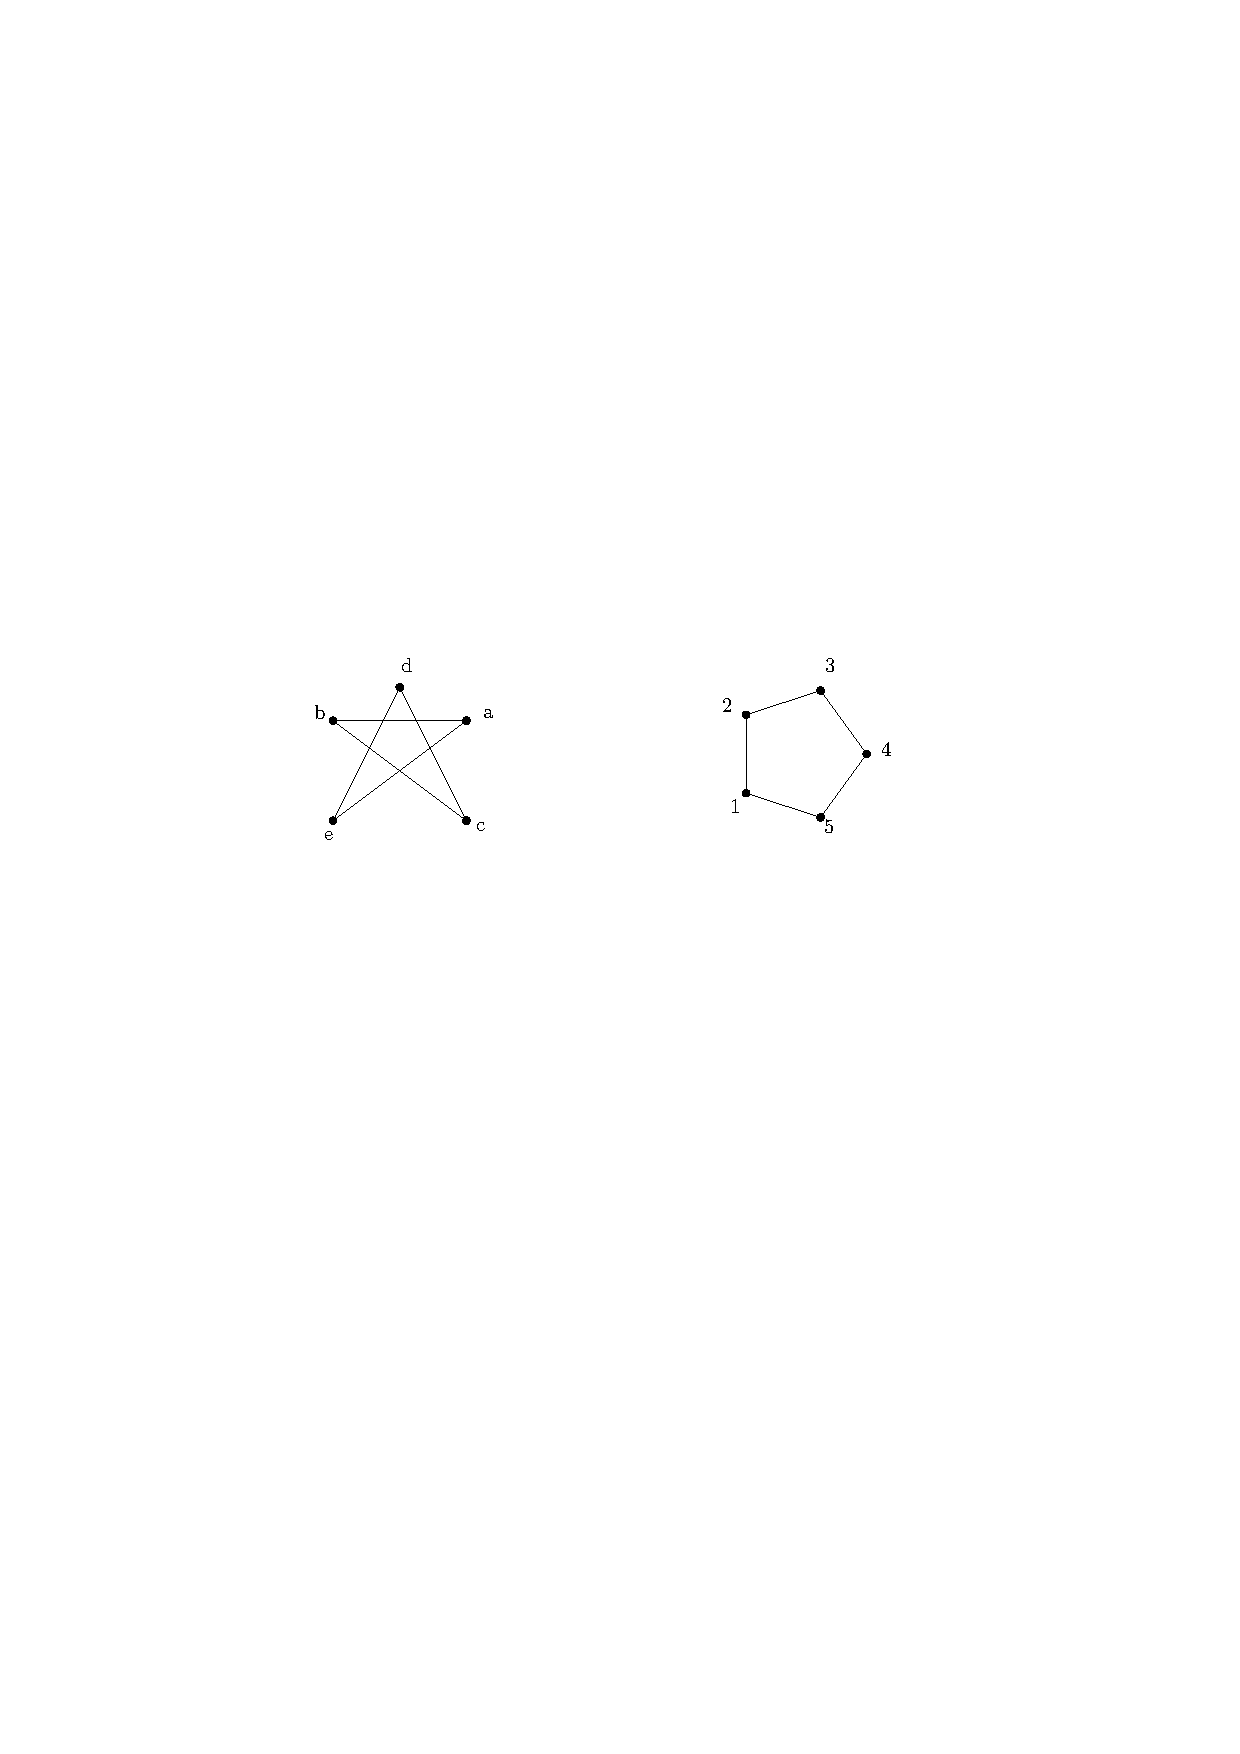
\includegraphics[scale=1]{graphics/graphIsomorphismExample.pdf}
\end{center} 
\caption{This figure depicts the graph isomorphism shown in Table \ref{table:ch1-graph-1} between $V_1$ and $V_2$.}
\label{fig:configuration-3}
\end{figure}

To visualize a graph, $G$, we create a drawing $\Pi$, of $G$.  
The \textit{drawing} of a graph $G=(V,E)$ is an injective mapping $\Pi : V \mapsto \bbR^{2}$ which maps vertices to distinct points in the plane and for each edge $\curlybraces{u,v} \in E$, a continuous, injective mapping $c_{u,v}:[0,1]\mapsto \bbR^2$ such that $c_{u,v}(0) = \Pi(u)$, $c_{u,v}(1) = \Pi(v)$, and the curve $c_{u,v}$ does not pass through any other vertex in $V$.
In this thesis, we will work with straight line drawings and orthogonal drawings.
Straight line drawings have mappings $c_{u,v}$ that are straight line segments.
Orthogonal drawings have mappings $c_{u,v}$ which are a sequence of alternating horizontal line segments and vertical line segments.
For orthogonal drawings, the endpoint of one line segment is the starting point of the next line segment, i.e. every $c_{u,v}$ is piecewise continuous.
The endpoints of the line segments of $c_{u,v}$ that are not $\Pi(u)$ or $\Pi(v)$ are called $\textit{bends}$.

\begin{figure}[!htbp]
\begin{center}
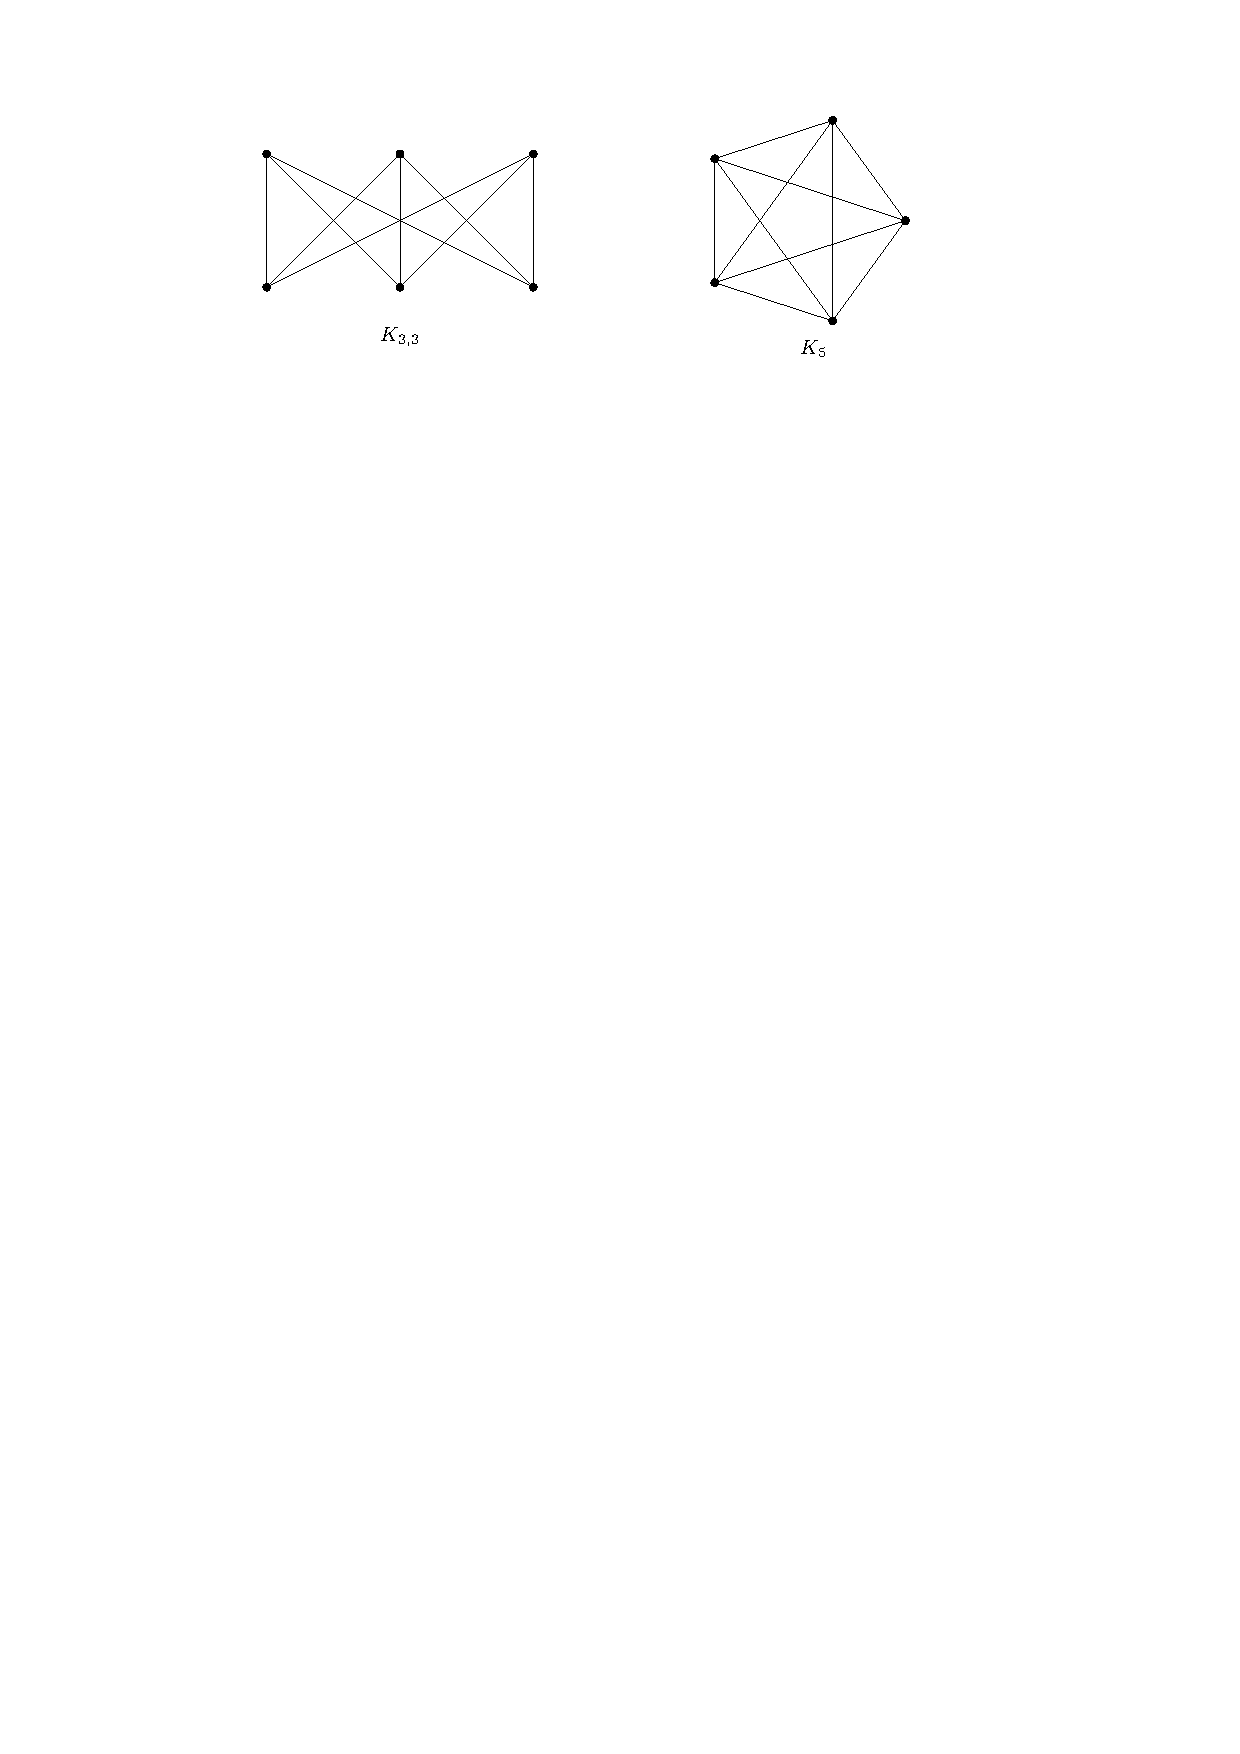
\includegraphics{graphics/kuratowskiExamples.pdf}
\caption{The $K_5$ and $K_{3,3}$ drawn in the plane.}\label{fig:kuratowskiExamples.pdf}
\end{center} 
\end{figure} 
Kuratowski's theorem characterizes finite planar graphs.
A finite graph is planar if and only if it does not contain a subgraph that is a subdivision of $K_5$ or $K_{3,3}$ \cite{kuratowski1930probleme}. 
Figure \ref{fig:kuratowskiExamples.pdf} shows a drawing of $K_5$ and $K_{3,3}$.
Two edges in a drawing \textit{cross} if they have a common interior point.  
The \textit{crossing number} of a graph is the smallest number of edge crossings for a graph over all drawings.
A drawing is said to be \textit{planar} if no two distinct edges cross \cite{BET+99}.
A planar drawing is also called an \textit{embedding}.
Two embeddings of a graph $G$ are \textit{equivalent} if for every vertex the counter-clockwise order of neighbors are the same.  
A combinatorial \textit{embedding} is a planar drawing with a corresponding counter-clockwise order of the neighbors of each vertex. 
\begin{figure}[!htbp]
\begin{center}
    \includegraphics{graphics/combinatorialEmbedding.pdf}
    \caption{Here is a wheel graph, $W_5$, in two separate drawings with the same counterclockwise ordering of neighbors for each vertex.}\label{fig:combinatorialEmbedding.pdf}
\end{center}
\end{figure}
An orientation preserving rigid transformation (i.e., rotation and translation) map an embedding to an equivalent embedding.  
Reflections reverse the counter-clockwise order around each vertex.

Figure \ref{fig:combinatorialEmbedding.pdf} depicts two different drawings of the wheel graph $W_5$.  
The drawings have the counterclockwise order of neighbors for each vertex shown in Table \ref{table:combinatorialEmbedding}.  
Referencing Table \ref{table:combinatorialEmbedding} and Figure \ref{fig:combinatorialEmbedding.pdf}, we realize that the two drawings of $W_5$ are equivalent.  

\begin{table}[!htbp]
\begin{center}
\begin{tabular}{|C|C|C|}\hline
\text{Vertex}&\text{Left \& Middle Drawing}&\text{Right Drawing}\\\hline
1&(2,5,4)& (4,5,2) 
\\\hline
2&(3,5,1) & (1,5,3) 
\\\hline
3&(2,4,5)& (5,4,2) 
\\\hline
4& (1,5,3)  & (3,5,1) 
\\\hline
5&(2,3,4,1)& (4,3,2,1) 
\\\hline
\end{tabular} 
\caption{A table showing the counter-clockwise circular ordering of neighbors for the left and right drawing in Figure \ref{fig:combinatorialEmbedding.pdf}.  Note that the permutation cycles are equivalent for the right and left drawings.}\label{table:combinatorialEmbedding}
\end{center} 
\end{table}

\subsection{Trees}
A \textit{path} is a sequence of vertices in which every two consecutive vertices are connected by an edge.   
\noindent%
\begin{minipage}{\linewidth}
\begin{center}
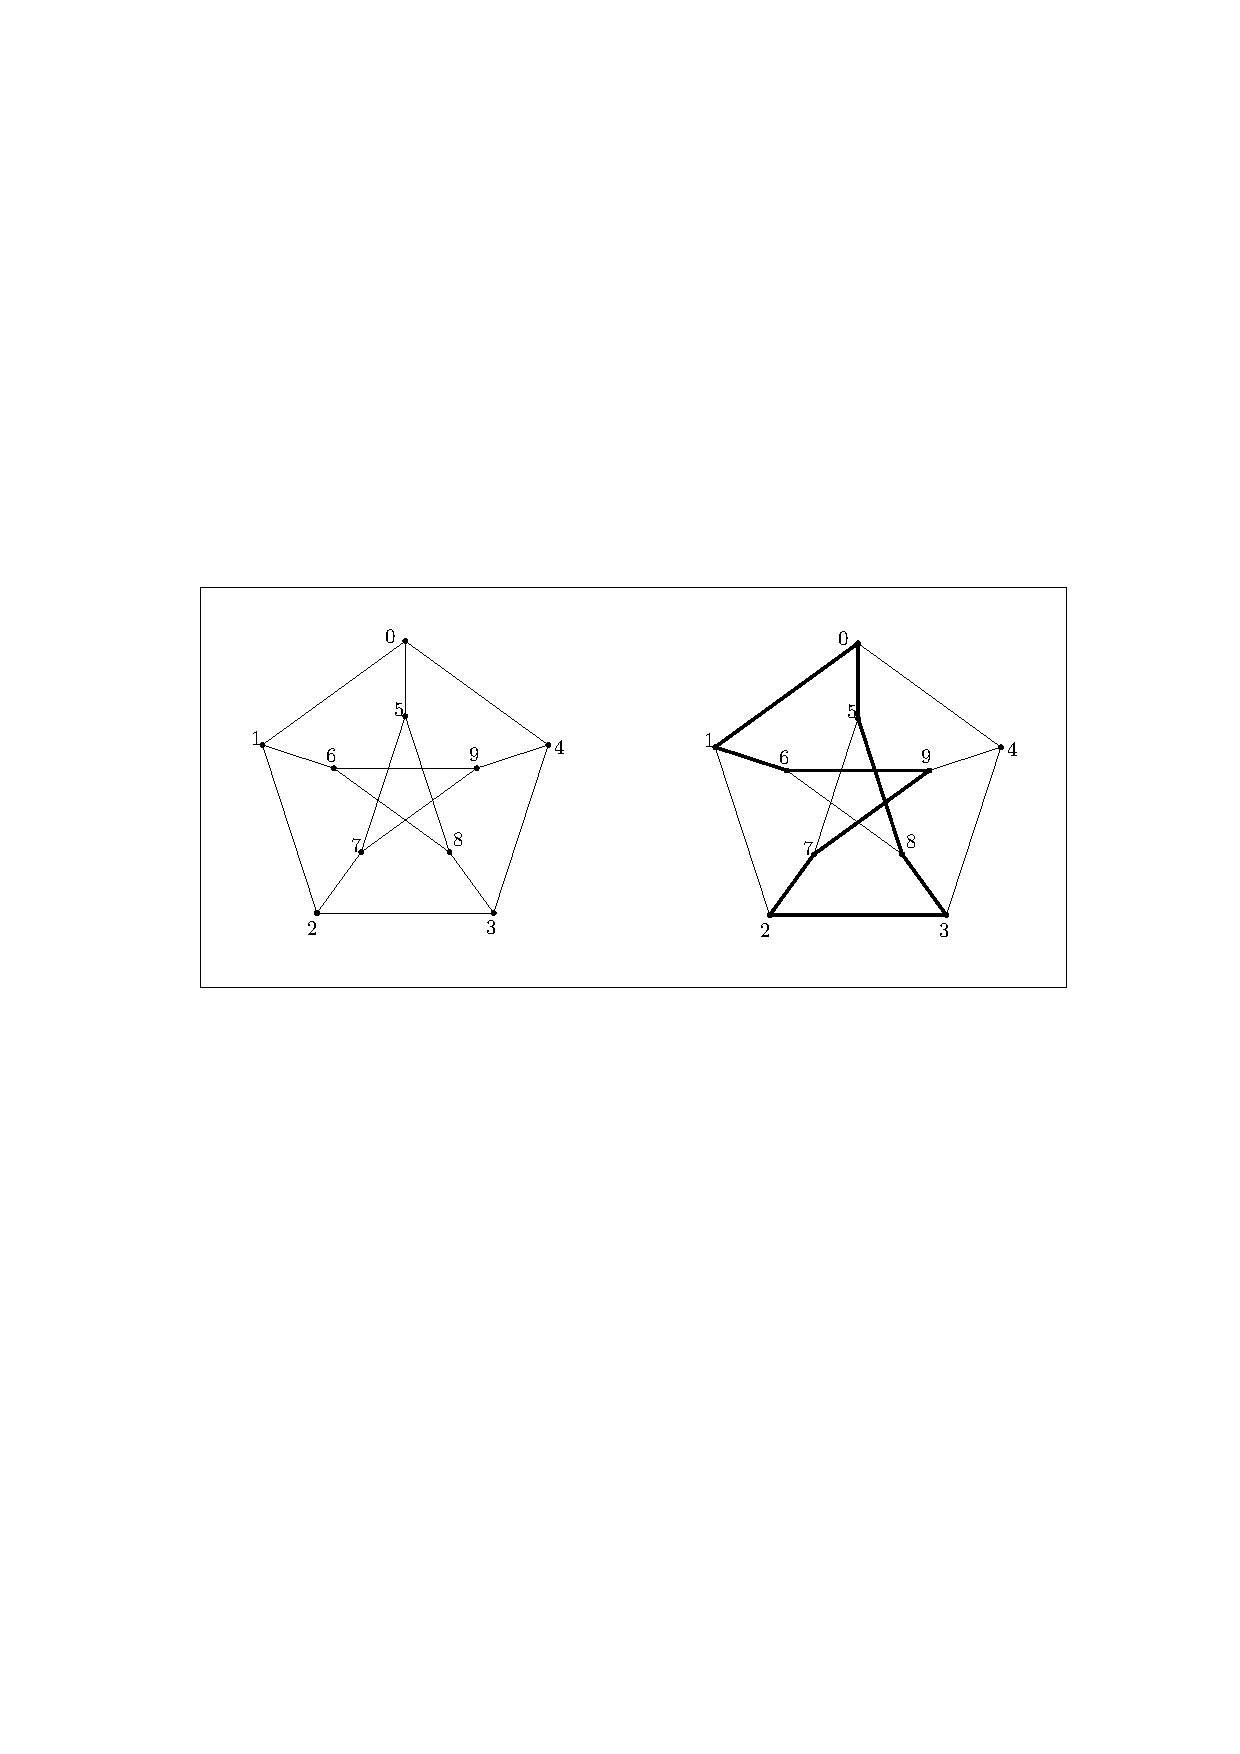
\includegraphics{graphics/PetersonGraphWithPath.pdf}
\captionof{figure}{An embedding of the Peterson graph with a simple cycle of 
(2,7,9,6,1,0,5,8,3).}\label{fig:PetersonGraphWithPath}
\end{center}
\end{minipage}
A \textit{simple cycle} of a graph is a sequence, $(v_1, v_2, \ldots, v_{t-1},v_t)$, of distinct vertices such that every two consecutive vertices are connected by an edge,  and the last vertex, $v_t$, connects to $v_1$ (see Figure \ref{fig:PetersonGraphWithPath}).  
A graph is \textit{connected} if for any two vertices, there exists a path between the two points.
A \textit{tree} is a graph that has no simple cycles and is connected (see Figure \ref{fig:ch1-graph-2}).
Every tree is planar.
A \textit{forest} is a disjoint union of trees.  
\noindent%
\begin{minipage}{\linewidth}
\begin{center}
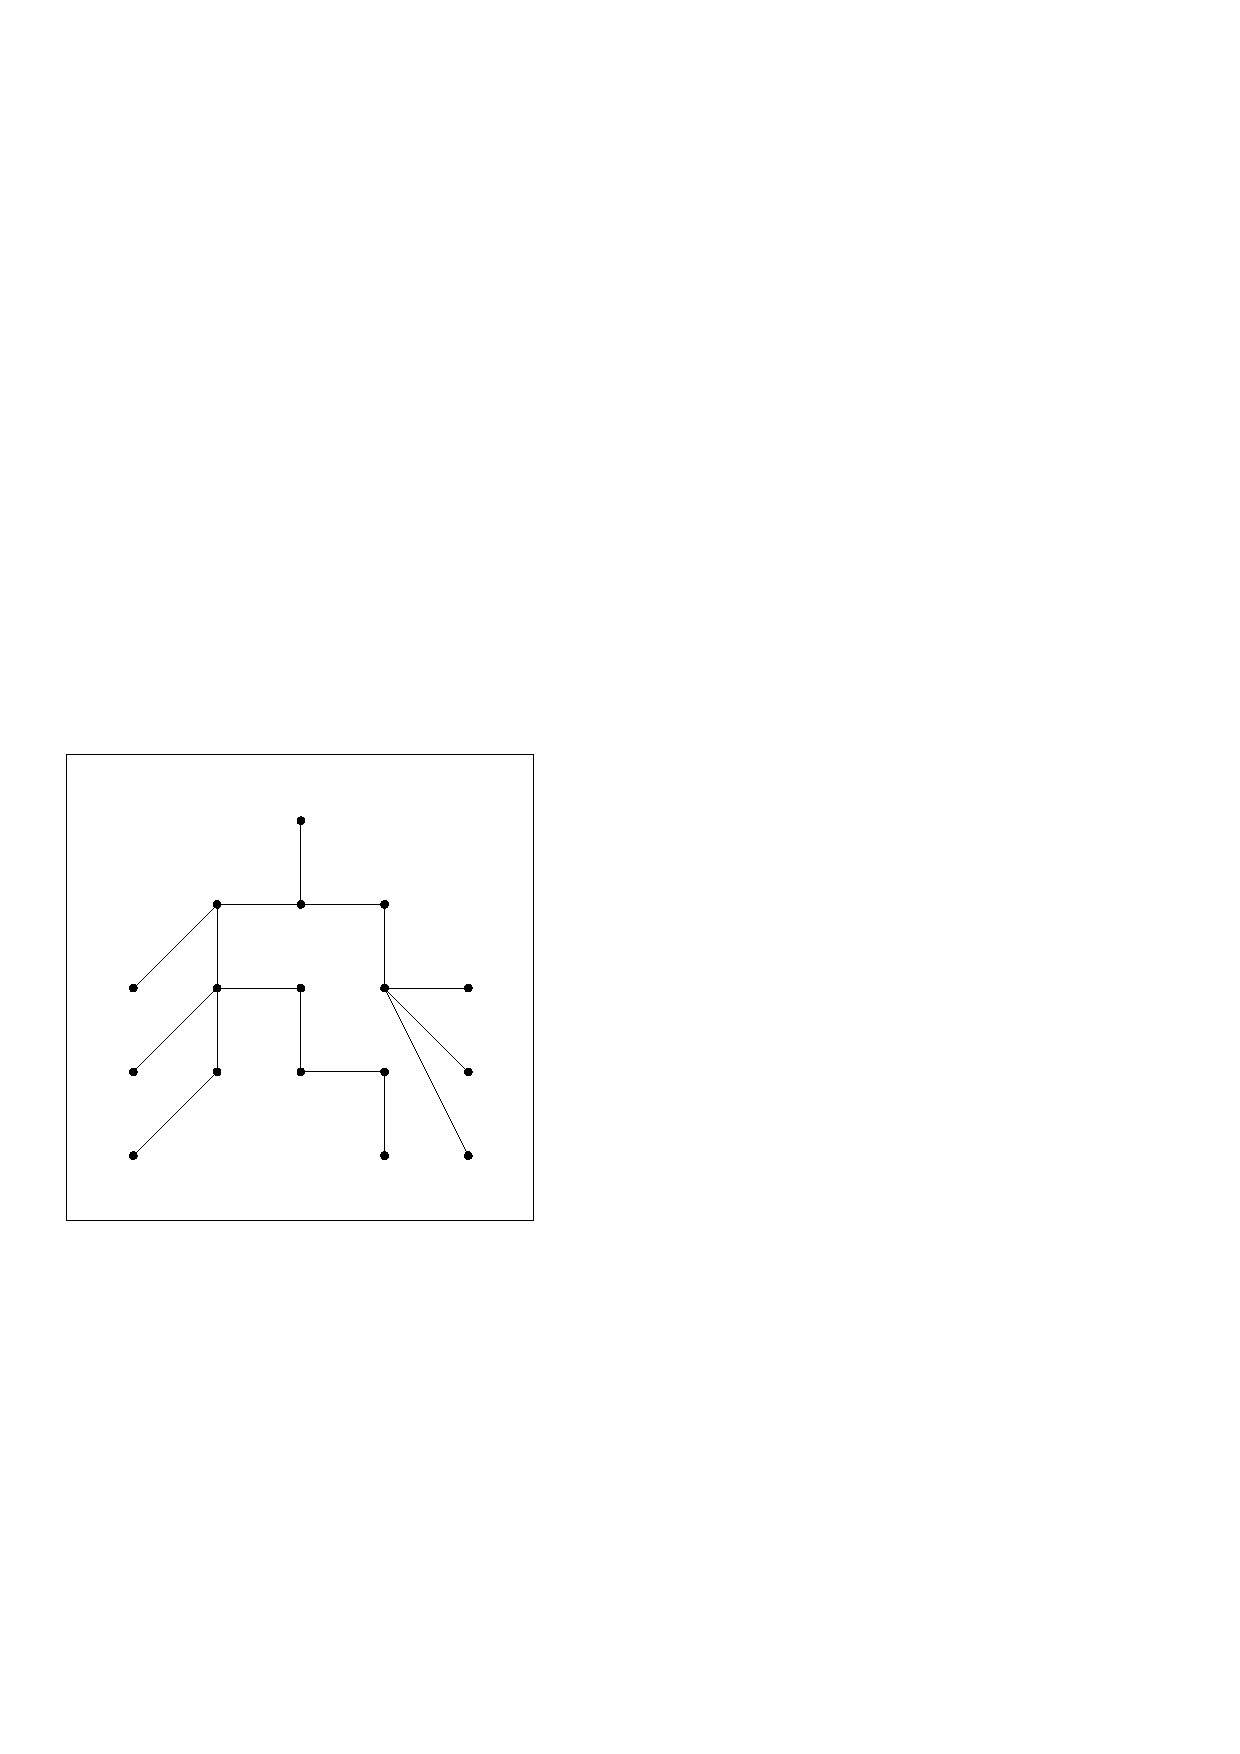
\includegraphics{graphics/RandomTree.pdf}
\captionof{figure}{An example of a tree.}\label{fig:ch1-graph-2}
\end{center}
\end{minipage}

An \textit{ordered tree} is a tree $T$ together with a cyclic order of the neighbors for each vertex (see Figure \ref{fig:ch1-graph-6}).
\noindent%
\begin{minipage}{\linewidth}
\begin{center}
    \includegraphics{graphics/OrderedTreesExample.pdf}
    \captionof{figure}{A tree with two embeddings with different cyclic orderings around 
vertices.}\label{fig:ch1-graph-6}
\end{center}
\end{minipage}

\textit{Embeddings} of ordered trees are combinatorially equivalent if for each node the counter-clockwise ordering of adjacent nodes are the same. 

\section{Linkages}

\begin{minipage}{\linewidth}
\begin{center}
\includegraphics{graphics/HumanTurkeyLinkage.pdf}
\captionof{figure}{Here are skeleton drawings of a human and a turkey.  When animating skeletons, one tends to make sure that the lengths of the skeleton segments are kept the same length throughout the animation.  Otherwise, the animation may depart from what is ideally understood of skeletal motions.}\label{fig:turkey}
\end{center}
\end{minipage}

When graph drawings model physical objects, other qualities about the graph can be contextualized in a geometric sense.  
Distance, angular relationships and other geometric qualities may be relevant.
In any drawing, edges have length, angles formed by adjacent edges, and so on.  
In this thesis we are interested in the inverse problem where we would like to embed a graph with specific geometric properties, for example, an embedding with specified edge lengths. 
This motivates the following definition.
A \textit{length assignment} of a graph $G=(V,E)$ is a function $\ell:E \mapsto \bbr^+$. 
If $\ell(e)$ is the length of an edge $e$, $\ell(e)$ must be strictly positive in a drawing, otherwise it may result in two distinct vertices with the same coordinates.
Similar to combinatorial embeddings which is an equivalence class of embeddings of the same counter-clockwise order of vertices, we can also define an equivalence class of drawings with the same length assignment.
A \textit{linkage} is a graph $G = (V,E)$ with a length assignment $\ell:E \mapsto \bbr^+$ (e.g. see Figure \ref{fig:turkey}).
\section{Polygonal Linkages}\label{sec:hinge}
A generalization of linkages is a polygonal linkage where edges of given lengths are replaced with rigid polygons.
Formally, a \textit{polygonal linkage} is an ordered pair $\left(\PP,\HH \right)$ where $\PP$ is a finite set of polygons and $\HH$ is a finite set of hinges; a \textit{hinge} $h\in \HH$ corresponds to two or more points on the boundary of distinct polygons in $\PP$.  
A \emph{realization of a polygonal linkage} is an interior-disjoint placement of congruent copies of the polygons in $\PP$ such that the copies of a hinge are mapped to the same point (e.g., Figure \ref{fig:linkage-1}).  
A \textit{hinge graph} is a bipartite graph where one partite set is the set of polygons $\PP$ and the other partite set is the set of hinges $\HH$.  
There is exists an edge between a polygon and a hinge if the hinge lies on the boundary of the polygon.
\begin{figure}[!htbp]
\begin{center}
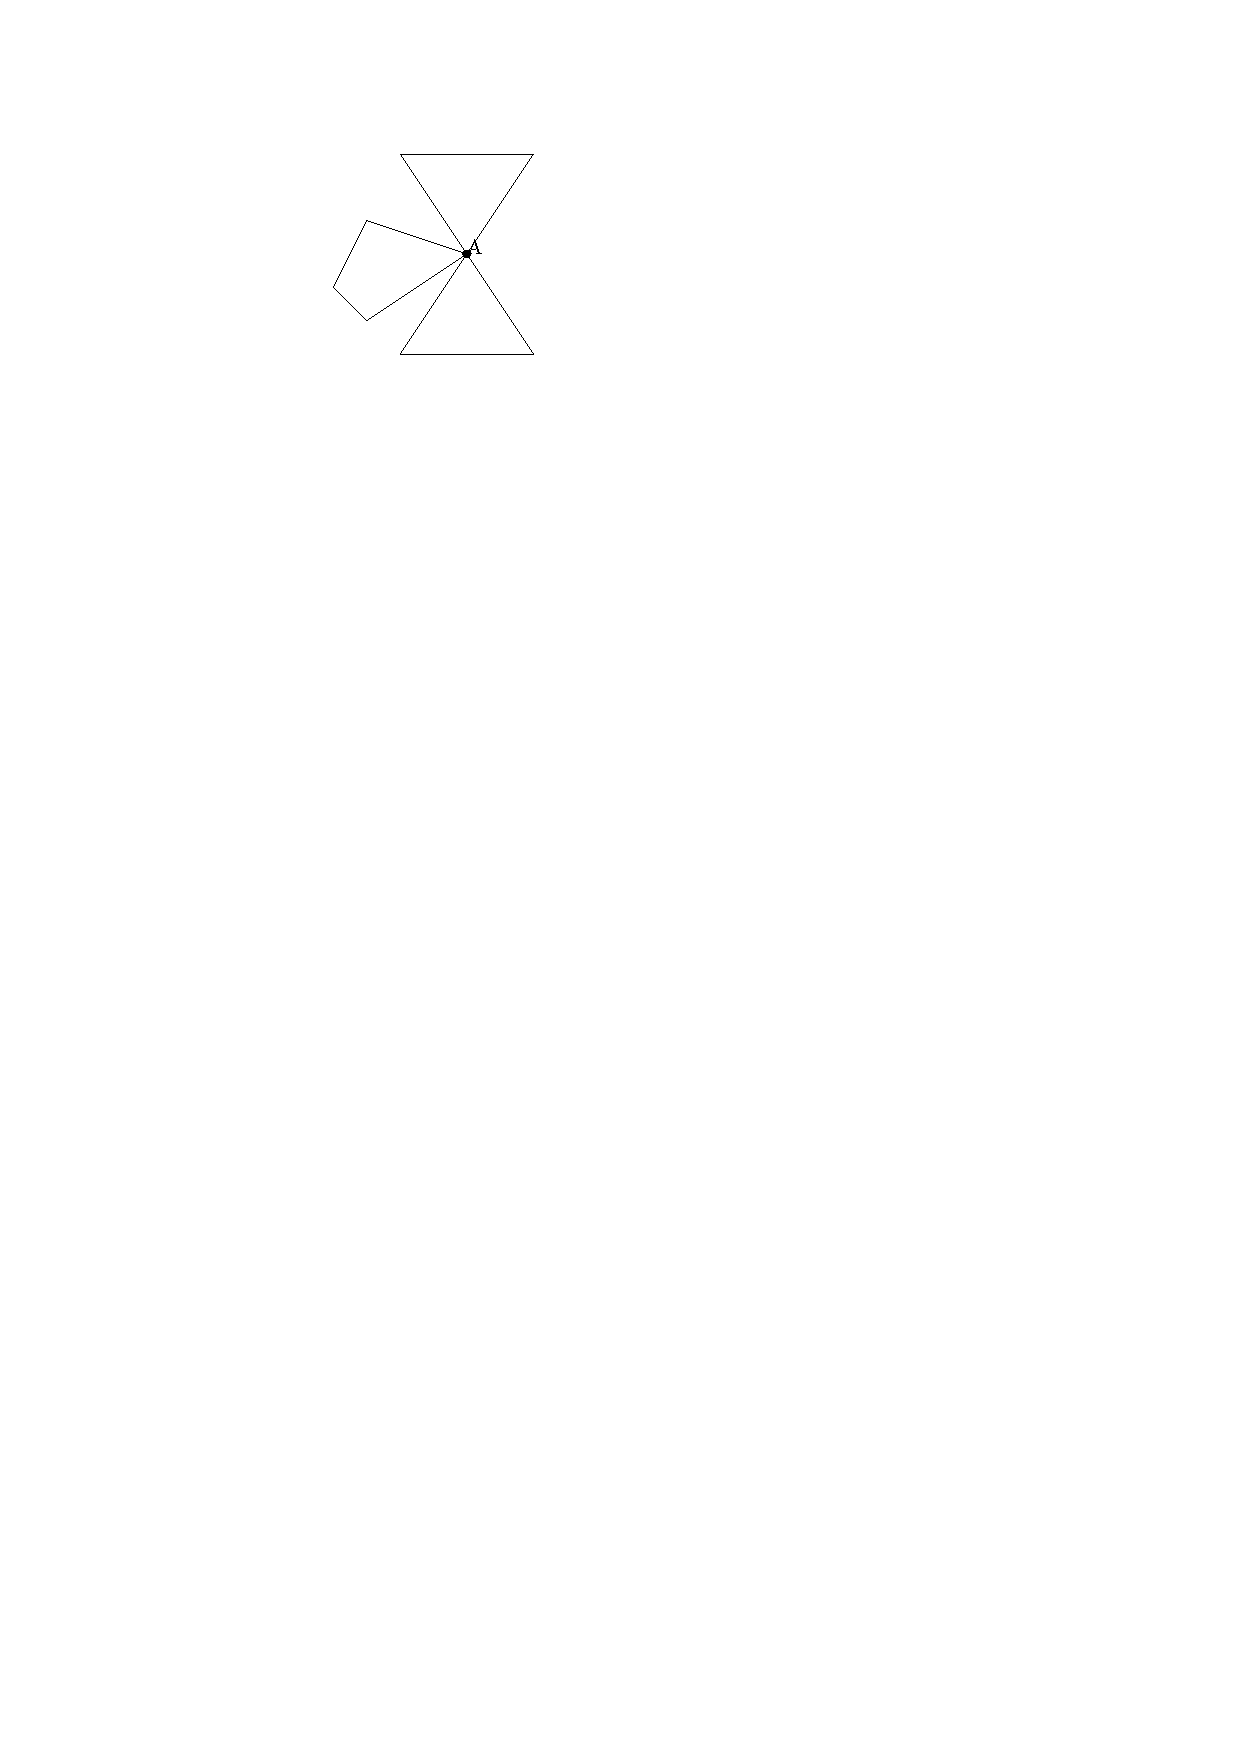
\includegraphics[scale=1]{graphics/hingeOnThreeDistinctPolygons.pdf}
\end{center} 
\caption{(a) A polygonal linkage with a non-convex polygon and two hinge points corresponding to 
three polygons.  Note that hinge points correspond to two distinct polygons.(b) Illustrating that 
two hinge points can correspond to the same boundary point of a polygon.}
\label{fig:linkage-1}
\end{figure}
A \textit{realization of a polygonal linkage with fixed orientation} is a realization in which each polygon is translated and rotated copy of a polygon in $\PP$; at each hinge the incident polygons are in a given counter-clockwise order (refer to Figure \ref{fig:orderedLinkages}).

\begin{minipage}{\linewidth}
\begin{center}
\includegraphics{graphics/orderedLinkages.pdf}
\captionof{figure}{Two realizations of the same polygonal linkage with that differ in the counter-clockwise order of polygons around vertex $a$. }\label{fig:orderedLinkages}
\end{center}
\end{minipage}

Note that oriented polygonal linkage realizations do not allow for reflection transformations of polygons in $\PP$.

These two realization types allow one to pose two different problems, the realizability problem for polygonal linkages and the realizability problem for polygonal linkages with fixed orientation:
\begin{prob}[Realizibility Problem for Polygonal Linkages]\label{problem:UnorderedPolygonal}

Given a polygonal linkage, does it have a realization?
\end{prob}
\begin{prob}[ Realizibility Problem for Polygonal Linkages with Counter-Clockwise Orientation]\label{problem:OrderedPolygonal}
Given a polygonal linkage with fixed orientation, does it have a realization?
\end{prob}
Not every polygonal linkage has a realization.
\begin{figure}[!htbp]
\begin{center}
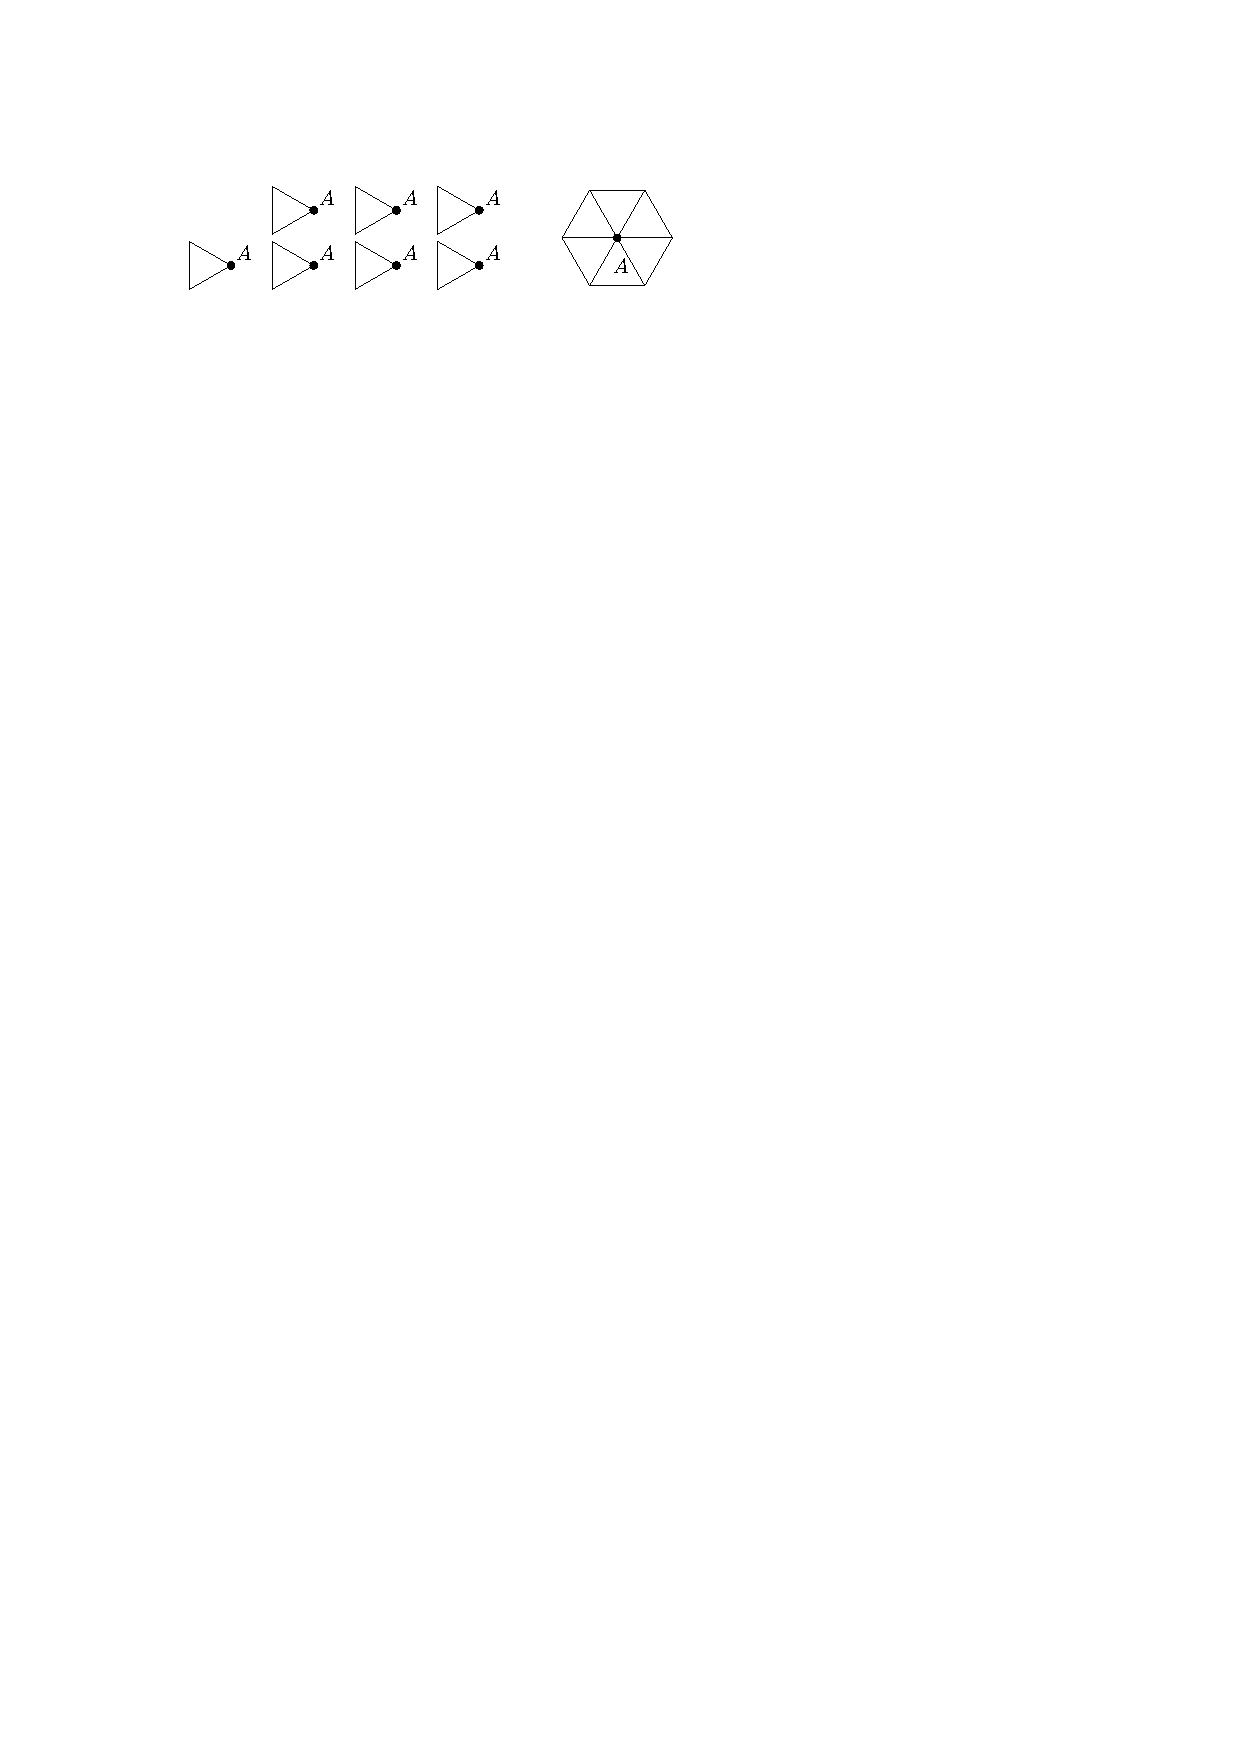
\includegraphics[scale=1]{graphics/Problem1.pdf}
\end{center} 
\caption{Here we have 7 congruent copies of an equilateral triangle with a hinge point of $A$.  The polygonal linkage is not realizable.  The best we can realize is at most 6 congruent copies of an equilateral triangle with the hinge point of $A$ in the plane.}
\label{fig:problem1}
\end{figure}
Consider the 7 congruent copies of an equilateral triangle with a common hinge point in Figure \ref{fig:problem1}.
To show it does not have a realization, suppose it is realizable.  
Each angle of every triangle is $\frac{\pi}{3}$ radians.  
The sum of 7 angles formed by the triangles is $\frac{7\pi}{3}>2\pi$.  
The total radian measure around $A$ is $2 \pi$.
The contradiction is that the sum of 7 angles formed by the triangles in an interior disjoint placement is $\frac{7\pi}{3}$.
The polygonal linkage of Figure \ref{fig:problem1} would overlap itself and does not have a realization.

There are polygonal linkages that admit realizations but every realization requires rotation.
Figure \ref{fig:collidingHingedPolygons} show the congruent copies of the polygons $A$, $B$, $C$, and $D$ in two different configurations, the far right is a realization, the middle fails to be a realization because of the interiors of $B$ and $D$ intersecting and the left showing the polygons in $\PP$.  
In fact, this polygonal linkage cannot admit a realization with fixed orientation.
Indeed this polygonal linkage cannot satisfy Problem \ref{problem:OrderedPolygonal}, suppose there is a realization with fixed orientation.  
Without loss of generality, fix the placement of $C$.
$A$, $B$, and $D$ have unique placement around triangle $C$.  
In this placement $C$ and $D$ overlap.
\begin{figure}[!htbp]\begin{center}
\includegraphics[scale=1]{graphics/collidingHingedPolygons.pdf}
\end{center} 
\caption{This example shows yet another example where two realizations of the same polygonal linkage. 
 One realization where there is an intersection and another where there isn't an intersection.}\label{fig:collidingHingedPolygons}
\end{figure}
Figure \ref{fig:collidingHingedPolygons}, satisfies Problem \ref{problem:UnorderedPolygonal} but not Problem \ref{problem:OrderedPolygonal}.
 The far right is a realization but with polygon $B$ reflected. 

Figure \ref{fig:collidingHingedPolygons} does not quite get at the heart of the challenge with Problem \ref{problem:UnorderedPolygonal} because the counter-clockwise order of the polygons around hinges is not considered.

\begin{minipage}{\linewidth}
\begin{center}
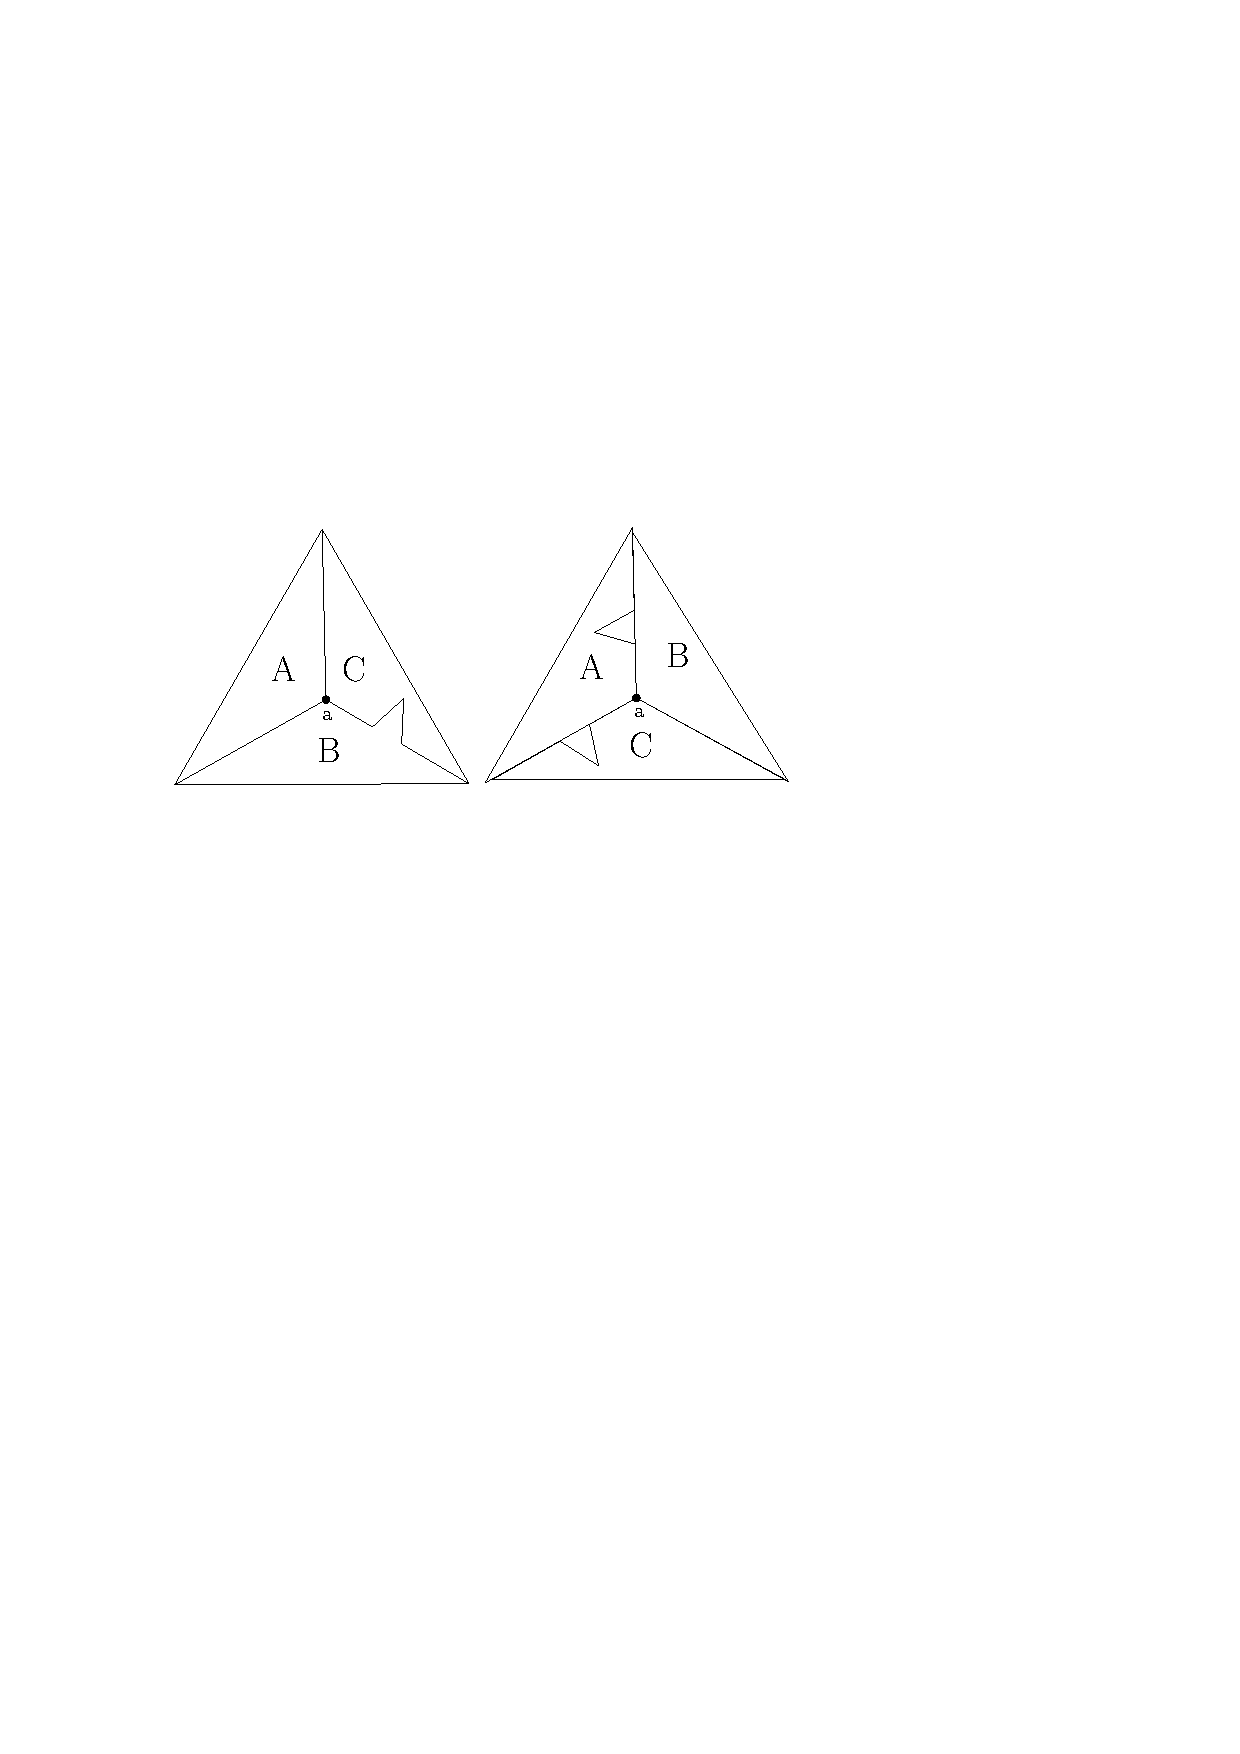
\includegraphics[width=.33\columnwidth]{graphics/orderedFaces.pdf}
\end{center}
\captionof{figure}{Here we have two realizations of a polygonal linkage with two different counter-clockwise order (C,B,A) and (B,C,A) respectively.  
Note that the placement with ordering (B,C,A) has an overlap.}\label{fig:orderedFaces.pdf}
\end{minipage}

Figure \ref{fig:orderedFaces.pdf} shows three polygons with a common hinge.
In the counter-clockwise order $(A,B,C)$, the polygonal linkage admits a realization whereas in the counter-clockwise order $(A,C,B)$, it does not admit a realization.
The examples above show that answers to Problem \ref{problem:UnorderedPolygonal} and \ref{problem:OrderedPolygonal} could be yes or no; the answer could be negative for various reasons.
Sections 2 and 3 of this thesis address the computational complexity of solving Problems \ref{problem:UnorderedPolygonal} and \ref{problem:OrderedPolygonal}.
We show that both problems are intractable.




\subsection{Geometric Dissections}
Hilbert's third problem asks: given any two polyhedra of equal volume, is it always possible to cut the first into finitely many polyhedral pieces which can be reassembled to yield the second \cite{aigner2010hilbert}?  
In three dimensions the answer is no however for two dimensions it is true \cite{10.23073621846}.

The Wallace-Bolyai-Gerwien Theorem simply states that two polygons are congruent by dissection if and only if they have the same area.  
A \textit{dissection} being a collection of smaller polygons whose interior disjoint union forms a polygon.
Hinged dissections of a polygon $P$ is a polygonal linkage that admits a realization that forms $P$.  
Demaine et. al. \cite{abbott2012hinged} showed that any two polygons of the same area have a common hinged dissection where polygonal pieces must hinge together at vertices to form a connected realization and that there exists a continuous motion between the two realizations (refer to section 1.5.3).
The was an outstanding problem for many years until 2007.

The Haberdasher Puzzle was proposed in 1902 by Henry Dudeney: can a square and an equilateral triangle of the same area have a common dissection into four pieces? 

\begin{minipage}{\linewidth}
\begin{center}
\includegraphics{graphics/HaberdasherProblem.pdf}
\end{center}
\captionof{figure}{The Haberdasher Puzzle was proposed in 1902 and solved in 1903 by Henry Dudeny.  The dissection is for polygons that forms a square and equilateral triangle.}
\label{fig:polygonallinkage-5}
\end{minipage}

Geometric dissections are closely related to polygonal linkages.  
Figure \ref{fig:polygonallinkage-4} shows two arrangements of the same polygons to form a hexagon and a square. 
The polygons are not hinged and are arranged in differing order.
The polygons are merely tiled together to form the hexagon and square. 

\begin{minipage}{\linewidth}\begin{center}
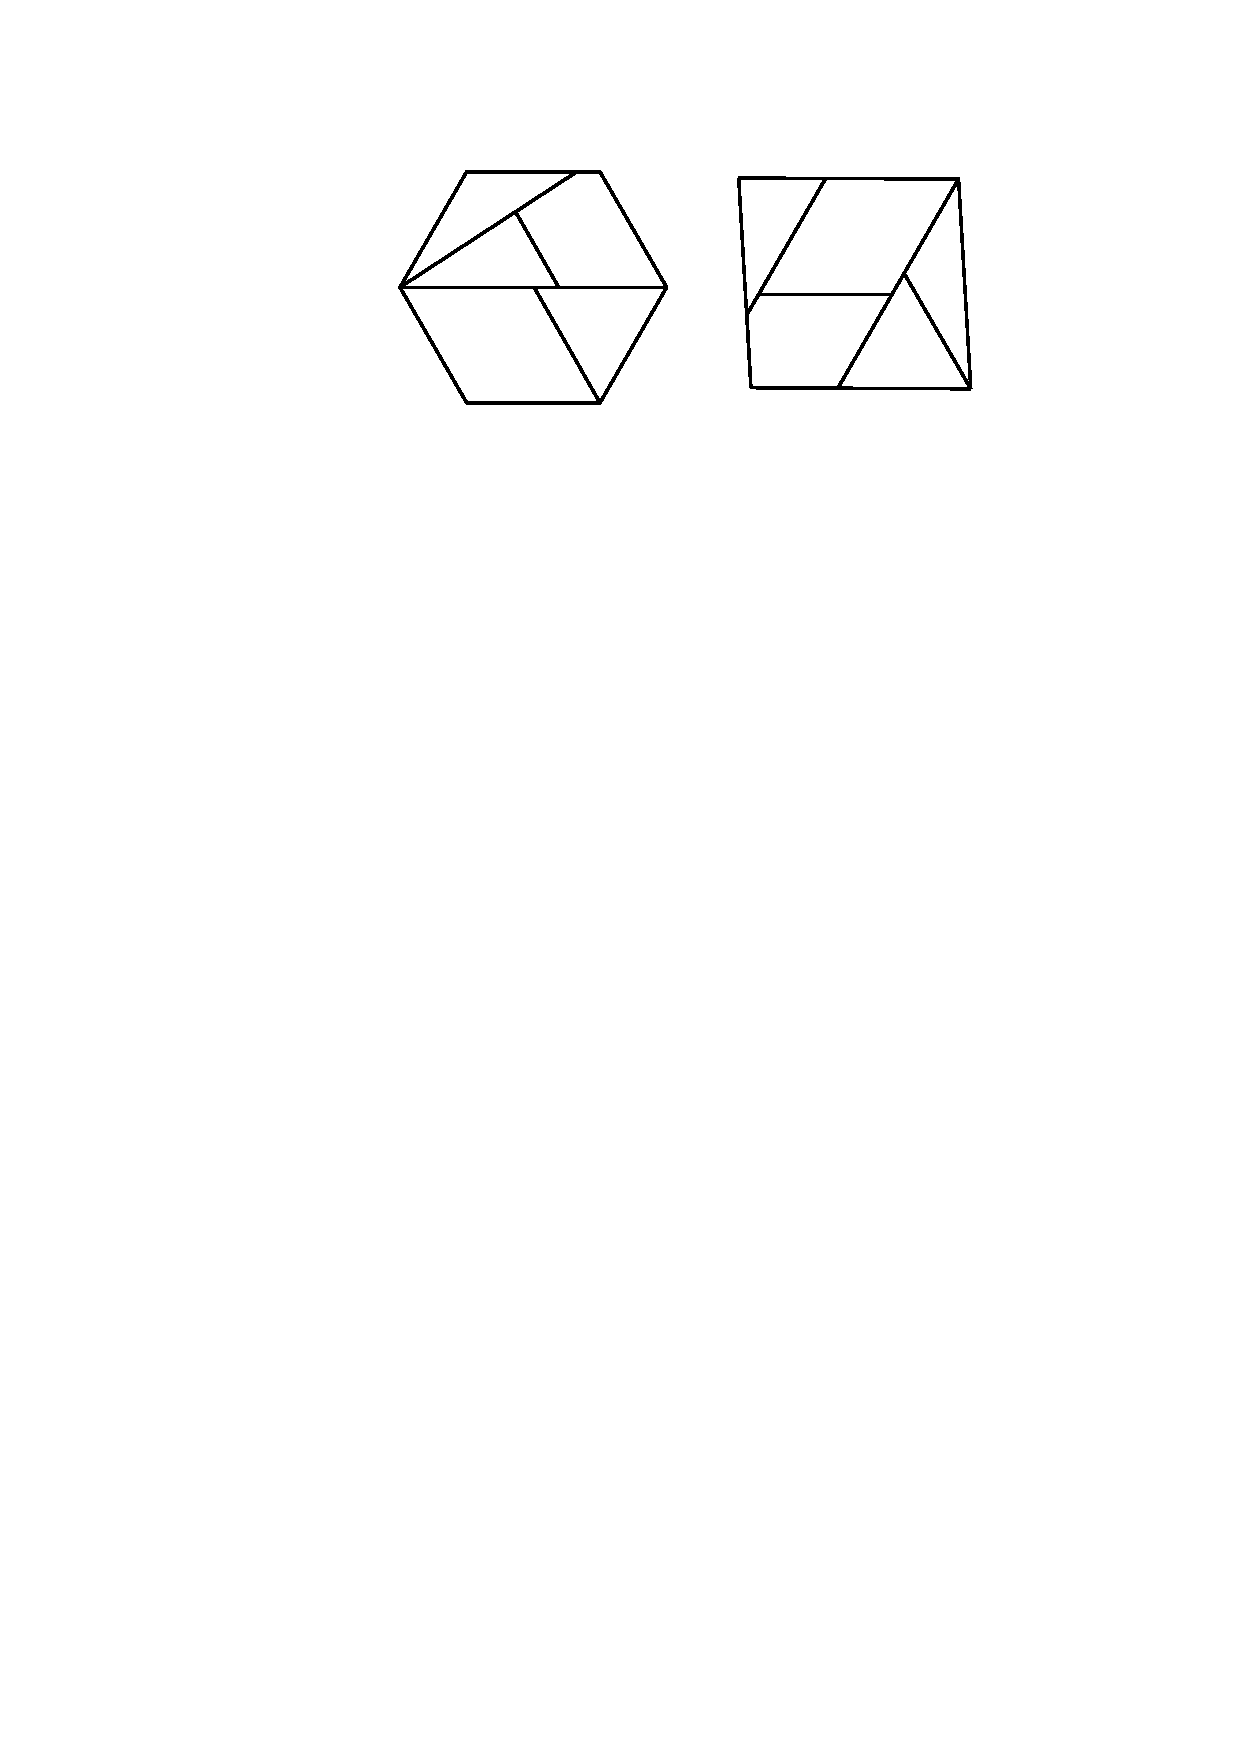
\includegraphics{graphics/GeometricDissectionBusschop.pdf}
\end{center}
\captionof{figure}{Two configurations of polygonal linkage where the polygons touch on boundary segments 
instead of hinges.  These two realizations of the polygonal linkage are invalid to our definitions. 
 }
\label{fig:polygonallinkage-4}
\end{minipage}

Figure \ref{fig:HingedHaberdasher}, shows the Haberdasher problem with hinges.  
This makes the Haberdasher problem as a type of polygonal linkage where the polygons are free to move about their hinge points and take the form of a triangle or square.  

\begin{minipage}{\linewidth}
\begin{center}
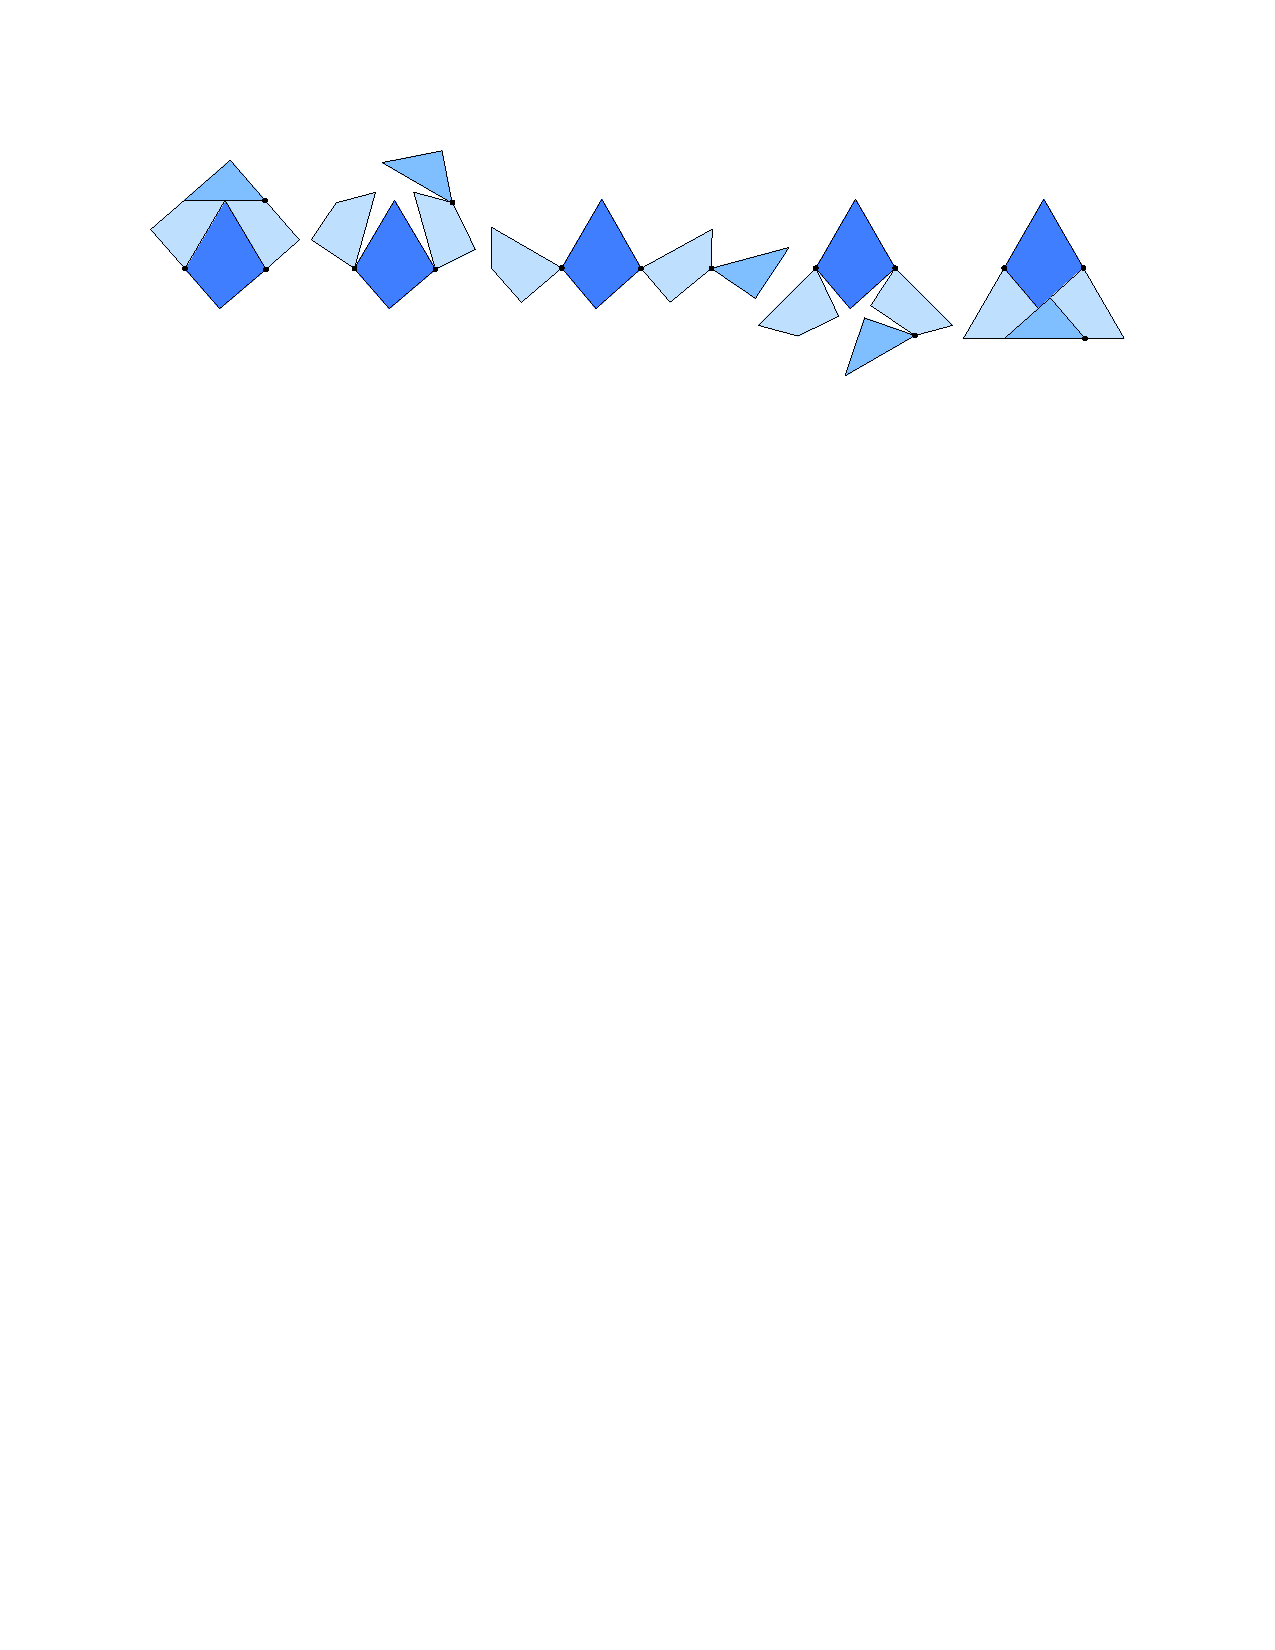
\includegraphics[width=\textwidth]{graphics/HingedHaberdasher.pdf}
\end{center}
\captionof{figure}{This shows the Haberdasher problem in the form of polygonal linkage \cite{abbott2012hinged}.  This is a classic example of two polygons of equal area that have a common hinged dissection.}
\label{fig:HingedHaberdasher}
\end{minipage}


 A \textit{disk arrangement} is a set of interior disjoint disks, $D$.  
 If for any pair of disks in $D$ intersect at a boundary point, they are said to be in contact (kissing).

\begin{minipage}{\linewidth}
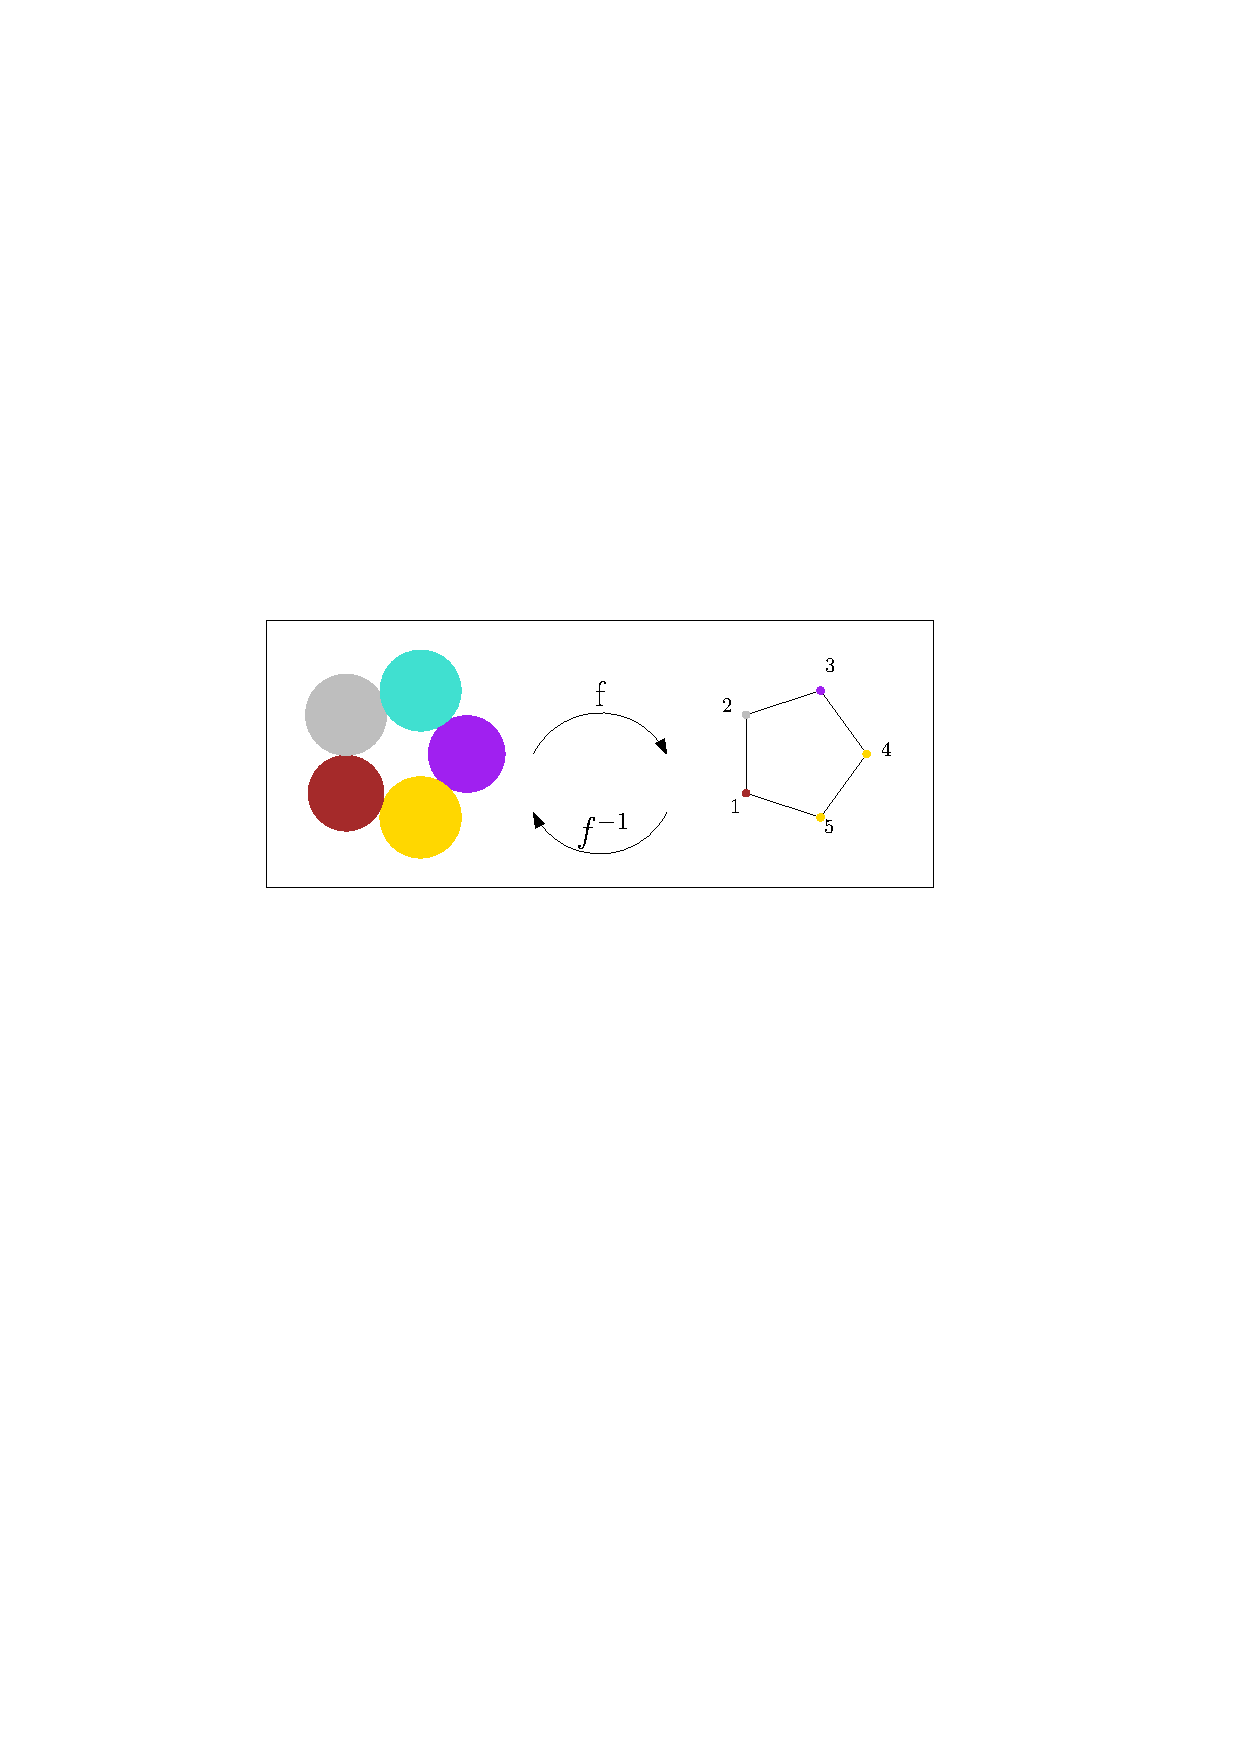
\includegraphics[scale=1]{graphics/diskPackingTheoremExample.pdf}
\captionof{figure}{This example represents a disk arrangement and its contact graph.}
\label{fig:DiskArrangement-1}
\end{minipage}

A \textit{contact graph} $G=(V,E)$ corresponding to a given disk arrangement where there is a bijection $b_V: V \mapsto D$ and a bijection that maps an edge $e_{i,j} \in E$ to an interior disjoint pair of disks $d_i$, $d_j \in D$ (see Figure \ref{fig:DiskArrangement-1}).
Given a disk arrangement, the contact graph can be thought of as a linkage because the distance between two kissing disk equal the sum of radii.  
However if the two disks don't kiss, the distance between their centers is strictly greater than the sum of their radii.
Given a disk arrangement, the contact graph can be thought of as a linkage because the distance between two kissing disk equal the sum of radii.  
However if the two disks don't kiss, the distance between their centers is strictly greater than the sum of their radii.

Koebe's theorem states that for every planar graph $G$, there exists a planar disk arrangement whose contact graph is $G$ \cite{koebe1936kontaktprobleme}.
This motivates the question of whether a planar graph $G$ is a contact graph of a disk arrangement with given radii.
The radii can be given by a weight function.
Let $\omega: V \mapsto \bbR^+$ be the \textit{weight function}.  
The mapping $\omega$ assigns a weight to each vertex in $V$.  
Let $\Pi:V \mapsto \bbr^2$ be that planar mapping of vertices.

For planar graphs with positive weighted vertices, we pose two realizability problems:
\begin{prob}[Unordered Realizibility Problem for a Contact Graph]\label{problem:UnorderedContactGraph}
Given a planar graph with positive weighted vertices, is it a contact graph of some disk arrangement where the radii equal the vertex weights?
\end{prob}
\begin{prob}[Ordered Realizibility Problem for a Contact Graph]\label{problem:OrderedContactGraph}
Given a planar graph with positive weighted vertices and a combinatorial embedding, is it a contact graph of some disk arrangement where the radii equal the vertex weights and the counter-clockwise order of neighbors of each disk is specified by the combinatorial embedding?
\end{prob}

An instance of Problem \ref{problem:UnorderedContactGraph} is shown in Figure \ref{fig:DiskArrangement-1} where the cycle graph $C_5$ is the contact graph of unit disks.
It is not difficult to see that there exists a planar graph with positive weights with no realizable disk arrangement.
Consider the a star graph with 6 leafs, each vertex with unit weight.
In any realization, the angle between two consecutive edges must be greater than $\frac{\pi}{3}$. 
The sum of 6 angles is $2 \pi$ however, the sum of 6 consecutive angles is greater than $2\pi$.
The contradiction shows that no realization is possible.  
Note that with the wheel graph $W_7$ is realizable as a contact graph of unit disks.

Every path with arbitrary positive radii is realizable as a contact graph, place the vertices on a line.
We show that not all binary trees are realizable, even with unit disks.  % of unit radii.
Consider the balanced binary trees of depth $i$ $\left\lbrace T_i \right\rbrace_{i=1}^\infty$ with unit weights on the vertices (see Figure \ref{fig:circlePacking-1}).
These trees are not realizable for sufficiently large $i$.
\begin{figure}[!htbp]
\begin{center}
  \begin{subfigure}[b]{0.21\textwidth}
	  \includegraphics[width=\textwidth]{graphics/BinaryTree1.pdf}
	  \caption{Binary tree $T_2$.}
	  \label{fig:circlePacking1-1}
  \end{subfigure}
  \begin{subfigure}[b]{0.21\textwidth}
	  \includegraphics[width=\textwidth]{graphics/BinaryTree2.pdf}
	  \caption{Binary tree $T_3$.}
	  \label{fig:circlePacking1-2}
  \end{subfigure}
  \begin{subfigure}[b]{0.21\textwidth}
	  \includegraphics[width=\textwidth]{graphics/BinaryTree3.pdf}
	  \caption{Binary tree $T_4$.}
	  \label{fig:circlePacking1-3}
  \end{subfigure}
  \begin{subfigure}[b]{0.21\textwidth}
	  \includegraphics[width=\textwidth]{graphics/BinaryTree4.pdf}
	  \caption{Binary tree $T_5$.}
	  \label{fig:circlePacking1-4}
  \end{subfigure}
  \caption{ We show the linkages $T_2$ through $T_5$ with distance 2 between adjacent vertices.  }\label{fig:circlePacking-1}
\end{center} 
\end{figure}
Let $i$ be a positive integer and suppose that $T_i$ is a contact graph of unit disks.
The balanced binary tree $T_i$ has $2^i -1$ vertices.
The total area of the disks is $\left( 2^i -1 \right)^2 \cdot \pi$.
We now derive an upper bound for this area.
Suppose the disk corresponding to the root of the tree is centered at the origin.
The centers of the disks at level $j$ are at a distance at most $2\cdot (j-1)$ away from the origin.
The centers of all disks are at distance at most $2 \cdot (i -1)$ away from the origin.
All unit disks are contained in a disk of radius $2i-1$ centered at the origin.
The total area of the disks is at most $(2i-1)^2$.  
A upper bound of the total area of the disk arrangement is the area of the bounding box of the disks.

\begin{figure}[!htpb]
\begin{center}
  \begin{subfigure}[b]{0.24\textwidth}
	  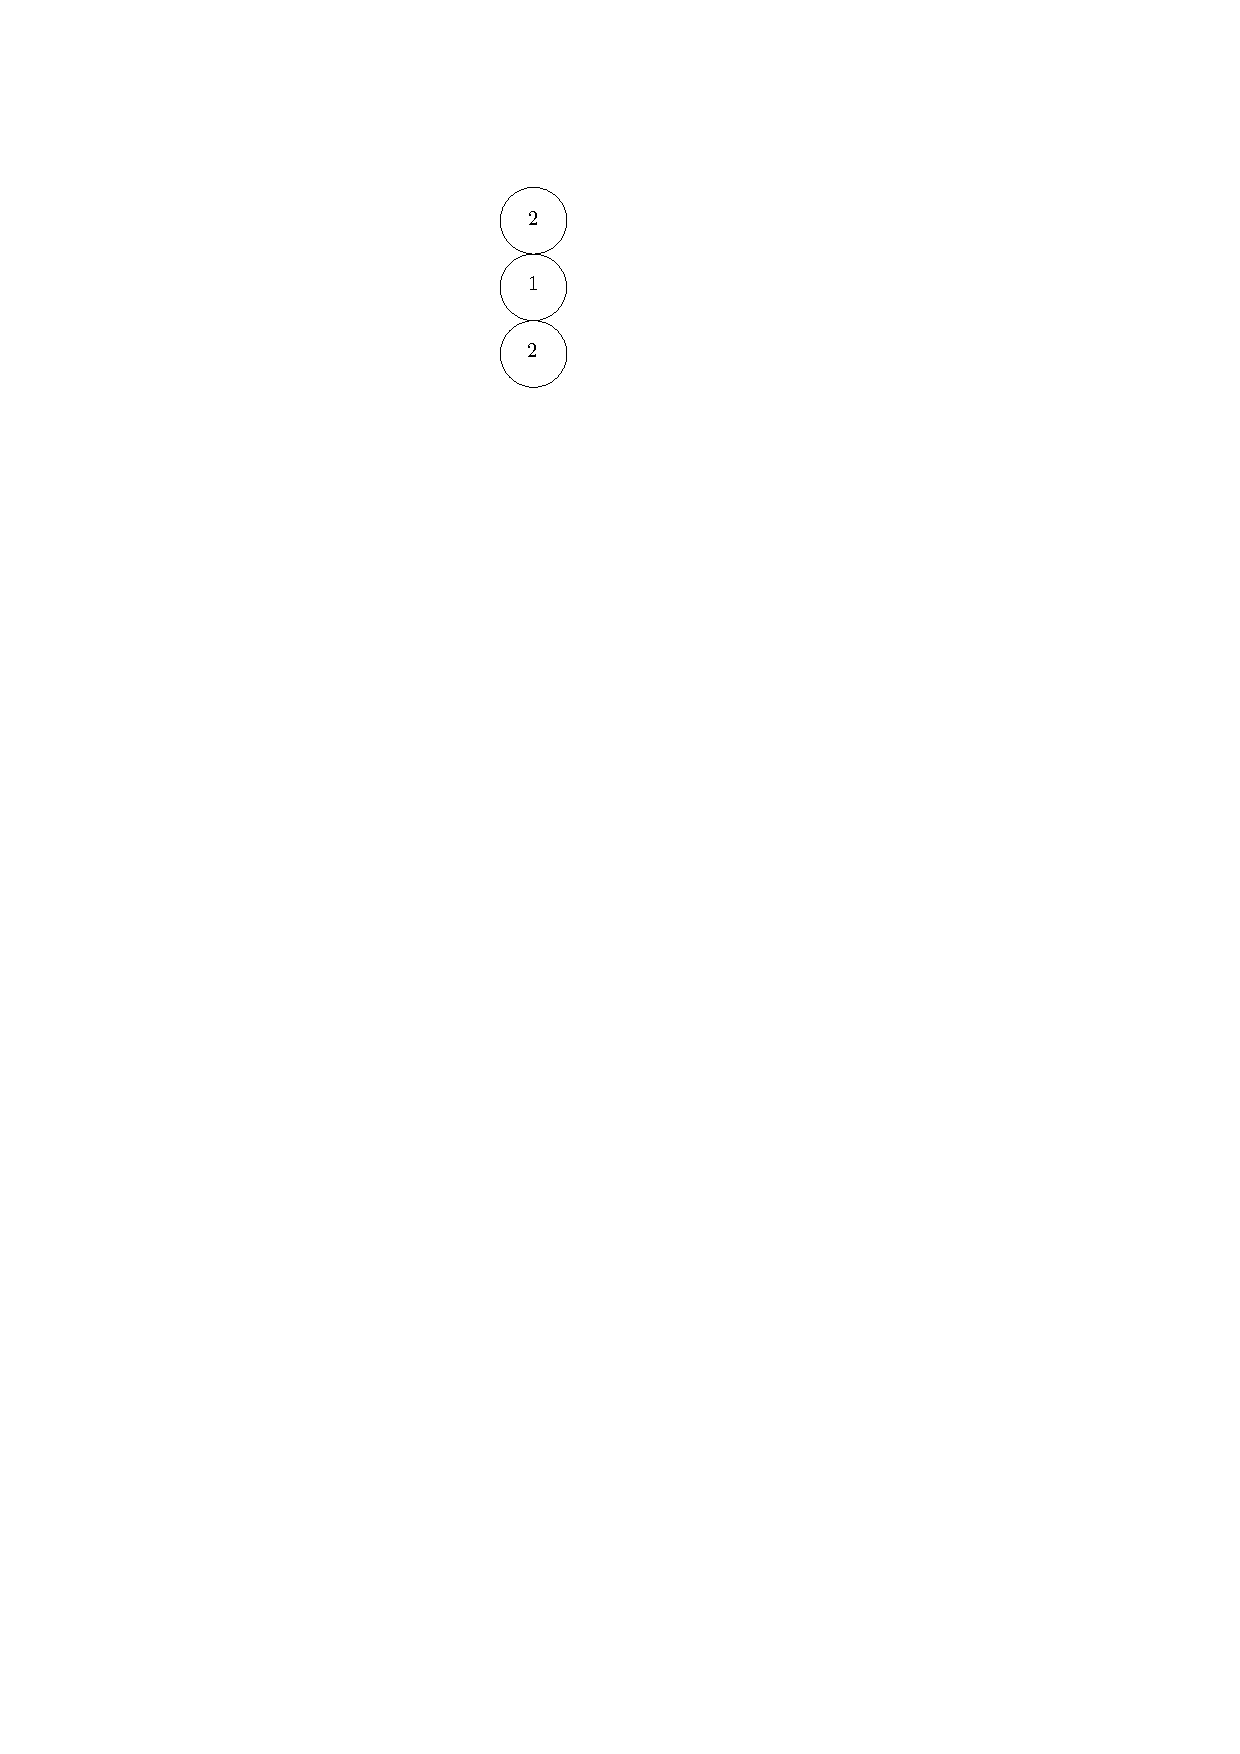
\includegraphics[width=\textwidth]{graphics/degree2arrangement.pdf}
	  \caption{A disk arrangement with two layers of disks}
	  \label{fig:circlePacking2-1}
  \end{subfigure}
  \begin{subfigure}[b]{0.24\textwidth}
	  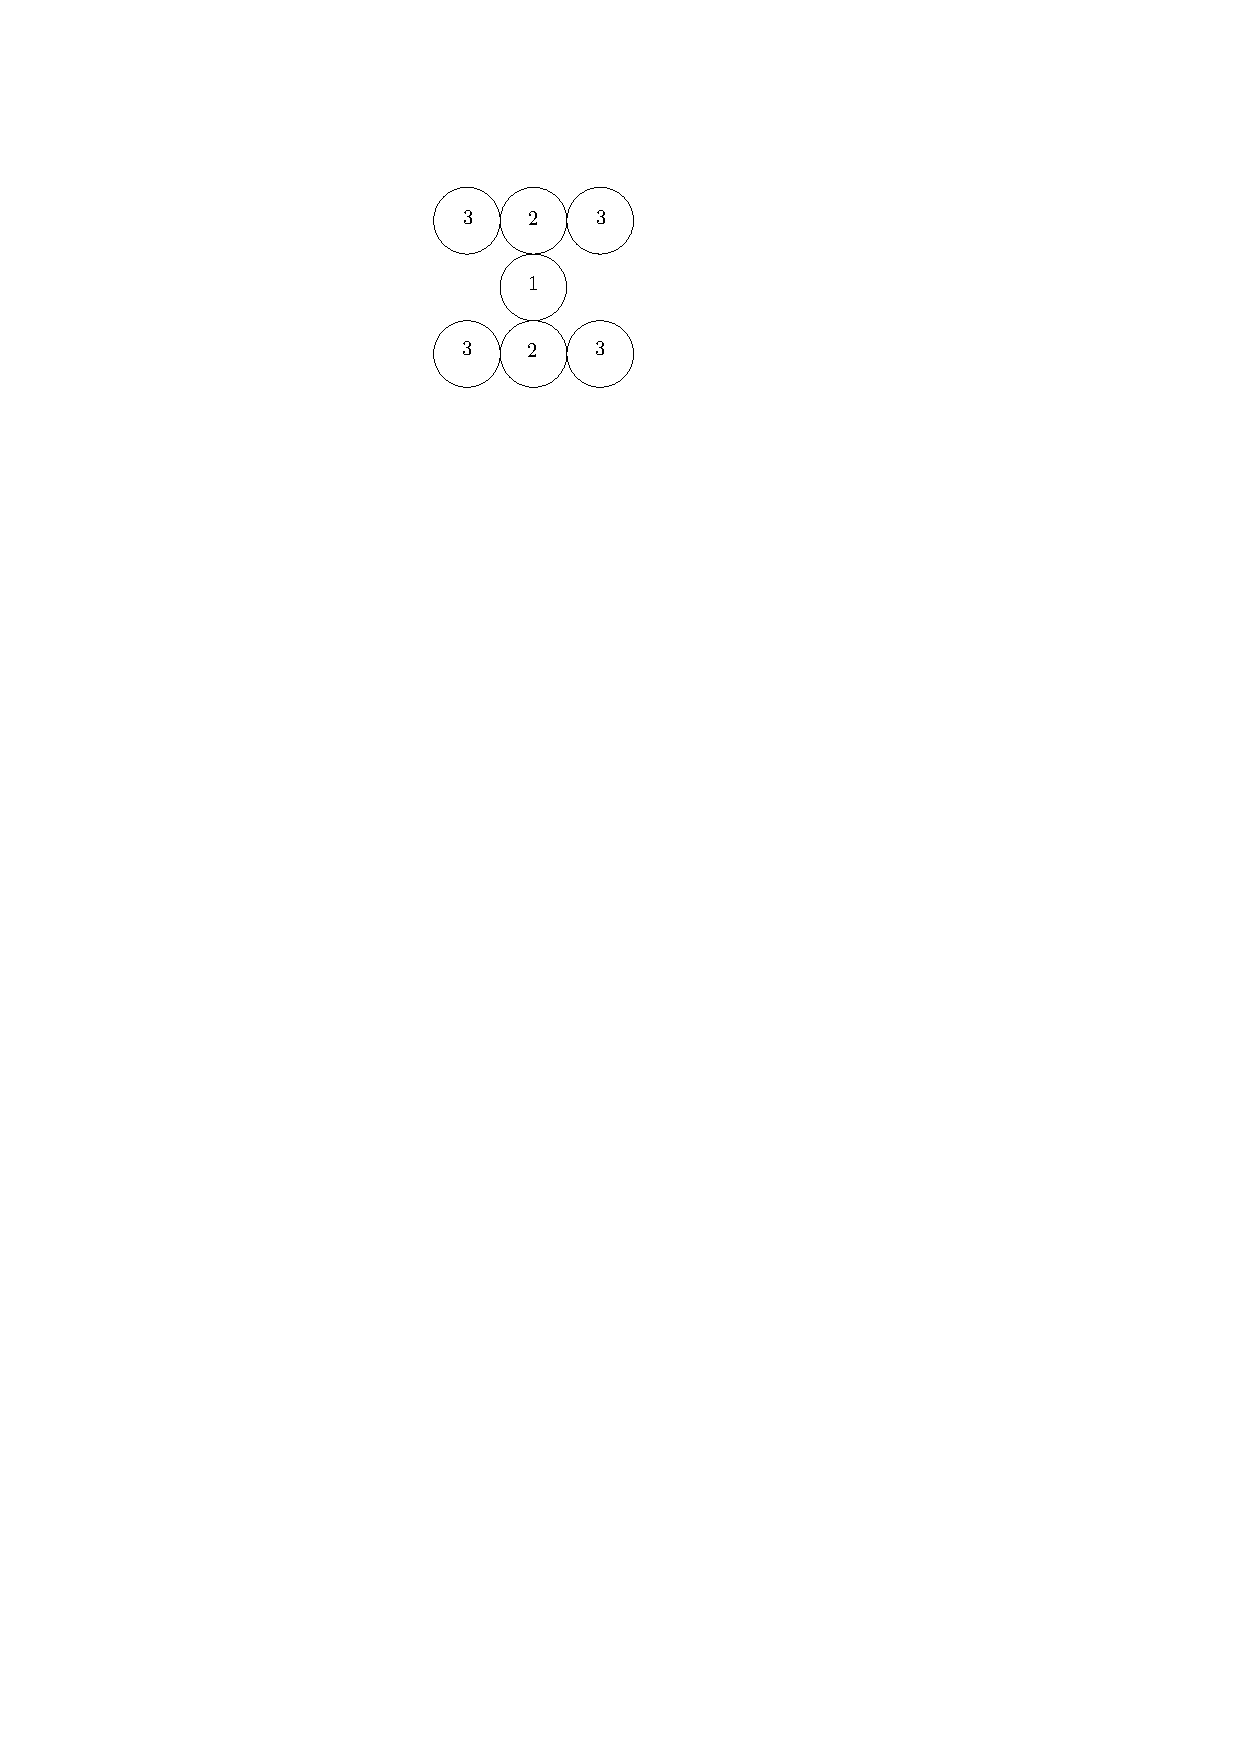
\includegraphics[width=\textwidth]{graphics/degree3arrangement.pdf}
	  \caption{A disk arrangement with three layers of disks}
	  \label{fig:circlePacking2-2}
  \end{subfigure}
  \begin{subfigure}[b]{0.24\textwidth}
	  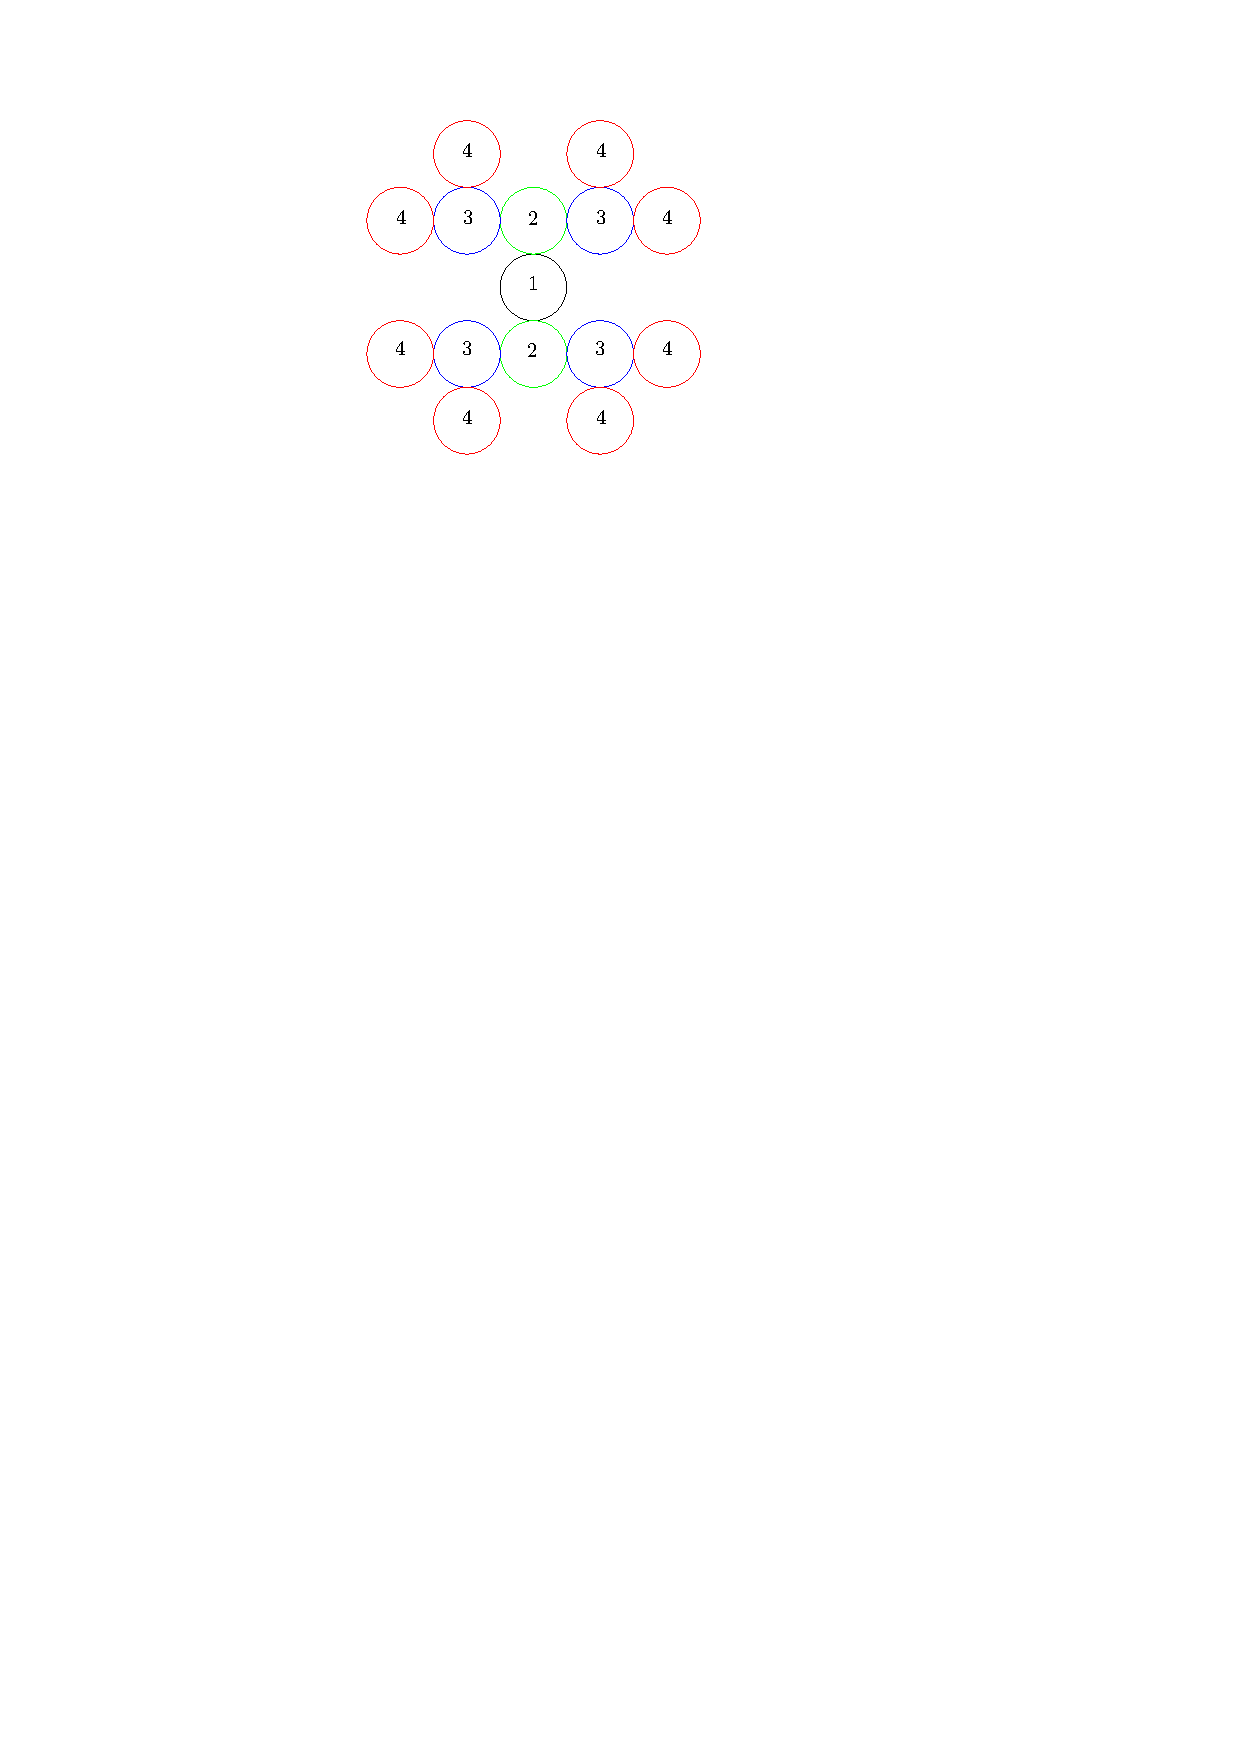
\includegraphics[width=\textwidth]{graphics/degree4arrangement.pdf}
	  \caption{A disk arrangement with four layers of disks}
	  \label{fig:circlePacking2-3}
  \end{subfigure}
  \begin{subfigure}[b]{0.24\textwidth}
	  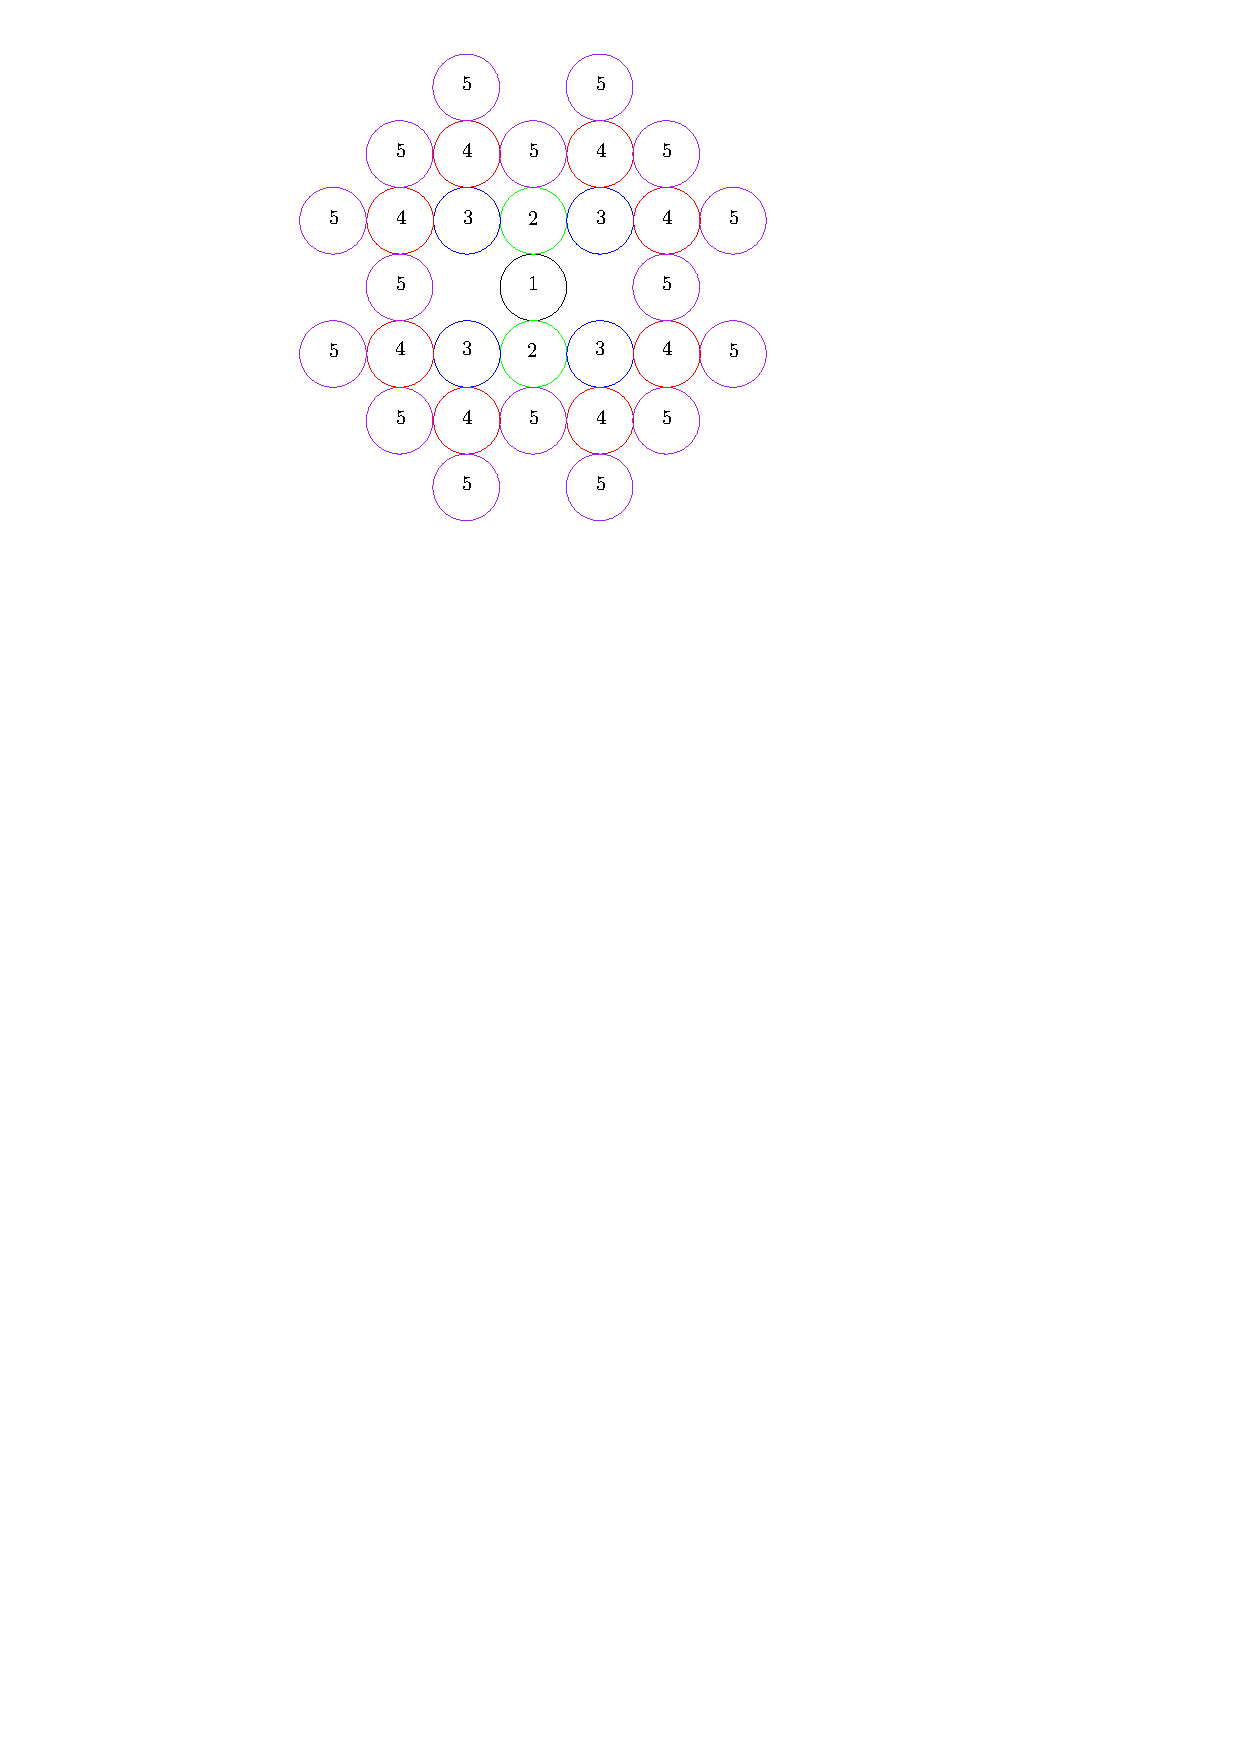
\includegraphics[width=\textwidth]{graphics/degree5arrangement.pdf}
	  \caption{A disk arrangement with five layers of disks}
	  \label{fig:circlePacking2-4}
  \end{subfigure}
\end{center} 
\caption{For $i=2,3,4,5$ the tree $T_i$ is a contact graph of unit disks.}\label{fig:circlePacking-2}
\end{figure}
Figure \ref{fig:circlePacking-2} shows the first four non-trivial trees as a contact graph of unit disks.
Every disk at level up to $i$ is contained in a disk of radius $2\cdot i - 1$ centered at the origin.
The total area of the disk arrangement is $(2\cdot i -1)^2 \cdot \pi$. 
When $i\geq 8$ we have a contradiction.

\begin{figure}[!htbp]
\begin{center}
  \begin{subfigure}[b]{.48\textwidth}
  \begin{center}
	  \includegraphics[scale=.9]{graphics/OrderedDiskArrangementExample1.pdf}
	  \label{fig:circlePacking3-1}
	  \end{center}
  \end{subfigure}
  \begin{subfigure}[b]{0.48\textwidth}
  \begin{center}
	  \includegraphics[scale=.9]{graphics/OrderedDiskArrangementExample2.pdf}	  
	  \label{fig:circlePacking3-2}
	  \end{center}
  \end{subfigure}
  \caption{Consider these two ordered disk arrangements where A and B are in the concentric rings of disks.  The large disks are in contact to A and B respectively.  
  If A and B are adjacent, then there is a restriction of how large the size of the disks can be that are attached to them as seen in on the left.  
  Whereas if A and B are not adjacent in this disk arrangement as shown on the right, the size of the kissing disks could be arbitrarily large.}\label{fig:circlePacking-3}
\end{center} 
\end{figure}

There are instances where a planar graph with weights admits a realization but the cyclic order of neighbors may not be the same as the combinatorial embedding.
Define $G$ as follows: start with a star centered at $C$ and with 6 leafs, $A_1$ through $A_6$; attach two leafs, $B_1$ and $B_2$, to $A_1$ and  $A_2$ respectively (see  Figure \ref{fig:circlePacking-3}).
Let the weight of $C$ be $1+\epsilon$ for sufficiently small $\epsilon > 0$.
The neighbors of $C$ have unit weight.
The weights of the two leaves have weight $\frac{1}{\epsilon}$.  
The right of Figure \ref{fig:circlePacking-3}) shows a realization where $A_1$ and $A_2$ are in opposite position of the counter-clockwise order around $C$.
If $A_1$ and $A_2$ are required to be consecutive in the counter-clockwise order around $C$, there is no realization.

Suppose there is a realization where $A_1, \ldots, A_6$ are in the counter-clockwise order around $C$ (see Figure \ref{fig:DiskArrangement-4}).
If $\epsilon>0$ is sufficiently small, then the centers of of $A_1, \ldots, A_6$ are arbitrarily close to the vertices of a regular hexagon.
Consider the common tangent lines between $A_1$ and $B_1$ and $A_2$ and $B_2$.
The possible position of tangent line between $A_1$ and $B_1$ ranges from the common tangent line of $A_1$ and $A_6$ to the common tangent line of $A_1$ and $A_2$.
Similarly, The possible position of tangent line between $A_2$ and $B_2$ ranges from the common tangent line of $A_2$ and $A_3$ to the common tangent line of $A_1$ and $A_2$.
In any position, the common tangent lines between $A_1$ and $B_1$ and $A_2$ and $B_2$ intersect.
If $\frac{1}{\epsilon}$ is sufficiently large, then the disks $D_1$ and $D_2$ also intersect.
This contradicts that there is a realization.

\begin{minipage}{\linewidth}
\begin{center}
\includegraphics[width=.4\columnwidth]{graphics/orderedPlaneIntersection.pdf}
\end{center}
\captionof{figure}{This example represents a disk arrangement and its contact graph.}
\label{fig:DiskArrangement-4}
\end{minipage}

Figure \ref{fig:circlePacking-3} shows how an ordered contact graph may not be realizable.  
On the left, it shows a limitation on the weights of the disks that are in contact with disks A and B. 
On the right, the figure shows the order where A and B are on opposing ends of the ring of disks and can allow of arbitrary size of weighted disks in contact with A and B.
\section{Configuration Spaces}
\begin{quote}
Just as one can compose colors or forms, so one can compose motions.

{\raggedright{}Alexander Calder, 1933}
\end{quote}


Recall Figure \ref{fig:HingedHaberdasher} illustrating the hinged dissection that formed a square and triangle and several drawings of the hinged dissections that simulate the motion of moving the polygons around the hinge points to form each shape.  The set of all drawings in that motion represents the \textit{configuration space} for that polygonal linkage.  In this section we will formally describe the configuration space for each object we've drawn thus far.

\subsection{Configuration Spaces of Graph Drawings}
Recall that for a graph drawing we have an injective mapping $\Pi : V \mapsto \bbR^{2}$ which maps vertices to distinct points in the plane.  
The mapping $\Pi$ uniquely determines each edge.
An edge $\curlybraces{u,v} \in E$, is mapped to a straight line segment, $c_{u,v}:[0,1]\mapsto \bbR^2$ such that $c_{u,v}(0) = \Pi(u)$ and $c_{u,v}(1) = \Pi(v)$, and does not pass through other vertices.   
Let $\DD_G$ be the set of all drawings of the graph $G$.  
By labelling the vertices of $G$, e.g. $v_1, v_2, \ldots, v_k, \ldots, v_{n}$, we can create a mapping from $\mu: \DD_G \mapsto \bbR^{2\vert V \vert}$ where the coordinates of $\Pi(v_k)$ are the $(2k)^\text{th}$ and $(2k+1)^\text{st}$ coordinates in $\bbR^{2\vert V \vert}$.  
$\mu(\Pi)$ is a configuration.
The configuration space is the set of $\mu(\Pi)$ for all drawings $\Pi$.  

\subsection{Configuration Spaces of Linkages}

Consider drawings of a graph that respects the length assignment.  
A \textit{realization} of a linkage, $(G,\ell)$, is a drawing of a graph, $\Pi$, such that for every edge $\{u,v\} \in E$, $\ell\left( \{u,v\} \right) = \left\vert \Pi(u) - \Pi(v) \right\vert = \left\vert \Pi(v) - \Pi(u) \right\vert$. 
A \textit{plane realization} is a plane drawing with the property, $\ell\left( \{u,v\} \right) = \left\vert \Pi(u) - \Pi(v) \right\vert$.
First let's define the space of realizations for a corresponding linkage, i.e.:
$$P_{(G,\ell)} = \set{\Pi\in \DD_G }{\forall \{u,v\} \in E\text{, }\ell\left( \{u,v\} \right) = \left\vert \Pi(u) - \Pi(v) \right\vert}$$
With respect to $P_{(G,\ell)}$, we can establish a configuration space that allows one to study problems of motion.  
For each vertex of $G$, the drawing of the vertex lies in the plane, i.e. $\Pi(v) \in \bbR^2$.  
By enumerating each vertex of $G$, e.g. $v_1, v_2, \ldots, v_k, \ldots, v_{n}$, we can create a mapping from $\mu: P_{(G,\ell)} \mapsto \bbR^{2\vert V \vert}$ where the corresponding coordinates of $\Pi(v_k)$ are in the $(2k)^\text{th}$ and $(2k+1)^{st}$ coordinates in $\bbR^{2\vert V \vert}$.  
The configuration space is $\mu\lr{P_{(G,\ell)}}$.  

Using standard definitions from real analysis, we can begin to pose problems about linkages with respect to a corresponding configuration space.  
A continuous function $\gamma: [0,1]\mapsto \mu\lr{P_{(G,\ell)}}$ is a path from a realization $\gamma(0)$ to another realization $\gamma(1)$.
$\gamma$ can be thought of as an animation of drawings that starts at $\gamma(0)$ and ends at $\gamma(1)$.  
Any two realizations in the same path-connected component can be animated from one to the other continuously.
The Carpenter's Rule states that every realization of a path linkage can be continuously moved (without self-intersection) to any other realization \cite{CDR03,Str05}.
To ask if $\mu\lr{P_{(G,\ell)}}$ is a connected space, is to ask if $\mu(P)$ is connected in $\bbR^{2\vert V \vert}$.
In other words, the realization space of such a linkage is always path-connected.

\begin{figure}[!htbp]
\begin{center}
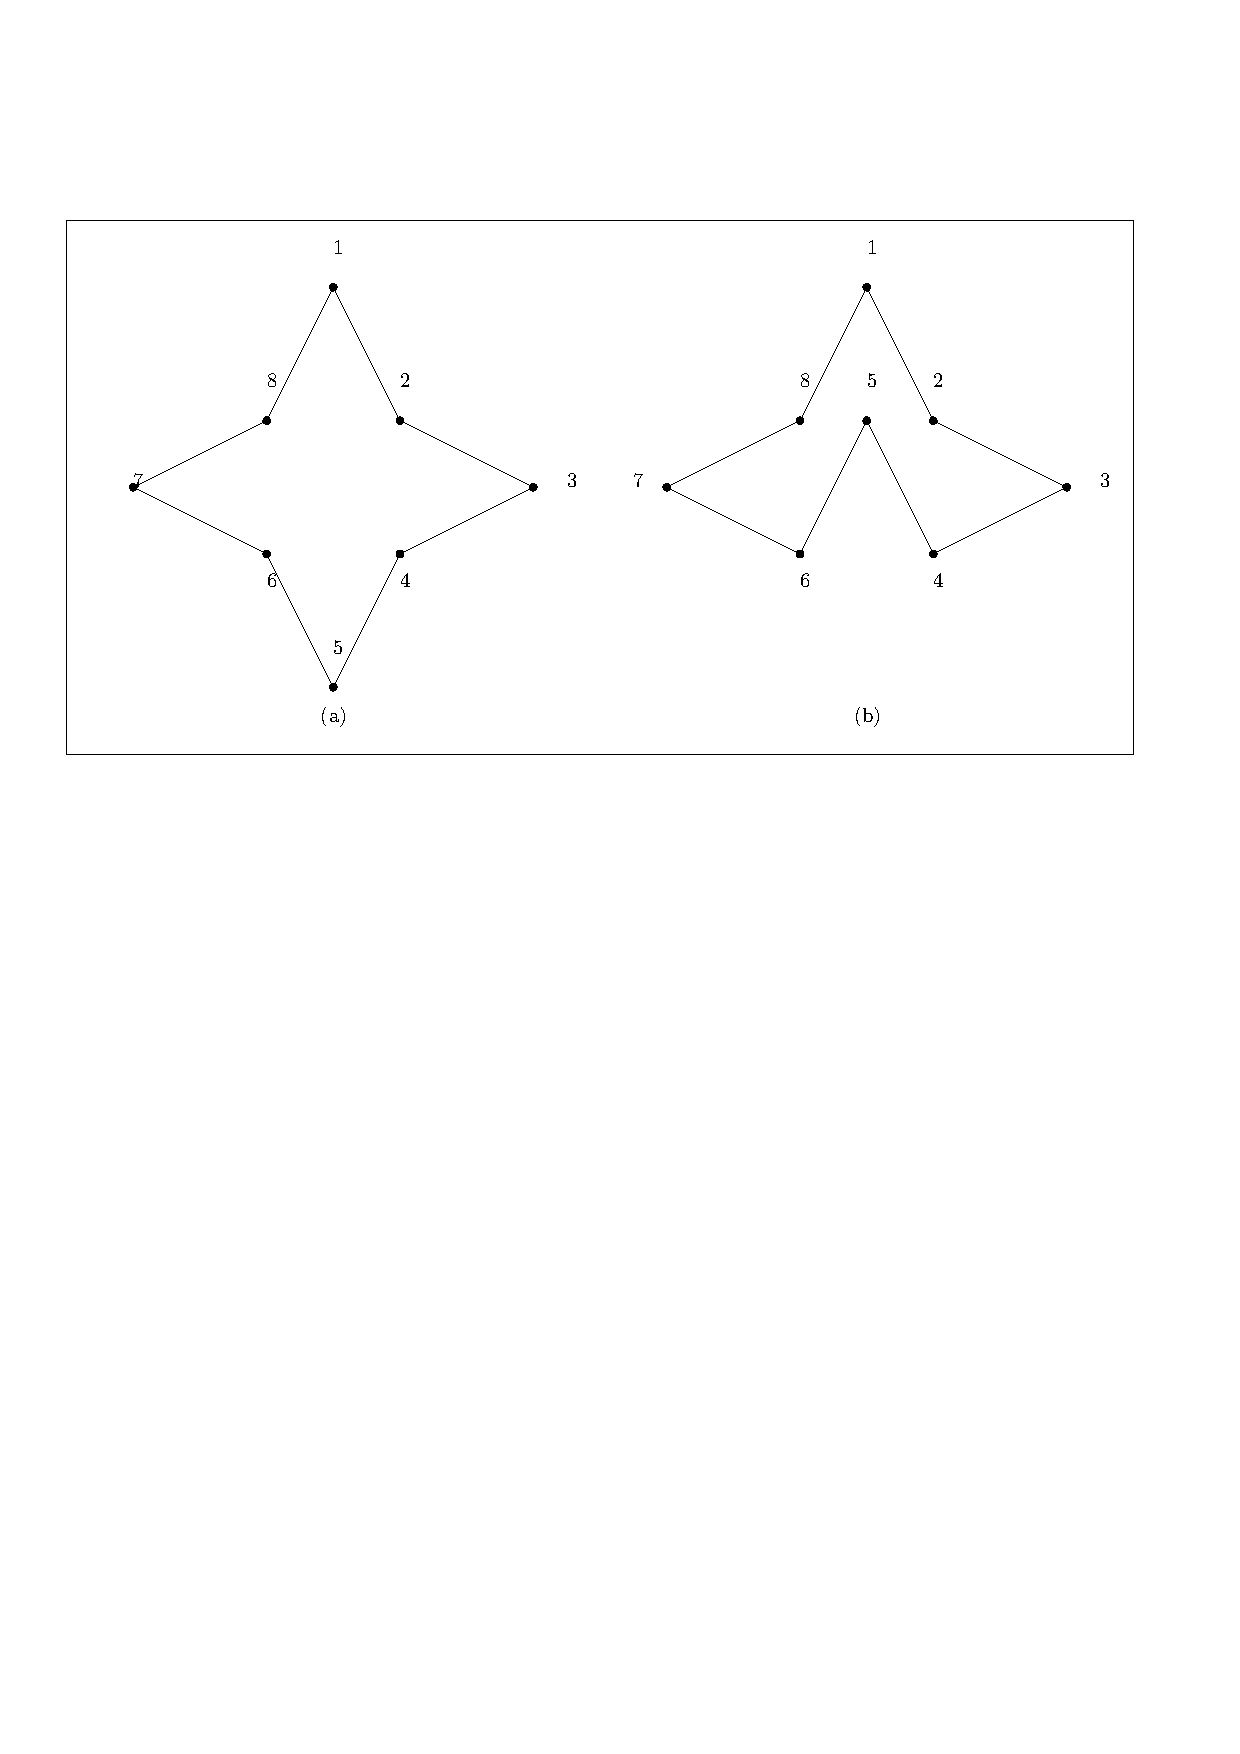
\includegraphics{graphics/twoEmbeddingsOfSameLinkage.pdf}
\end{center} 
\caption{(a) and (b) show a linkage in two embeddings.  Any realization of a path can be continuously moved without self-intersection to any other realizations.}
\label{fig:twoEmbeddingsOfSameLinkage.pdf}
\end{figure}

\subsection{Configuration Spaces of Polygonal Linkages}
The placement of a polygon is described by an isometry of Euclidean plane.
An isometry is a composition of a translation, a rotation, and a possible reflection.
As such, the isometry can be described as three parameters: $\lr{a,b,\theta}$ where $(a,b)$ is a translation vector; if $\theta \geq 0$, it describes a counter-clockwise rotation by $\theta$ and if $\theta < 0$, it describes a reflection in the x-axis followed by a counter-clockwise rotation $\theta$.
For $m$ polygons there will be $3 m$ parameters.
Recall a realization of a polygonal linkage is an interior-disjoint placement of congruent copies of the polygons in $\PP$ such that the copies of a hinge are mapped to the same point (e.g., Figure \ref{fig:linkage-1}).
First consider the set of all realizations for the polygonal linkage $\left(\PP,\HH\right)$ and call it $P$.  
$\mu:P \mapsto \bbR^{3m}$ where $m$ is the number of polygons in $\PP$ is the configuration space function and the configuration space is the set $\mu(P)$. 

 \subsection{Configuration Spaces of Disk Arrangements}
The placement of a polygon is described by an isometry of Euclidean plane.
An isometry is a composition of a translation, a rotation, and a possible reflection.
As such, the isometry can be described as three parameters: $\lr{a,b,\theta}$ where $(a,b)$ is a translation vector; if $\theta \geq 0$, it describes a counter-clockwise rotation by $\theta$ and if $\theta < 0$, it described a reflection in the x-axis followed by a counter-clockwise rotation $\theta$.
For $m$ polygons there will be $3 m$ parameters.
Recall a realization of a polygonal linkage is an interior-disjoint placement of congruent copies of the polygons in $\PP$ such that the copies of a contact are mapped to the same point (e.g., Figure \ref{fig:linkage-1}).
First consider the set of all realizations for the polygonal linkage $\left(\PP,\HH\right)$ and call it $P$.  
$\mu:P \mapsto \bbR^{3m}$ where $m$ is the number of polygons in $\PP$ is the configuration space function and the configuration space is the set $\mu(P)$. 

\begin{figure}[!htbp]
\begin{center}
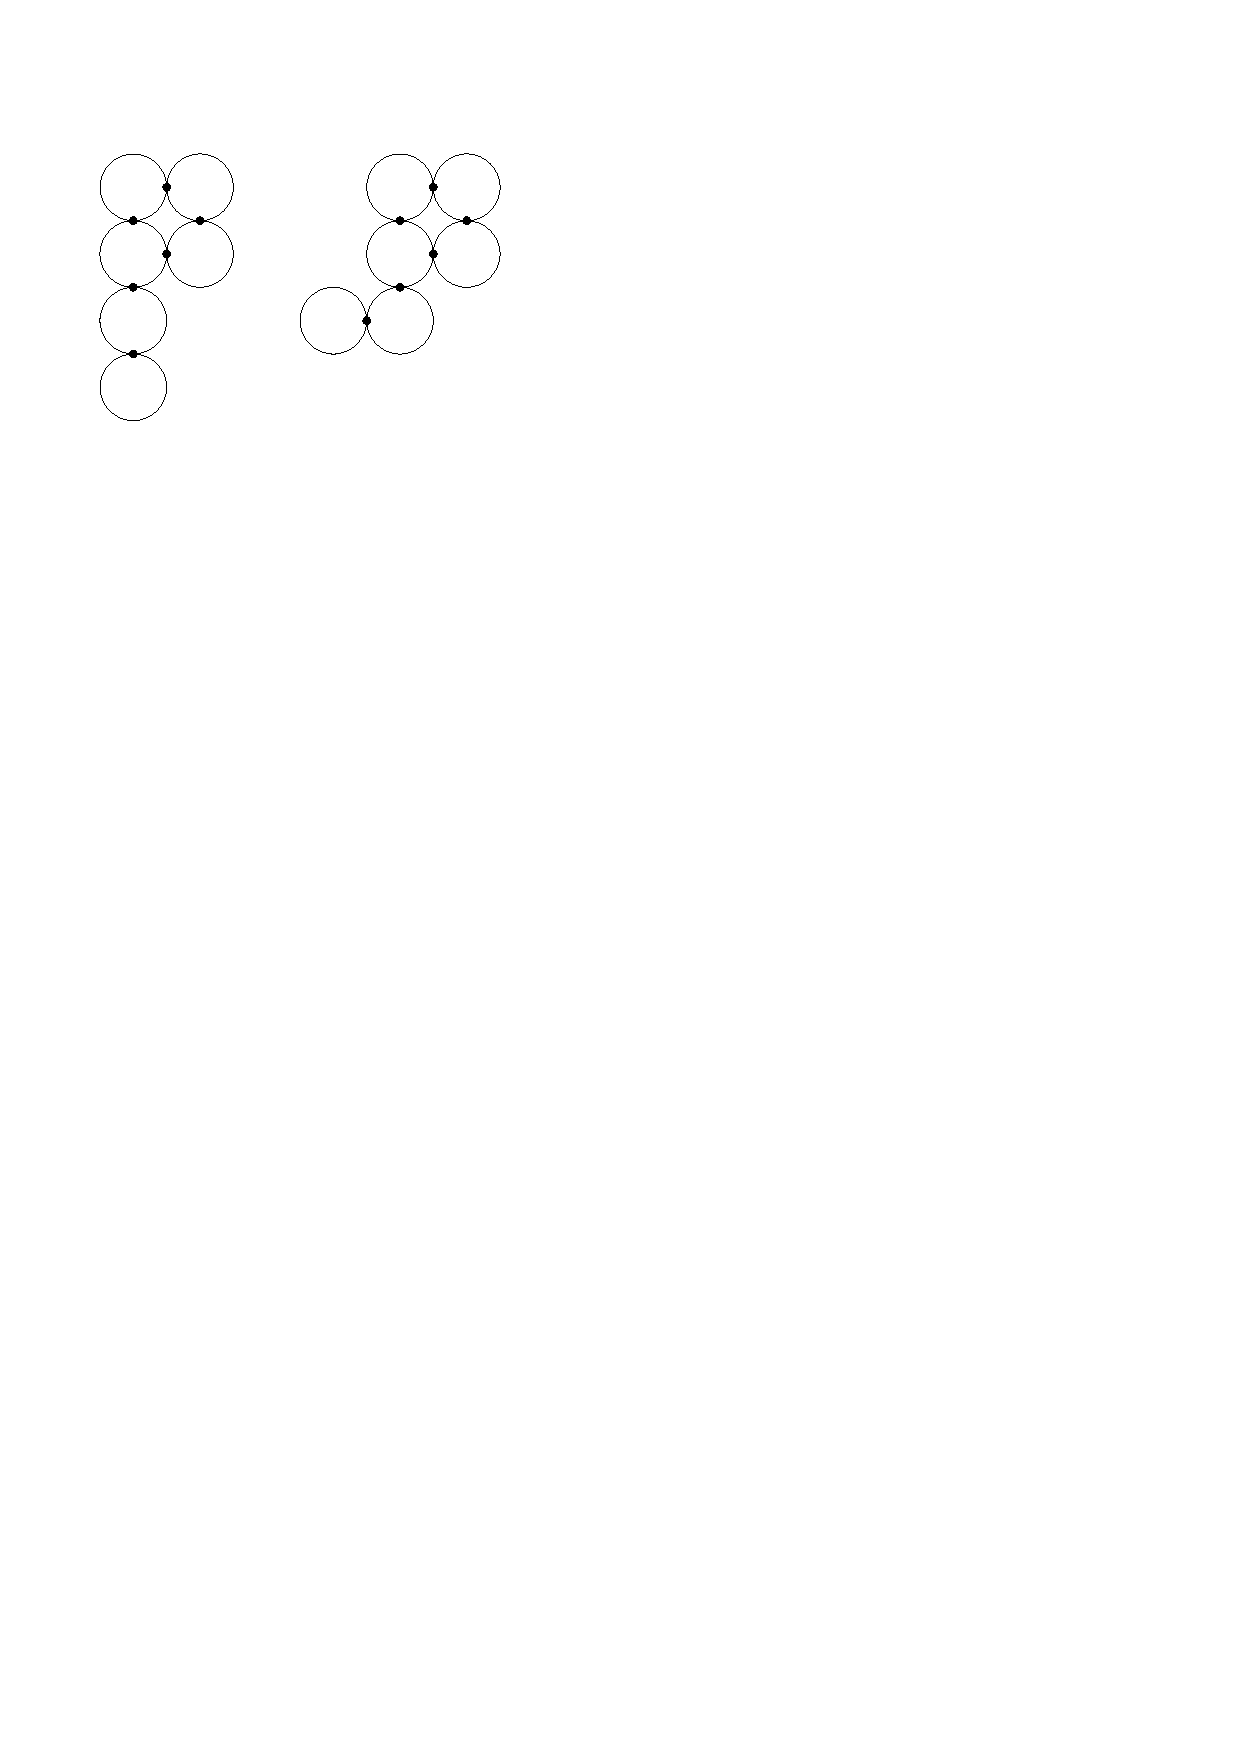
\includegraphics[scale=.75]{graphics/DiskPackingReconfiguration.pdf}
\end{center} 
\caption{An example of a disk arrangement where $A$ and $B$ have a large range of freedom to move around.  $C$, $D$, $E$, and $F$ are limited in their range of motion to due to their contact points.}
\label{fig:configuration-5}
\end{figure}

Consider the set of realizations $P$ for a given disk arrangement $\DD = \left\lbrace D_i \right\rbrace_{i=1}^n$.  For any realization $R \in P$, there exists a corresponding contact graph, $C$.  The configuration spaces of $\DD$ are sets of $R \in P$ that are classified by the equivalent contact graphs, i.e. if $R_1$, $R_2 \in P$ and their corresponding contact graphs $C_1$ and $C_2$ have a graph isomorphism, $\phi$, then $R_1$ and $R_2$ belong to the same configuration space.



\section{Algorithm Complexity}
\textit{Algorithms} are a list of instructions executed with a given input.  
The efficiency of an algorithm can be measured in terms of the amount of resources it uses such as time, memory, and power.
Ideally, a desirable algorithm would primarily have a small run time and secondarily utilize a small amount of resources.

The time and space used by an algorithm is measured with units defined by a model of computation.
The actual running time of an algorithm depend on a variety of factors for example: the processor, the hardware, the temperature, etc.
Mathematical models of computation have been developed to measure running time of algorithms independent of the machine it runs on.
One of the oldest and most popular models is the random access machine (RAM) model.
RAM measures the unit of space in the number of words used where each word can store an arbitrary integer.
In the real RAM, each word can store an arbitrary real number.
The units of time is measured in the number of arithmetic operations and number of memory accesses (read or write). 

The \textit{running time} of an algorithm on a given input, is the time it takes to terminate.% an algorithm with the input. 
The \textit{worst-case} running time is the largest running time over all inputs of a given size $N$.  
It is a function of $N$, it is usually monotonically increasing function since larger inputs tend to take more time to process.
The key parameter of the efficiency of an algorithm is the growth rate of its worst case running time in terms of $N$.
An algorithm is said to be \textit{efficient} if the time needed to perform the list of instructions can be determined from a polynomial. 
Devising an efficient algorithm for a given problem is often a difficult task.

The growth rate of running times are typically compared up to constant vectors.
Let $f$ and $g$ be defined on some subset of $\bbR$.  
$f(x) = O\left(g(x)\right)$ if and only if there exists a constant $M$ and $x_0$ such that $$\left\vert g(x)\right\vert \leq M \left\vert f(x) \right\vert$$
for all $x \geq x_0$.

\subsection{Complexity Classes}
Problems can be categorized by their running times.
Each algorithm computes a function $f(I)$ on an input $I$, however many different algorithms can compute the same function.
Algorithms are differentiated by their running times but the function is characterized by the fastest algorithm that can compute it.
A problem can be formulated as follows, given input $I$ find $f(I)$.

Problems can be categorized into complexity classes based on the fastest algorithms that solve them.
The class of problems that can be solved in polynomial running time is called the \textit{polynomial time} class, $\P$.

A second property of problems is whether its solution can be verified efficiently.  
This property is independent of whether it can be solved efficiently.  
$B$ is said to be an \textit{efficient certifier} for a problem $X$  if the following properties hold:
\begin{itemize}
\item[(i)] $B$ is a polynomial-time algorithm that takes two inputs $s$ and $t$.
\item[(ii)] There exists a polynomial function $p$ such that for every string $s$, we have $s \in X$ if and only if there exists a string $t$ such that $\vert t \vert \leq p\left( \vert s \vert \right)$ and $B(s,t) = \text{`yes'}$.
\end{itemize}

The class of problems which have an efficient certifier is said to be the \textit{non-deterministic polynomial time} class, $\NP$. 
We continue with the definitions for $\NP$-hard and $\NP$-complete.
A problem is $\NP$-hard if every problem in $\NP$ can be reduced to it in polynomial time.
A \textit{polynomial time reduction} is when arbitrary instances of problem $Y$ be solved using a polynomial number of standard computational steps, plus a polynomial number of calls to a black box that solves problem $X$, i.e. $Y$ is reduced in polynomial time to $X$.
A problem is $\NP$-complete if it $\NP$ and $\NP$-hard, i.e. $\NP$-complete = $\NP \cap \NP$-hard.

\subsection{RSA Cryptosystem}
Cryptography is the study of secure communication between parties in an untrusted or insecure communication channel.
Cryptography has three primary purposes for secure communications: provide confidentiality, authenticate entities, and verification of data.
Modern cryptography is based on hard math problems such as integer factorization, discrete logarithmic problem, and pre-image problems. 
Hard math problems are not found in $\P$ and found in $\NP$.
In most forms of modern cryptography, \textit{keys}, are data parameters used to form function outputs for the use in a communication channel.
There are three common types of keys in cryptography:
\begin{enumerate}
\item A \textit{secret key} is known by certain entities.  Typically a secret key is used by entities to encrypt and decrypt data that is communicated over an untrusted channel.  Secret keys require a secure channel to exchange between all entities.
\item When there are no means to exchange secret keys, one can use a private and public key scheme.
A \textit{public key} is a key that can be shared with any entity, i.e. trusted and untrusted entities can know it.
The \textit{private key} is a key that is kept to one entity. It is treated like a secret key and should only be known to that entity.
\end{enumerate}
A \textit{cryptosystem} is a suite of algorithms used to establish secure communication channel between parties. 
The RSA cryptosystem is the first practical cryptosystem in modern cryptography that allows for encryption of data (confidentiality), authentication of entities, and verify message integrity using just one underlying hard math problem, integer factorization.

RSA is named after its second inventors, Ron Rivest, Adi Shamir, and Leonard Adelmen.
These three individuals devised and published the algorithm in 1977.
The original inventor of RSA was Clifford Cocks in 1973 however, it was only known to the public since 1997 that Clifford Cocks was the original inventor because his was was classified by Government Communication Headquarters, an intelligence agency of the United Kingdom.

For the RSA cryptosystem, we first want to pose the communication security problem.  
Suppose we have two entities, Alice and Bob, that wish to communicate over an insecure channel.
Should Alice and Bob agree to using RSA, each entity will have a pair of keys, a private key and a public key.
Most implementations of RSA use the following key derivation \cite{rivest1978method}:
\begin{enumerate}
\item Let $n=p\cdot q$ where $p$ and $q$ are randomly chosen prime numbers.
\item Choose an integer $e$ such that $1 < e \leq \phi (n)$ and $gcd\lr{e,\phi\lr{n}}=1$ where $\phi$ is the Euler totient function.
\item Let $d \equiv e^{-1} \mod \phi(n)$.
\end{enumerate}
The RSA cryptosystem is based around the following formula:
$$\left(m^e\right)^d \mod n= \left(m^d\right)^e \mod n\equiv m \mod n$$
where we have natural numbers $e$, $d$, $m$, and $n$, such that $m < n$ and $gcd(m,n)=1$.


If Alice derives a public and private key in the manner described, her public key is $(n,e)$ and her private key is $d$.
Suppose Bob wants to send Alice a message $M$.  
Bob will represent $M$ in binary form, $m$.  
Alice sends her public key $(n,e)$ to Bob and keeps her private key $d$ secret.  
If $gcd(m,n)\neq 1$, then Bob modifies $m$ by padding $m$ with additional digits so that $m$ becomes co-prime with $n$.
There are efficient padding schemes to modify $m$ such that $m$ and $n$ are co-prime \cite{jonsson2003public}.
Bob sends the following value, $c$, to Alice:
$$c \equiv m^e \mod n$$
$c$ is said to be a ciphertext.
Alice can decrypt the ciphertext and recover $m$ by computing:
$$ m \equiv c^d \mod n = \lr{m^e}^d \mod n$$

The RSA cryptosystem is based on integer factorization and the RSA problem, given $n$ where $n=p\cdot q$ where $p$ and $q$ are prime numbers, find $p$ and $q$.
For sufficiently large integers, factorization and the RSA problem becomes very difficult.  
If there were an algorithm that solved integer factorization in polynomial time, then one can also solve the RSA problem as well.
Suppose a third party listens into the conversation and knows Alice's public key $(n,e)$ and the ciphertext $c$.
If the the third party can factor $n = p\cdot q$ then the attacker can computer $\phi(n)$ and compute $d \equiv e^{-1} \mod \phi(n)$ using the extended Euclidean algorithm.
Once they have $d$, the attacker can compute $m \equiv c^d \mod n$.

Currently, the most efficient factorization algorithm is the general number sieve algorithm \cite{lenstra1993number}.
It's an exponential running time algorithm.
If a polynomial running time algorithm for integer factorization existed, it would allow for compromise of security that is provided to communicating parties by the RSA cryptosystem.
It would allow for a reduction of the integer factorization problem, a problem that exists in $\NP$ but not $\P$.
The algorithm would allow for an adversary to attack RSA \cite{menezes1996handbook} in polynomial time.



\section{Satisfiability}\label{sec:logic}
Let $x_1, \ldots, x_n$ be Boolean variables.  A Boolean formula is a combination of conjunction, 
disjunctions, and negations of the Boolean variables $x_1,  \ldots, x_n$.   
A \textit{clause} is a disjunction of distinct literals.  
A \textit{literal} is a variable or a negated variable, $x_i$ or $\bar{x}_i$, for $i = 1,\ldots,n$. 
A Boolean formula is \textit{satisfiable} if one can assign true or false value to each variable so that the formula is true. 
It is known that every Boolean formula can be rewritten in \textit{conjunctive normal form} (CNF), a conjunction of clauses, via DeMorgan's law and distributive law.   
Furthermore, it is also known that every Boolean formula can be written in CNF such that each clause has exactly three literals. 
This form is called 3-CNF.  
For example, consider the clause $A \lor B \lor C \lor D \lor E$. 
This clause can be rewritten in 3-CNF form as $(A \lor B \lor x_1) \land (\lnot x_1 \lor C \lor x_2) \land (\lnot x_2 \lor D \lor E)$ where $x_1$ and $x_2$ are literals that allow us to form 3-CNF clauses.
Here are the problem statements for satisfiability:
%\textit{3-SAT problem}.
\begin{prob}[Satisfiability Problem (SAT)]\label{prob:Satisfiability-1}%Problem/Question
Given a Boolean formula, is it satisfiable? \cite{skiena2009algorithm}
\end{prob} 
\textit{Brute force} is when an algorithm tries all possibilities to see if any formulates a satisfiable solution.
It is clear that SAT is decidable in exponential time by testing all possibilities.
This is called a brute force solution.
It is not known whether SAT admits a polynomial time solution, that is whether it is in $\P$. 
\begin{prob}[3-SAT Problem]
Given a Boolean formula in 3-CNF, is it satisfiable?
\end{prob}
The problems we focus on in this thesis have a geometry.  
A special geometric 3-SAT problem is that Planar 3-SAT Problem.   
Given a 3-CNF Boolean formula, $\Phi$, with $n$ variables and $m$ clauses, 
we define the \textit{associated graph} $A(\Phi)$ as follows: the vertices correspond to the variables and clauses in $\Phi$.   
We place an edge in the graph if variable $x_i$ appears in clause $C_j$.

  \begin{figure}[htbp]
	\centering
	\includegraphics[width=0.7\columnwidth]{graphics/fig-assoc-hex}
	\caption{Left: the associated graph $A(\Phi)$ for a Boolean formula $\Phi$.
Right: the schematic layout of the variable, clause, and transmitter gadgets in the auxiliary construction showing in Section \ref{sec:auxiliaryConstruction}}
	\label{fig:assoc}
\end{figure} 
\begin{prob}[Planar 3-SAT]
 Given a Boolean formula $\Phi$ in 3-CNF such that its associated graph is planar, decide whether it 
is satisfiable is a \textit{3-SAT problem}.
\end{prob}
Figure \ref{fig:assoc} is associated to a family of Boolean formulas.  
One such associated Boolean formula is:
$$(x_1 \lor x_3 \lor \lnot x_5) \land (\lnot x_1 \lor \lnot x_2 \lor x_3) \land (\lnot x_3 \lor x_4 \lor \lnot x_5) \land (x_2 \lor x_4 \lor \lnot x_5) \land ( \lnot x_1 \lor x_2 \lor x_5)$$
Note that the figure establishes an edge relation between variables and clauses whereas the clauses in Boolean formulas do not have variables but literals of variables.
\begin{prob}[Not All Equal 3 SAT Problem (NAE3SAT)]\label{prob:Satisfiability-2}%Problem/Question
Given a Boolean formula in 3-CNF, is it satisfiable so that each clause contains a 
true and a false literal?
\end{prob}

Problems \ref{prob:Satisfiability-1}---\ref{prob:Satisfiability-2} are known to be NP-hard and are often used to show other problems are NP-hard as well \cite{lichtenstein1982planar,karp1972reducibility}.

\section{Contribution}
% \abstract{
% This thesis addresses the computational complexity of two geometric
% problems, motivated by applications in protein folding. In both
% problems, we are given $n$ geometric objects together with a local
% combinatorics (neighborhood relations specified by a contact graph or a
% hinge graph), and ask whether these objects have a nonoverlapping
% placement in Euclidean plane that \emph{realizes} the given combinatorial
% structure. In the first problem, the geometric objects are simple
% polygons and their local structure is specified by flexible hinges
% attached to the boundaries of two or more polygons. In the second
% problem, the geometric objects are circular disks and their local
% structure is characterized by pairs of disks that must be in contact. It
% was previously known that the realizability of these geometric
% structures is NP-hard when their contact graph contains cycles (e.g.,
% tiling or disk packing). We prove that these problems remain NP-hard
% when the contact graph is a treed. We give polynomial-time reductions
% from known NP-hard problems: Planar 3-SAT (P3SAT) and Not-All-Equal
% 3-SAT (NAE3SAT).
% }
The \emph{realizability} problem for a polygonal linkage asks whether a given polygonal linkage has 
a realization (resp., orientated realization). 
For a weighted planar graph, it asks whether the graph is the ordered contact graph of some disk arrangement with specified radii. 
These problems, in general, are known to be NP-hard. 
Specifically, it is NP-hard to decide whether a given planar (or plane) graph can be embedded in $\RR^2$ with given edge lengths~\cite{CDD+10,EW90}. 
Since an edge of given length can be modeled by a suitably long and skinny rhombus, the realizability of polygonal linkages is also NP-hard. The recognition of the contact graphs of unit disks in the plane (a.k.a. coin graphs) is NP-hard~\cite{BK98}, and so the realizability of weighted graphs as contact graphs of disks is also NP-hard.  
However, previous reductions crucially rely on configurations with high genus: the planar graphs in~\cite{CDD+10,EW90} and the coin graphs in~\cite{BK98} have many cycles.

In this thesis, we consider three realizability problems when the union of the polygons 
(resp., disks) in the desired configuration is simply connected (i.e., contractible). That is, the 
contact graph of the disks is a tree, or the ``hinge graph'' of the polygonal linkage is a tree (the 
vertices in the \emph{hinge graph} are the polygons in $\PP$, and edges represent a hinge between 
two polygons). Our main result is that realizability remains NP-hard when restricted to simply 
connected structures.
 
\begin{thm}\label{thm:hinge2}
It is strongly NP-hard to decide whether a polygonal linkage whose hinge graph is a \textit{tree} can be realized.
\end{thm}
\begin{thm}\label{thm:hinge3}
It is strongly NP-hard to decide whether a polygonal linkage whose hinge graph is a \textit{tree} can be realized with fixed orientation.
\end{thm}

Our proof for Theorem \ref{thm:hinge3} is a reduction from {\sc Planar-3-SAT} (P3SAT): decide whether a given Boolean formula in 3-CNF with a planar associated graph is satisfiable. 
Our proof for Theorem \ref{thm:hinge2} is a reduction from {\sc Not-All-Equal-3-SAT} (NAE3SAT): decide whether a given Boolean formula in 3-CNF  is it satisfiable so that each clause contains a true and a false literal?

\begin{thm}\label{thm:disk}
It is NP-Hard to decide whether a given ordered tree with positive vertex weights is the contact graph of a disk arrangements with specified radii.
\end{thm}

The unoriented versions, where the underlying graph (hinge graph or contact graph) is a tree can 
easily be handled with the logic engine method (Section \ref{sec:logic}). We prove 
Theorem \ref{thm:hinge3} for \emph{oriented} realizations with a reduction from {\sc Planar-3SAT} 
(Section \ref{sec:hinge}), and then reduce the realizability of ordered contact trees to the 
oriented realization of polygonal linkages by simulating polygons with disk arrangements
(Chapter \ref{chp:disk}).

\section{Related Work and Results}
Previous research has established NP-hardness in several easy cases, but realizability for simply connected structures remained open. Polygonal linkages (or body-and-joint frameworks) are a generalization of classical linkages (bar-and-joint frameworks) in rigidity theory. A linkage is a graph $G=(V,E)$ with given edge lengths~\cite{CD-ch9}. A realization of a linkage is a (crossing-free) straight-line embedding of $G$ in the plane. Based on ideas developed by Bhatt and Cosmadakis~\cite{BC87}, who proved that the realizability of linkages is NP-complete on the integer grid, the \emph{logic engine} method~\cite{BET+99,EW96,FHW97,HK01} has become a standard tool for proving NP-hardness in graph drawing. The logic engine is a graph composed of rigid 2-connected components, where two possible realizations of a 2-connected component encode a binary variable.

However, the logic engine method is \textit{not} applicable to problems with fixed embedding or orientation, where the circular order of the neighbors of each vertex is part of the input. Cabello et al.~\cite{CDR07,EW90} used a significantly more elaborate reduction to show that the realizability of 3-connected linkages (where the orientation is unique by Whitney's theorem~\cite{W33}) is NP-hard. This problem is efficiently decidable, though, for near-triangulation~\cite{CDR07,BV96}.

Note that every \emph{tree} linkage can be realized in $\RR^2$ with almost collinear edges. According to the celebrated \emph{Carpenter's Rule Theorem}~\cite{CDR03,Str05}, every realization of a path (or a cycle) linkage can be continuously moved (without self-intersection) to any other realization. In other words, the realization space of such a linkage is always connected. However, there are trees of maximum degree 3 with as few as 8 edges whose realization space is disconnected~\cite{BCD+09}; and deciding whether the realization space of a tree linkage is connected is PSPACE-complete~\cite{AKR+04} (Earlier, Reif~\cite{Rei79} showed that it is PSPACE-complete to decide whether a polygonal linkage can be moved from one realization to another among polygonal obstacles in $\RR^3$.).  
Cheong et al.~\cite{CdG+07} consider the ``inverse'' problems of introducing the minimum number of point obstacles to reduce the configuration space of a polygonal linkage to a unique realization.

Connelly et al.~\cite{CDD+10} showed that the Carpenter's Rule Theorem generalizes to certain polygonal linkages obtained by replacing the edges of a path linkage with special polygons (called \emph{slender adornments}). Our Theorem~\ref{thm:hinge2} indicates that if we are allowed to replace the edges of a linkage with arbitrary convex polygons, then deciding whether the realization space is empty or not is already NP-hard.

Recognition problems for intersection graphs of various geometric object have a rich history~\cite{HK01}.
Breu and Kirkpatrick~\cite{BK98} proved that it is NP-hard to decide whether a graph $G$ is the contact graph of unit disks in the plane, i.e., recognizing \emph{coin graphs} is NP-hard; see also~\cite{BET+99}. Recognizing outerplanar coin graphs is already NP-hard, but decidable in linear time for caterpillars~\cite{KNR15}. It is also NP-hard to recognize the contact graphs of pseudo-disks~\cite{HK01} and disks of bounded radii~\cite{BK95} in the plane, and unit disks in higher dimensions~\cite{Hli97,HK01}. Eades and Wormald~\cite{EW90} showed that it is NP-hard to decide whether a given tree is a \emph{subgraph} of a coin graph. All these hardness reductions produce graphs with a large number of cycles, and do not apply to trees. Note that the contact graphs of disks \emph{of arbitrary radii} are exactly the planar graphs (by Koebe's circle packing theorem), and planarity testing is polynomial. Consequently, every tree is the contact graph of disks of \emph{some} radii in the plane.
However, deciding whether a given star is realizable as a contact graph of disks of given radii but arbitrary embedding is already NP-hard~\cite{KNR15}.

Schaefer~\cite{Sch13} proved that deciding whether a graph with given edge lengths can be realized by a straight-line drawing (possibly with crossing edges) has the same complexity as the existential theory of the reals. Both reductions crucially rely on a large number of cycles. Our work is the first to simulate rigid polygons with truly flexible combinatorial structures that have simply connected topology.

\chapter{Decision Problems for Hinged Polygons and Disks}\label{chapter:logicEngine}

\section{The Logic Engine}
The \textit{logic engine} is a planar, mechanical device that simulates an instance NAE3SAT problem. It was introduced in Bhatt et. al. \cite{BC87}.
\subsection{Construction of the Logic Engine}

\begin{minipage}{\linewidth}
\begin{center}
\includegraphics[width=.45\columnwidth]{graphics/LogicEngineFrameFigure1Scaled.pdf}
\captionof{figure}{A logic engine frame with vertical armatures and a horizontal shaft.}
\label{fig:LogicEngineFrameFigure1.pdf}
\end{center}
\end{minipage}

For a given a Boolean formula, $\Phi$, in 3-CNF with $n$ variables and $m$ clauses, we construct a logic engine. The logic engine has a \textit{rigid frame} which houses the mechanical components of the the logic engine.  The rigid frame is the boundary of which the logic engine can operate within.  The \textit{shaft} is a horizontal line segment that is placed at mid-height of the rigid frame. 
The \textit{armatures} are vertical line segments whose midpoints are on the shaft.  
Each armature has two orientations with respect to the shaft. 
There will be some flags on each armature that will be described later.
The armatures each have length $2n$ units, the shaft has length $m$ units, and the frame has a height of $2n$ and width of $m$ units.

\begin{minipage}{\linewidth}
\begin{center}
\includegraphics[width=.33\columnwidth]{graphics/LogicEngineFrameFigure1halfScaled.pdf}
\captionof{figure}{A logic engine that corresponds to a Boolean formula in NAE3SAT form, $\Phi$.  The picture shows the outer rigid frame, the shaft, the armatures that correspond to the variables in $\Phi$, with oriented flags.}\label{fig:LogicEngineFrameFigure1halfScaled.pdf}
\end{center}
\end{minipage}

  Each armature corresponds to a variable in $\Phi$. There are two literals for each variable, i.e. the literal $x_j$ and the negated literal 
 $\bar{x}_j$.    
 To describe the flagging arrangement, first partition each armature into $2m$ units, vertical line segments. Label the segments on the $j^\text{th}$ armature starting from the shaft by $\ell_{j,1},\ldots,\ell_{j,n}$ on one side and  $\bar{\ell}_{j,1},\ldots,\bar{\ell}_{j,n}$ on the other side of the shaft.  
 Attach regular triangles called \textit{flags} to some of these segments. 
 Each segment is either flagged one or zero flags, i.e. \textit{flagged} or \textit{unflagged}. If the literal $x_j$ is found in clause $C_k$, then $\ell_{j,k}$ is unflagged.
   If the literal $\bar{x}_j$ is found in clause $C_k$, then $\bar{l}_{j,k}$ is unflagged.

Each flag has two orientations with respect to armature it is attached to.  Each flag has four potential positions, the flag can reflect left or right about the armature and the armature can reflect up or down about the shaft.

\begin{minipage}{\linewidth}
\begin{center}
\includegraphics[width=.66\columnwidth]{graphics/LogicEngineFrameFigure2Scaled.pdf}
\captionof{figure}{A logic engine constructed from the Boolean formula $\Phi = C_1 \cap C_2 \cap C_3$.}
\label{fig:LogicEngineFrameFigure2Scaled.pdf}
\end{center}
\end{minipage}

The \textit{flags} are equilateral triangles
attached to the armatures.  The placement of the flags is dependent on the instance of the NAE3SAT 
Boolean formula. Each flag as two orientations. 

For the NP hardness reduction in Theorem \ref{thm:LogicEngineV3-2} we need to make sure that all parameters in the logic engine can be specified polynomially in terms of the size of the Boolean formula. Given $\Phi$, the corresponding logic engine is constructed as follows: all components will be specified with a 
quantity and coordinates defined as polynomials in $m$ and $n$.

\begin{table}
	\begin{tabular}[c]{|c|c|c|}
		\hline
		Component & Quantity &  Set Definition\\ \hline
		Rigid Frame&1&$\set{(x,y)\in\bbr^2}{ \text{The boundary of }\left[ \frac{1}{2} , n + \frac{1}{2}\right] \times \left[ -m, m \right]}$\\ \hline
		Shaft&1&$\set{(x,y) \in \bbr^2}{x \in \left[\frac{1}{2}, n + \frac{1}{2}\right] \text{ and } y=0 }$\\ \hline
		Armatures & n & For the $j^\text{th}$ armature we have $\set{(x,y)\in\bbr^2}{x = j \text{ and } y \in [-m,m] }$\\ \hline
		Flags&$2mn-3m$& if $\ell_{j,k}$ is flagged then the attached flag is a regular triangle with side length 1.\\ \hline
	\end{tabular}
\caption{The quantity and coordinates of the logic engine components.}\label{LogicEngineV3PolynomialTable}
\end{table}

\subsection{The mechanics of the logic engine}
In any of the following cases, a \textit{collision} of flags occurs if:
\begin{enumerate}
\item flags in the same row on adjacent armatures point toward each other.
\item a flag from the rightmost armature $A_n$ points towards the outer rigid frame.
\item a flag from the leftmost armature $A_1$ points inwards of $A_1$.
\end{enumerate}


 \begin{minipage}{\linewidth}
\begin{center}
\includegraphics[width=.5\columnwidth]{graphics/logicEngineCollisions.pdf}
\captionof{figure}{(a) Illustrates a adjacent flag collision at the same height, (b) and (c) illustrates a 
rigid frame collision.}\label{fig:logicEngineCollisions.pdf}
\end{center}
\end{minipage}

The logic engine representation corresponding to $\Phi$ is to be configured such that no horizontally adjacent flags collide and flags do not collide with the rigid frame. 

\begin{minipage}{\linewidth}
\begin{center}
\includegraphics[width=.9\columnwidth]{graphics/logicEngineValidConfigurations.pdf}
\captionof{figure}{The following configuration of adjacent flags 
and flags that are adjacent to the rigid frame.}\label{fig:logicEngineValidConfigurations.pdf}
\end{center}
\end{minipage}

\begin{lem}\label{lem:logicEngine1}A row has a collision-free configuration if and only if it has 
at least one unflagged armature. \end{lem}
\begin{proof}

Suppose all armatures are flagged in a row.  The flag on armature $A_1$ must point to the 
right otherwise we result in a rigid frame collision.  $A_2$ must point to the right otherwise 
we result in a rigid frame collision.  Without loss of generality, $A_i$ and $A_{i+1}$ must 
point to the right in order to prevent an adjacent flag collision.  This implies that $A_n$ 
must also point to the right which results into a rigid frame collision.

A same argument holds with the argument beginning with the flag 
on the armature $A_n$ pointing to the left.  Thus there is no collision-free configuration with 
all armatures flagged.


Suppose there is an unflagged armature in a row.  Turn all flags towards the nearest unflagged 
armature.  If there are flags on $A_1$ and $A_n$, point toward the interior thus they do not 
collide with the rigid frame.  If there are flags on two consecutive armatures, they do not collide 
because the nearest unflagged armature cannot be between them.  Therefore the row has a 
collision-free configuration.
\end{proof}

A logic engine is said to be \textit{collision-free configurable} when every row has a collision-free configuration.

\begin{minipage}{\linewidth}
\begin{center}
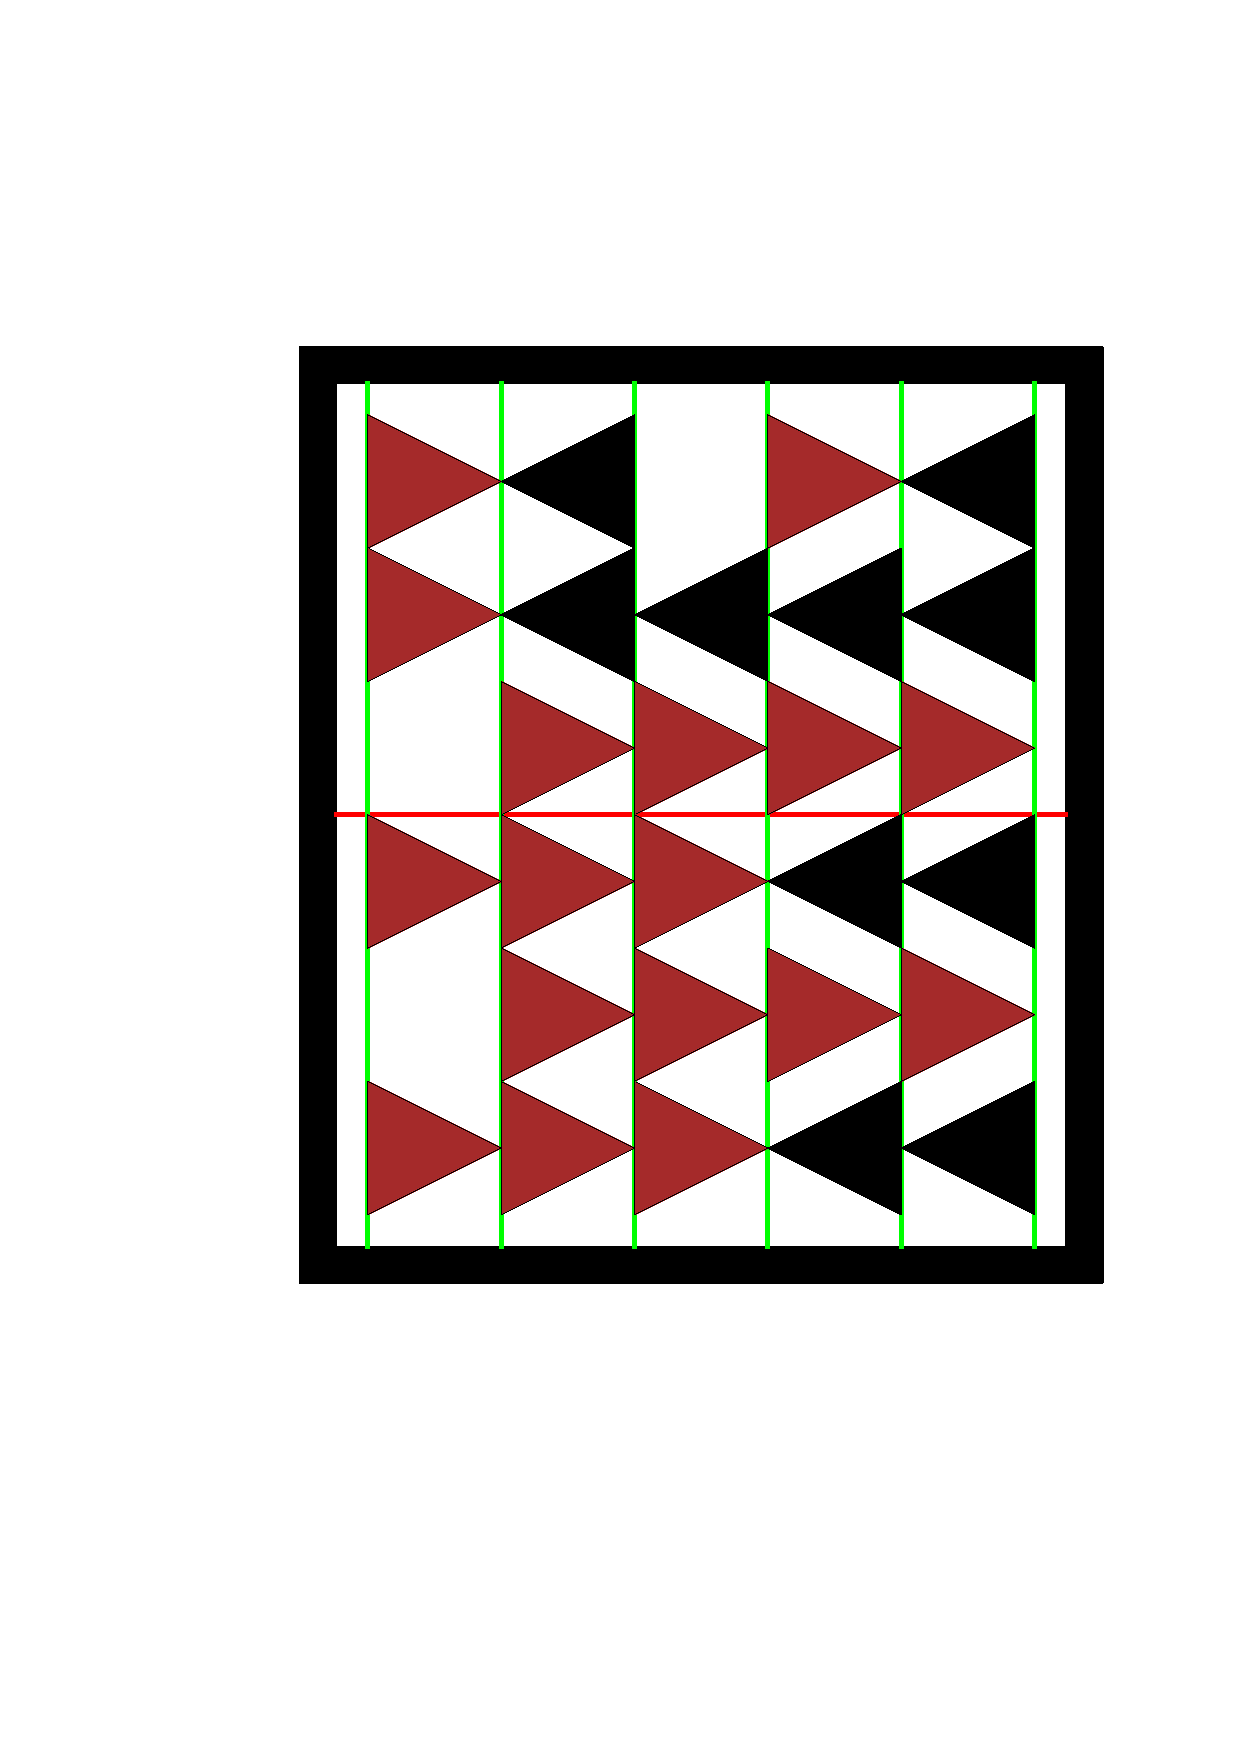
\includegraphics[width=.33\columnwidth]{graphics/LogicEngineFrameFigure5.pdf}
\captionof{figure}{The logic engine from Figure \ref{fig:LogicEngineFrameFigure2Scaled.pdf} whose armatures are rotated}\label{fig:LogicEngineFrameFigure5.pdf}
\end{center}
\end{minipage}

\subsubsection{The Relationship of the Logic Engine and NAE3SAT}

We show that given an Boolean formula in 3-CNF form, $\Phi$, and a truth assignment, $\tau$, where the variables are given a truth assignment such that there is at least one true literal and one false literal in each clause of $\Phi$, then the corresponding logic engine to $\Phi$ is collision-free configurable.
\begin{thm}\label{thm:LogicEngineV3-1}
 Given an instance of a $NAE3SAT$,  it is a ``yes'' instance if and only if the corresponding logic 
engine is collision-free configurable.
\end{thm}
\begin{proof}
Suppose we have an instance of a $NAE3SAT$ that is a ``yes'' instance. This implies that there is a 
truth assignment such that each clause contains a true and a false literal. Now consider the logic 
engine corresponding to this instance. We now 
show that it has a collision free configuration.

For variables that are true, configure the armatures such that the flags corresponding to the 
non-negated literals reside above the 
shaft and the flags that correspond to the negated literals reside below this shaft.  For variables 
that are false, configure the 
armatures in the opposite orientation.  Each clause corresponds to a pair of rows in 
the logic engine, one row for non-negated literals and one for negated literals.  Because the 
$NAE3SAT$ is a yes instance, every row contains at least one unflagged armature.  
By Lemma \ref{lem:logicEngine1}, every row  has a collision-free configuration.

Suppose we have an instance of a $NAE3SAT$ such that the corresponding logic engine has a 
collision-free configuration. By Lemma \ref{lem:logicEngine1} every row at least one unflagged 
armature.  The $k^{th}$ clause is represented by the $k^{th}$ rows above and below the shaft. If the 
literal $x_j$ is found in clause $C_k$, then the armature is unflagged in that row. If the literal 
$\bar{x}_j$ is found in clause $C_k$, then $\bar{l}_{j,k}$ is unflagged.  All flags 
corresponding to negated literals reside below the shaft and flags corresponding to non-negated 
literals reside above the shaft.  All together we have that every clause has a true literal and a 
false literal.  Thus, we have a 'yes' instance of the $NAE3SAT$.
\end{proof}
\begin{thm}\label{thm:LogicEngineV3-2}
Deciding whether a logic engine is collision-free configurable is NP-Hard.
\end{thm}
\begin{proof}
In Table \ref{LogicEngineV3PolynomialTable}, we defined the components of the logic engine in terms of polynomials in $m$ and $n$. 
If there were a polynomial time algorithm that decides whether a given logic engine is collision-free configurable, then by Theorem \ref{thm:LogicEngineV3-1} we would have a polynomial time algorithm to decide whether an instance of the NAE3SAT is a 'yes' instance.  
Since NAE3SAT is NP-Hard \cite{NAE3SATisNPhard}, there is no such algorithm unless $P = NP$.
\end{proof}\section{Logic Engines Represented as Polygonal Linkages}   
In the previous section, we introduced the logic engine.  
This section builds an analogous structure that is formed from a polygonal linkage and we may interchangeably say subcomponent for polygon.
We can modify the mechanical structure of the logic engine to form a polygonal linkage.  
For a given a Boolean formula, $\Phi$, in 3-CNF with $n$ variables and $m$ clauses,
the rigid frame is broken into two polygons, each polygon on the extremity of the structure.
The shaft is broken into $n$ polygons.
Each armature is broken into two parts, each part containing $m$ subcomponents.
In figure \ref{fig:HingedLogicEngineSmall.pdf}, each flag becomes a rectangle.

\begin{minipage}{\linewidth}
\begin{center}
\includegraphics[width=.45\columnwidth]{graphics/HingedLogicEngineSmall.pdf}
\captionof{figure}{A logic engine realized as a polygonal linkage.}\label{fig:HingedLogicEngineSmall.pdf}
\end{center}
\end{minipage}

\subsection{Construction of the Polygonal Linkage Logic Engine}
Suppose we are given an Boolean formula with $m$ clauses and $n$ variables in 3-CNF form, $\Phi$, we construct the polygonal linkage similarly to the logic engine.
The corresponding polygonal linkage $P_\ell = (\PP,\HH)$ is detailed in Table \ref{tbl:hingedPolygonsv3-1a}.

% \begin{minipage}{\linewidth}
\begin{table}
 	\begin{center}
		\begin{tabular}[c]{|l|c|c|c|}
		 \hline
		 Component & Height & Width & Quantity\\ \hline
		 Large Frame Subcomponent & $2\cdot m$ & $1$ & $2$\\ \hline
		 Shaft Subcomponent & $1$ & $3$ & $n$\\ \hline
		 Armature Subcomponent & $2$ & $1$ & $2\cdot m$\\ \hline
		 Flag & $1$ & $1.5$ & $2mn-3m$\\\hline
		\end{tabular}
		\captionof{table}{The components of $\PP$ specified polynomially in terms of the size of the Boolean formula $\Phi$.}\label{tbl:hingedPolygonsv3-1a}
	\end{center}
\end{table}
% \end{minipage}

The large frame subcomponents are hinged on the left most and right most shaft subcomponents. 
Each adjacent shaft subcomponents are hinged and each shaft subcomponent has two orientations, a reflection up and a reflection down about the shaft hinge points.  
On each shaft subcomponent there are two armature shaft subcomponents, one above the shaft subcomponent and one below the shaft subcomponent.  
By the two orientations of the shaft subcomponent, each armature subcomponent has to possible positions.  
Each armature comprises of $m$ armature subcomponents that are hinged together; in total there are $2n$ armatures.  
Each armature subcomponent has two orientations, a reflection left and a reflection right about the armature hinge points.  
Label the armature subcomponents on the $j^\text{th}$ armature starting from the shaft by $\ell_{j,1},\ldots,\ell_{j,n}$ on one side and  $\bar{\ell}_{j,1},\ldots,\bar{\ell}_{j,n}$ on the other side of the shaft.  
Attach a rectangular flag specified in Table \ref{tbl:hingedPolygonsv3-1a}, to some of these segments. 
Each segment is either flagged one or zero flags.
\begin{enumerate}
	 \item If the literal $x_j$ is found in clause $C_k$, then $\ell_{j,k}$ is unflagged.
	 \item If the literal $\bar{x}_j$ is found in clause $C_k$, then $\bar{l}_{j,k}$ is unflagged.
\end{enumerate}

Each flag has two orientations with respect to armature it is attached to.  Each flag has four potential positions, the flag can reflect left or right about the armature and the armature can reflect up or down about the shaft.

\begin{minipage}{\linewidth}
\begin{center}
\includegraphics[width=.33\columnwidth]{graphics/HingedLogicEngineSmallEnumerated.pdf}
\captionof{figure}{A polygonal linkage logic engine that corresponds to the Boolean formula $\Phi = C_1 \cap C_2 \cap C_3$.}\label{fig:HingedLogicEngineSmallEnumerated.pdf}
\end{center}
\end{minipage}

\begin{thm}\label{thm:chp2-HingedPolygons-1}
 Given an instance of a $NAE3SAT$,  it is a ``yes'' instance if and only if the 
corresponding polygonal linkage logic engine has a collision-free configuration.  
\end{thm}
\begin{proof}
Suppose we have an instance of a $NAE3SAT$ that is a ``yes'' instance. This implies that there is a 
truth assignment such that each clause contains a true and a false literal. Now consider the polygonal linkage logic 
engine corresponding to this instance. We now 
show that it has a collision free configuration.

For variables that are true, configure the armatures such that the flags corresponding to the 
non-negated literals reside above the 
shaft and the flags that correspond to the negated literals reside below this shaft.  For variables 
that are false, configure the 
armatures in the opposite orientation.  Each clause corresponds to a pair of rows in 
the polygonal linkage logic engine, one row for non-negated literals and one for negated literals.  Because the 
$NAE3SAT$ is a yes instance, every row contains at least one unflagged armature.  
By Lemma \ref{lem:logicEngine1}, every row  has a collision-free configuration.

Suppose we have an instance of a $NAE3SAT$ such that the corresponding polygonal linkage logic engine has a 
collision-free configuration. By Lemma \ref{lem:logicEngine1} every row at least one unflagged 
armature.  The $k^{th}$ clause is represented by the $k^{th}$ rows above and below the shaft. If the 
literal $x_j$ is found in clause $C_k$, then the armature is unflagged in that row. If the literal 
$\bar{x}_j$ is found in clause $C_k$, then $\bar{l}_{j,k}$ is unflagged.  All flags 
corresponding to negated literals reside below the shaft and flags corresponding to non-negated 
literals reside above the shaft.  All together we have that every clause has a true literal and a 
false literal.  Thus, we have a 'yes' instance of the $NAE3SAT$.
\end{proof}
\chapter{Realizability of Polygonal Linkages with Counter-Clockwise Orientation\label{chapter:polygonalLinkage}} 

We begin the chapter with describing several gadgets that translate the associated graph $A(\Phi)$ of a P3SAT Boolean formula into a hexagonal polygonal linkage.  
These gadgets will be used together to form a special hexagonal linkage that behaves in a similar nature to the logic engine that encoded a NAE3SAT instance of Chapter \ref{chapter:logicEngine} but instead encodes a Planar 3-SAT and its associated graph.  
Given an instance $\Phi$ of P3SAT with $n$ variables and $m$ clauses and its associated graph $A(\Phi)$, 
Together the gadgets will form what is called the auxiliary construction.
A hexagonal polygonal linkage and several gadgets enclosed in a frame (a frame that is conceptually similar to the frame found in a logic engine) would then be used to prove Theorem \ref{thm:hinge3}: it is strongly NP-hard to decide whether a polygonal linkage whose hinge graph is a \textit{tree} can be realized with fixed orientation.

Our proof is a reduction from P3SAT.
Given an instance $\Phi$ of P3SAT with $n$ variables and $m$ clauses and its associated graph $A(\Phi)$, we construct a simply connected polygonal linkage $(\PP,H)$ of polynomial size in $n$ and $m$, such that $\Phi$ is satisfiable if and only if $(\PP,H)$ admits a realization with fixed orientation. 


We construct a polygonal linkage in two main steps: first, we construct an auxiliary structure where some of the polygons have fixed position in the plane (called \emph{obstacles}), while other polygons are flexible, and each flexible polygon is hinged to an obstacle. 
Second, we modify the auxiliary construction into a polygonal linkage by allowing the obstacles to move freely, and by adding new polygons and hinges as well as an exterior \emph{frame} that holds the obstacle polygons in place.
All polygons in our constructions are regular hexagons or long, skinny rhombi.
In Chapter \ref{chp:disk} we ``simulate'' these shapes with disk arrangements to show related results.

Storer, Tamassia, and Tollis \cite{storer1984minimal,tamassia1987efficient} showed that if $G=(V,E)$ is planar where $\vlr{V}=n$ and $\vlr{E} = m$, it can be embedded into a $\vert V \vert \times \vert V \vert$ integer grid where vertices are grid points and an edge are a sequence of alternating horizontal and vertical line segments and bounding total number of bends in an embedding by a bend polynomial $S(n,m)=2.4 \vert V\vert + 4$.  
Now suppose we're given a 3-CNF Boolean formula, $\Phi$, with $i$ variables and $j$ clauses, the associated graph $A(\Phi)$ has $i+j$ vertices.  
We can then define a \textit{fundamental polynomial} $s(n,m)$ that describes the size of the embedding into the plane, $s(n,m) \times s(n,m)$, gives an upper bound on the total number of bends, and accounts for the translation of the associated graph of a P3SAT into a hexagonal polygonal linkage:
$$s(n,m) = 6\lr{3 (n+m) + 4} = 18 (n+m) + 24$$
Note that a planar bipartite graph has at most $2k-4$ by Euler's theorem where $k>2$.  
The tables below are a glossary of formulas and Maclaurin series that are used throughout this chapter.
It will serve as a useful reference for the reader.

$$
\begin{array}{|rcl|}
\hline
z(n,m)		&=& 4 s(n,m)\\\hline
J_h (n,m) 	&=& 6z(n,m)+1 = 24s(n,m)+1 \\\hline
J_d (n,m) 	&=& 4z(n,m)+1												= 16s(n,m)+1  			\\\hline
N(n,m)		&=& \frac{5t-1}{2}											= \frac{5s^\kappa-1}{2}	\\\hline
t(n,m)		&=& s^\kappa																		\\\hline
H(n,m) 		&=&  (12s+1)  \lr{5s^\kappa -1}  \sqrt{3} + 12s \lr{\sqrt{3}+ \frac{1}{250s^\kappa -50}}				\\\hline
\end{array}
$$


$$
\begin{array}{|rcl|}
\hline
&& x 				\leq \sin^{-1} x \leq x + \frac{x^3}{6} \qquad\qquad 0< x <1 \\\hline
&& x - \frac{x^3}{3}\leq \tan^{-1} x \leq x 				\qquad\qquad 0< x < 1\\\hline
&& \frac{x}{2}\leq x - \frac{x^3}{6}\leq \sin x 	 \leq x 				\qquad\qquad 0< x < 1\\\hline
&& 1 - \frac{x^2}{2}\leq \cos x 	 \leq 1 				\qquad\qquad 0< x < 1\\\hline
&& 1 				\leq \sec x 	 \leq 1 + \frac{x^2}{2} \qquad\qquad 0< x < 1\\\hline
\end{array}
$$
The formula $t(n,m)=s^\kappa$ has an exponent $\kappa$ which is a sufficiently large integer chosen later on so that all conditions in this chapter are satisfied.
The trigonometric functions in the table above each are expressed as either the first term or the first and second term of their Maclaurin Series expansion.

\paragraph{Modifying the Associated Graph of a P3SAT.}

Given an instance of P3SAT Boolean formula $\Phi$ of $n$ variables and $m$ clauses with associated graph $A(\Phi)$, we construct a finite \textit{honeycomb} grid $H_{A \lr{\Phi}}$ of regular hexagons over the plane.
We modify the associated graph $A\lr{\Phi}$ by embedding it into honeycomb integer grid in the following way:

\begin{enumerate}
%variables represent cycles of 2m 
\item \textbf{Variable:} A vertex representing a variable shall encompass a consecutive set of hexagons along a horizontal line in the honeycomb (see Figure \ref{fig:VariablesExample.pdf}).

\begin{minipage}{\linewidth}
\begin{center}
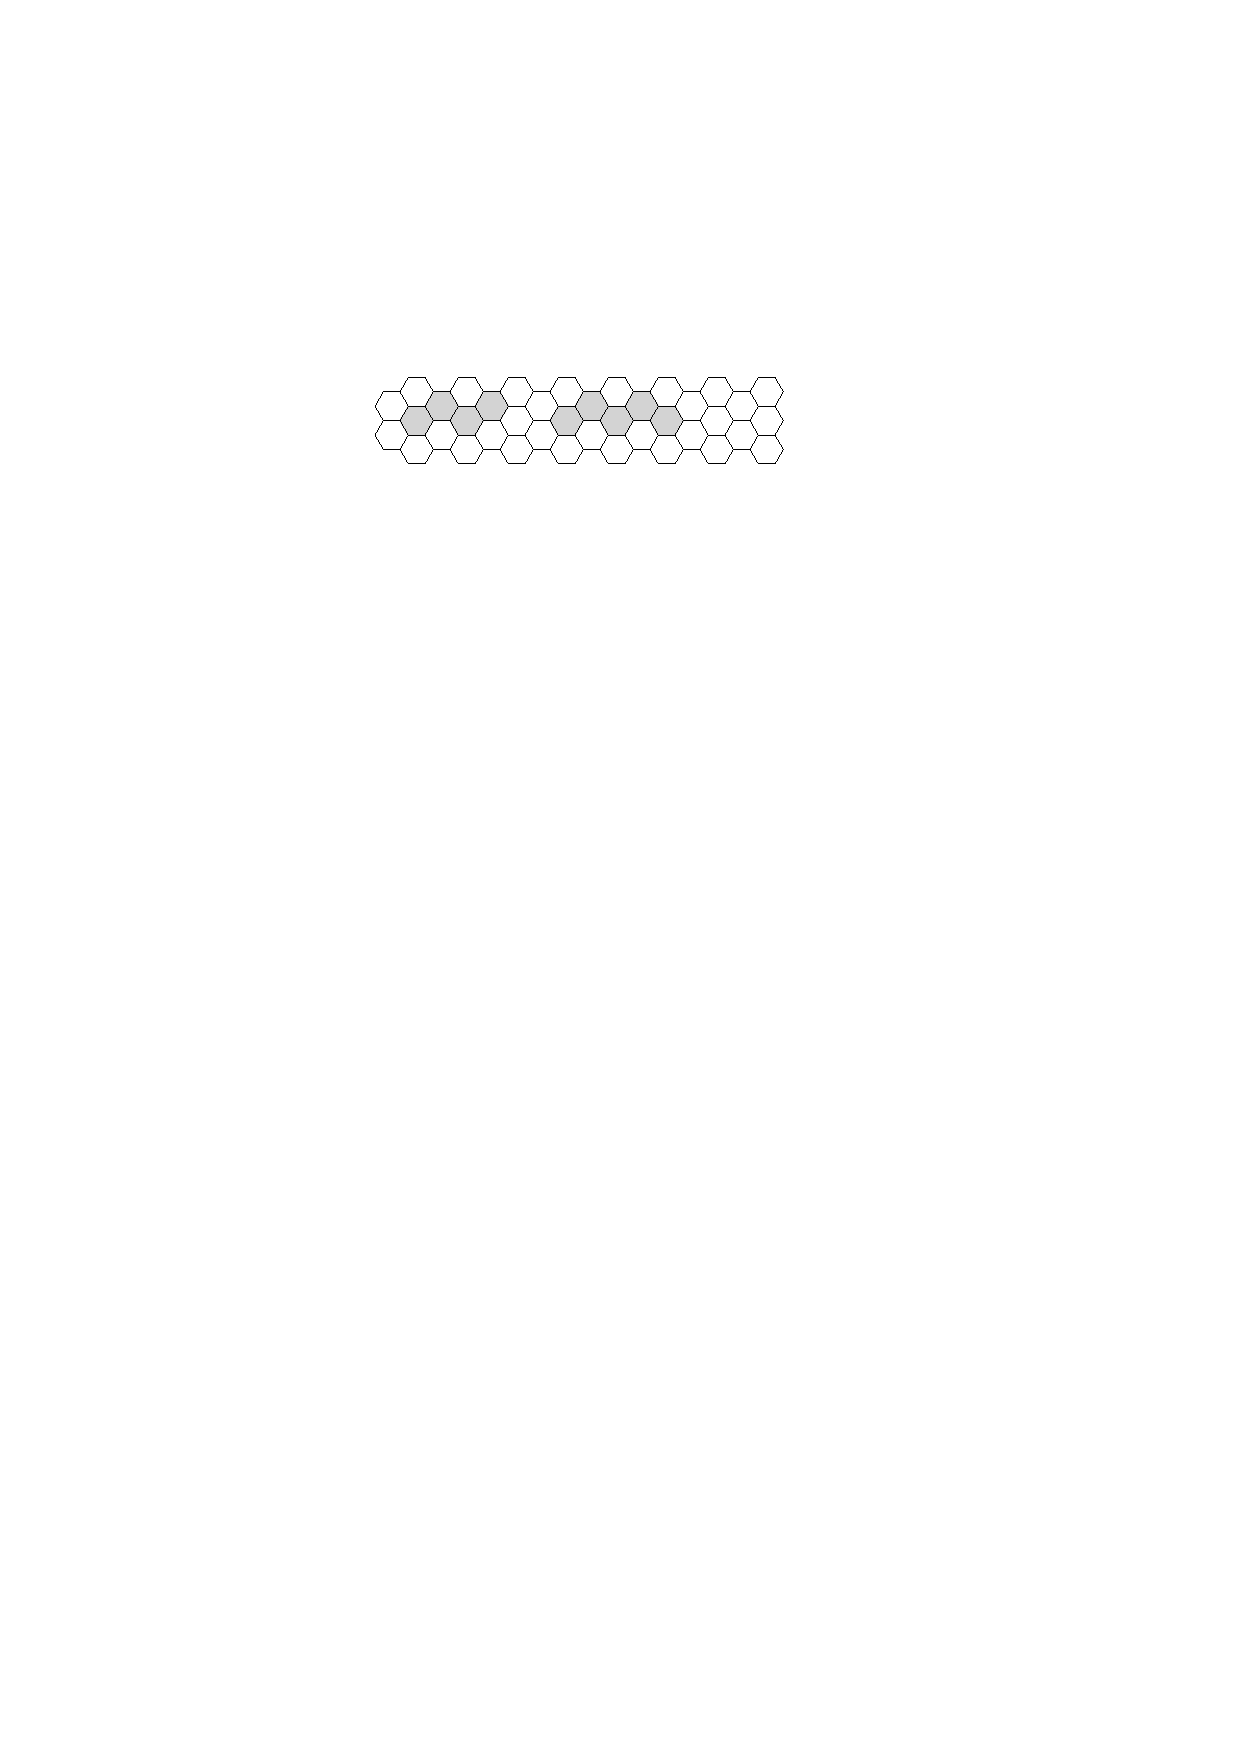
\includegraphics[width=.75\textwidth]{graphics/VariablesExample.pdf}
\captionof{figure}{The four shaded groups of horizontally adjacent hexagons represent four distinct variables from a Boolean formula in the honeycomb.}\label{fig:VariablesExample.pdf}
\end{center}
\end{minipage}

Let $D = \max_{v \in V} \deg(v)$ where $V$ is the set of vertices of $A(\Phi)$.
Every variable vertex $v$  must encompass at least $2 \cdot \deg(v)$ consecutive hexagons but can encompass up to $2 \cdot D$ consecutive hexagons.
\item \textbf{Clause:} A vertex representing a clause shall be a vertex of a hexagon in the honeycomb.
\item \textbf{Edge:} Edges of the associated graph $A(\Phi)$ are paths between the variable $x_i$ and clause $C_j$.  An edge $\left\lbrace x_i, C_j \right\rbrace$ of the associated graph is pairwise edge disjoint. 
The edges of the drawing shall traverse the edges of hexagons in a vertically or horizontally zigzagging manner (see Figure \ref{fig:HoneyCombAssociatedGraphSmall}) in the honeycomb from the literal to the corresponding clause. 
Edges traverse a hexagon in two edges vertically, three edges horizontally.  
The vertical zigzagging edge segments traverse the left or right sides of a hexagon(s).
The horizontal zigzagging edge segments traverse the top or bottom halves of a hexagon(s).
When the edge transitions from a vertical to horizontal traversal, the edge traverses in over 4 edges about the hexagon.
The length of the edges are bounded above by $6 \cdot \lr{\ell_1 \lr{x_i,C_j} + D}$ where $\ell_1$ is the $L_1$ norm and $x_i$ and $C_j$ are points in the grid plane. 
\end{enumerate}

\begin{minipage}{\linewidth}
\begin{center}
\includegraphics[width=.9\textwidth]{graphics/HoneyCombAssociatedGraphSideBySide.pdf}
\captionof{figure}{
(a) This is an instance of an associated graph for a P3SAT overlayed onto a honeycomb grid and placed into a regular hexagonal region.
This honeycomb graph could correspond to Boolean formula $\lr{\lnot x_1 \lor \lnot x_2 \lor x_4} \land \lr{x_2 \lor \lnot x_3 \lor x_4} \land \lr{x_1 \lor \lnot x_3 \lor \lnot x_4}$. (b) This is the same instance as (a) shown without the hexagonal region.
}\label{fig:HoneyCombAssociatedGraphSmall}
\end{center}
\end{minipage}

Figure \ref{fig:HoneyCombAssociatedGraphSmall} illustrates an associated graph of a P3SAT overlayed on a honeycomb.
Let the region in which the construction lies in be a regular hexagon region with polynomial side length $s(n,m)$. 
The honeycomb construction will act as preliminary concept that will be refined further in the Auxiliary Construction.\section{Auxiliary Construction}\label{sec:auxiliaryConstruction}
Let $\Phi$ be a Boolean formula of P3SAT with variables $x_1,\ldots , x_n$ and clauses $C_1,\ldots ,C_m$, where $A(\Phi)$ is the associated planar graph and $\tilde{A}\lr{\Phi}$ be corresponding honeycomb graph.
We continue to modify $\tilde{A}\lr{\Phi}$ to form the auxiliary construction.   
Consider a large (polynomial-size) regular hexagon $J$  with side length $s(n,m)$ that contains all gadgets in our construction and hexagonal grid.
For each hexagon of the hexagonal grid contained in $J$, scale the hexagon in the following way: first we fix the center of the hexagon and then scale (shrink) the hexagon; adjacent hexagons in the honeycomb no longer touch each other and form corridors and junctions between the hexagons (See Figure \ref{fig:ScalingForCorridors.pdf}). 

\begin{minipage}{\linewidth}
\begin{center}
\includegraphics[width=.4\columnwidth]{graphics/ScalingForCorridors.pdf}
\captionof{figure}{(a) This figure shows a region of a hexagonal grid scaled in place to form corridors between adjacent hexagons(shown in (b)).}\label{fig:ScalingForCorridors.pdf}
\end{center}
\end{minipage}

Formally, let a \textit{corridor} be a channel between two adjacent hexagons and a \textit{junction} be a region where three corridors meet.

\textbf{Formal Description of the Auxiliary Construction.}
Given the side length of $J$, $s(n,m)$, we need to scale the grid of hexagons of the hexagonal grid in the interior of $J$ accordingly.

\begin{minipage}{\linewidth}
\begin{center}
\includegraphics[width=.9\columnwidth]{graphics/hexagonalConstructionOfJSmallWithoutHalfHexagons.pdf}
\captionof{figure}{(a) shows a \textit{formal auxiliary construction} with $k=2$. $k$ is the number of hexagons of the hexagonal grid in the interior of $J$ that is on the bottom most row.  (b) shows a formal auxiliary construction with $k=3$. (c) shows a formal auxiliary construction with $k=4$.  Note that in each figure}\label{fig:hexagonalConstructionOfJSmallWithoutHalfHexagons.pdf}
\end{center}
\end{minipage}

In Figure \ref{fig:hexagonalConstructionOfJSmallWithoutHalfHexagons.pdf}, we show the three smallest possible formal constructions of $J$, $J_1, J_2, J_3$.  
A formal construction of $J$ is when six hexagons of the hexagonal grid each have two adjacent sides lie on the perimeter of $J$.
We have shown informal construction earlier where this does not occur.
Unless otherwise specified, we will assume the use formal constructions.
Each of the figures in Figure \ref{fig:hexagonalConstructionOfJSmallWithoutHalfHexagons.pdf} shows $J$ in bold and the hexagonal grid in its interior.
Notice that in each case we have six hexagons of the hexagonal grid with each of the six hexagons having two adjacent sides that lie on the perimeter of $J$.

The height and diameter of $J$ can be described in terms of hexagons in the grid a vertical or horizontal line may cross. 
We'll denote these qualities as the hexagonal height and hexagonal diameter of $J$.  
Figures \ref{fig:hexagonalConstructionOfJSmallWithoutHalfHexagons.pdf}(c) and \ref{fig:hexagonalConstructionOfJSmallWithoutHalfHexagons.pdf}(a) show the hexagons of the hexagonal height and hexagonal diameters of $J_1$ and $J_3$ respectively.  
The formula for calculating hexagonal height of $J_z$ is 
\begin{equation}\label{eqn:Jh}
J_h (n,m) = 6z(n,m)+1
\end{equation}
The formula for calculating the hexagonal diameter of $J_z$ is 
\begin{equation}\label{eqn:Jd}
J_d (n,m) = 4z(n,m)+1
\end{equation}
Since the associated graph of a P3SAT instance can be encoded into a honeycomb grid of size $s(n,m) \times s(n,m)$, then let $z(n,m)=4\cdot s(n,m)$ to enclose the same honeycomb to be enclosed into the interior of $J_z$.

\begin{minipage}{\linewidth}
\begin{center}
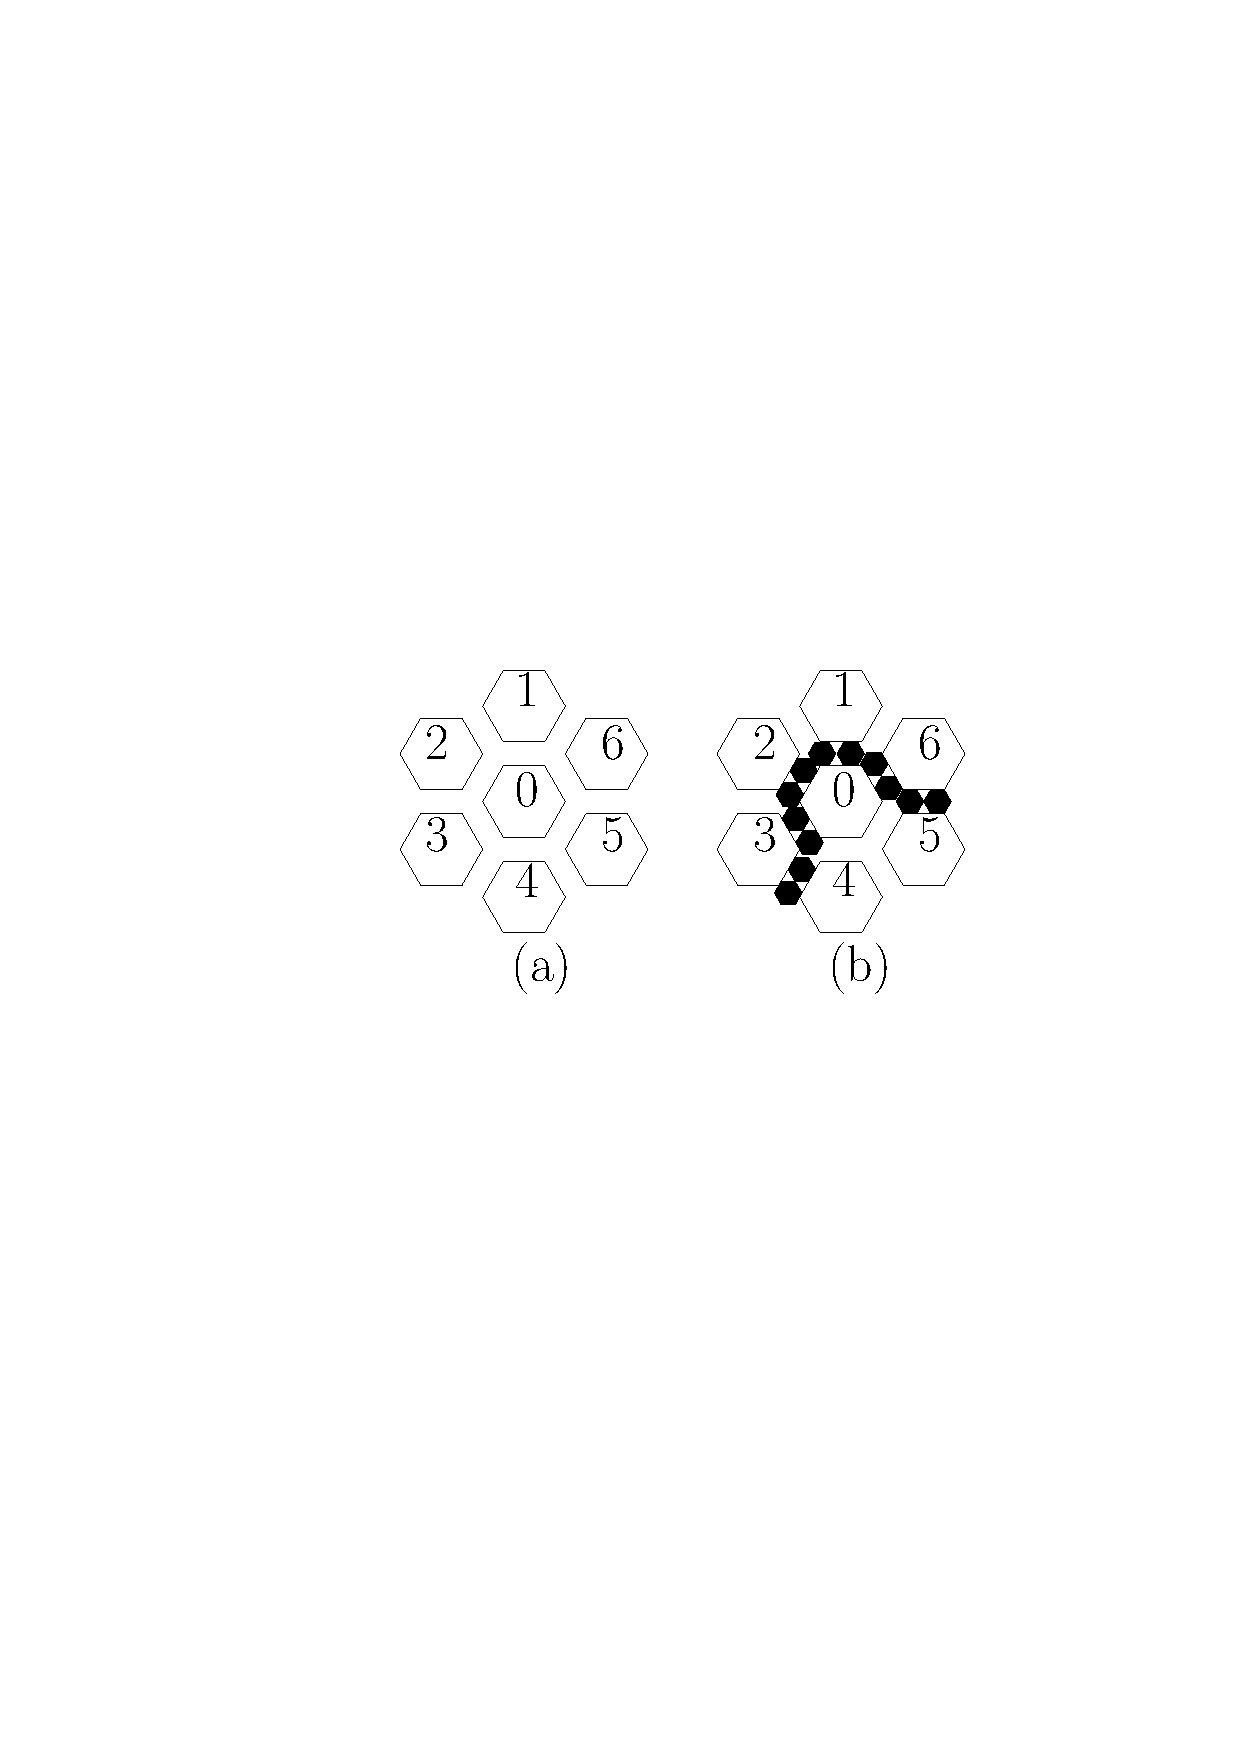
\includegraphics[scale=.66]{graphics/FlexibleHexagons.pdf}
\captionof{figure}{
(a) A region of the honeycomb shown with scaling. The corridors and junctions formed from the first scaling is preserved after scaling the honeycomb grid to where the side lengths of the hexagon are $N(n,m)$.
(b) The same region in (a) containing flags.
}\label{fig:HoneycombFlixible.pdf}
\end{center}
\end{minipage}



The obstacle hex Figure \ref{fig:HoneycombFlixible.pdf}(a) be obstacle hexagons that are fixed.
In Figure \ref{fig:HoneycombFlixible.pdf}(b), we have smaller hexagons within some corridors and junctions.
These hexagons are flags.
For each edge in $\tilde{A}(\Phi)$, we insert flags into the corridor corresponding to that edge.
%Flags are hinged at the vertex closest to origin and the side of the corridor (See Figure \ref{fig:variable}).
Flags are regular hexagons that reside in the corridors and junctions; each flag is hinged to a obstacle hexagon (see Figure \ref{fig:HoneycombFlixible.pdf}(b)).  
For any of these corridors, we attach hinges to the boundary of the corridor; pick an arbitrary side for all hinges.  
The first and last hinge are one unit from the obstacle hexagon corners, the hinges between the first and last hinge are 2.5 units apart.  
Let $t(n,m)=s^\kappa$ be the number of flags in a corridor (see Figure \ref{fig:variable}). 
Scale $J$ and the obstacle hexagons in the interior of $J$ independently from their centers (see Figure \ref{fig:ScalingForCorridors.pdf}) such that each obstacle hexagon has side length: $$N(n,m)=\frac{5t(n,m)-1}{2}.$$ 

\begin{minipage}{\linewidth}
\begin{center}
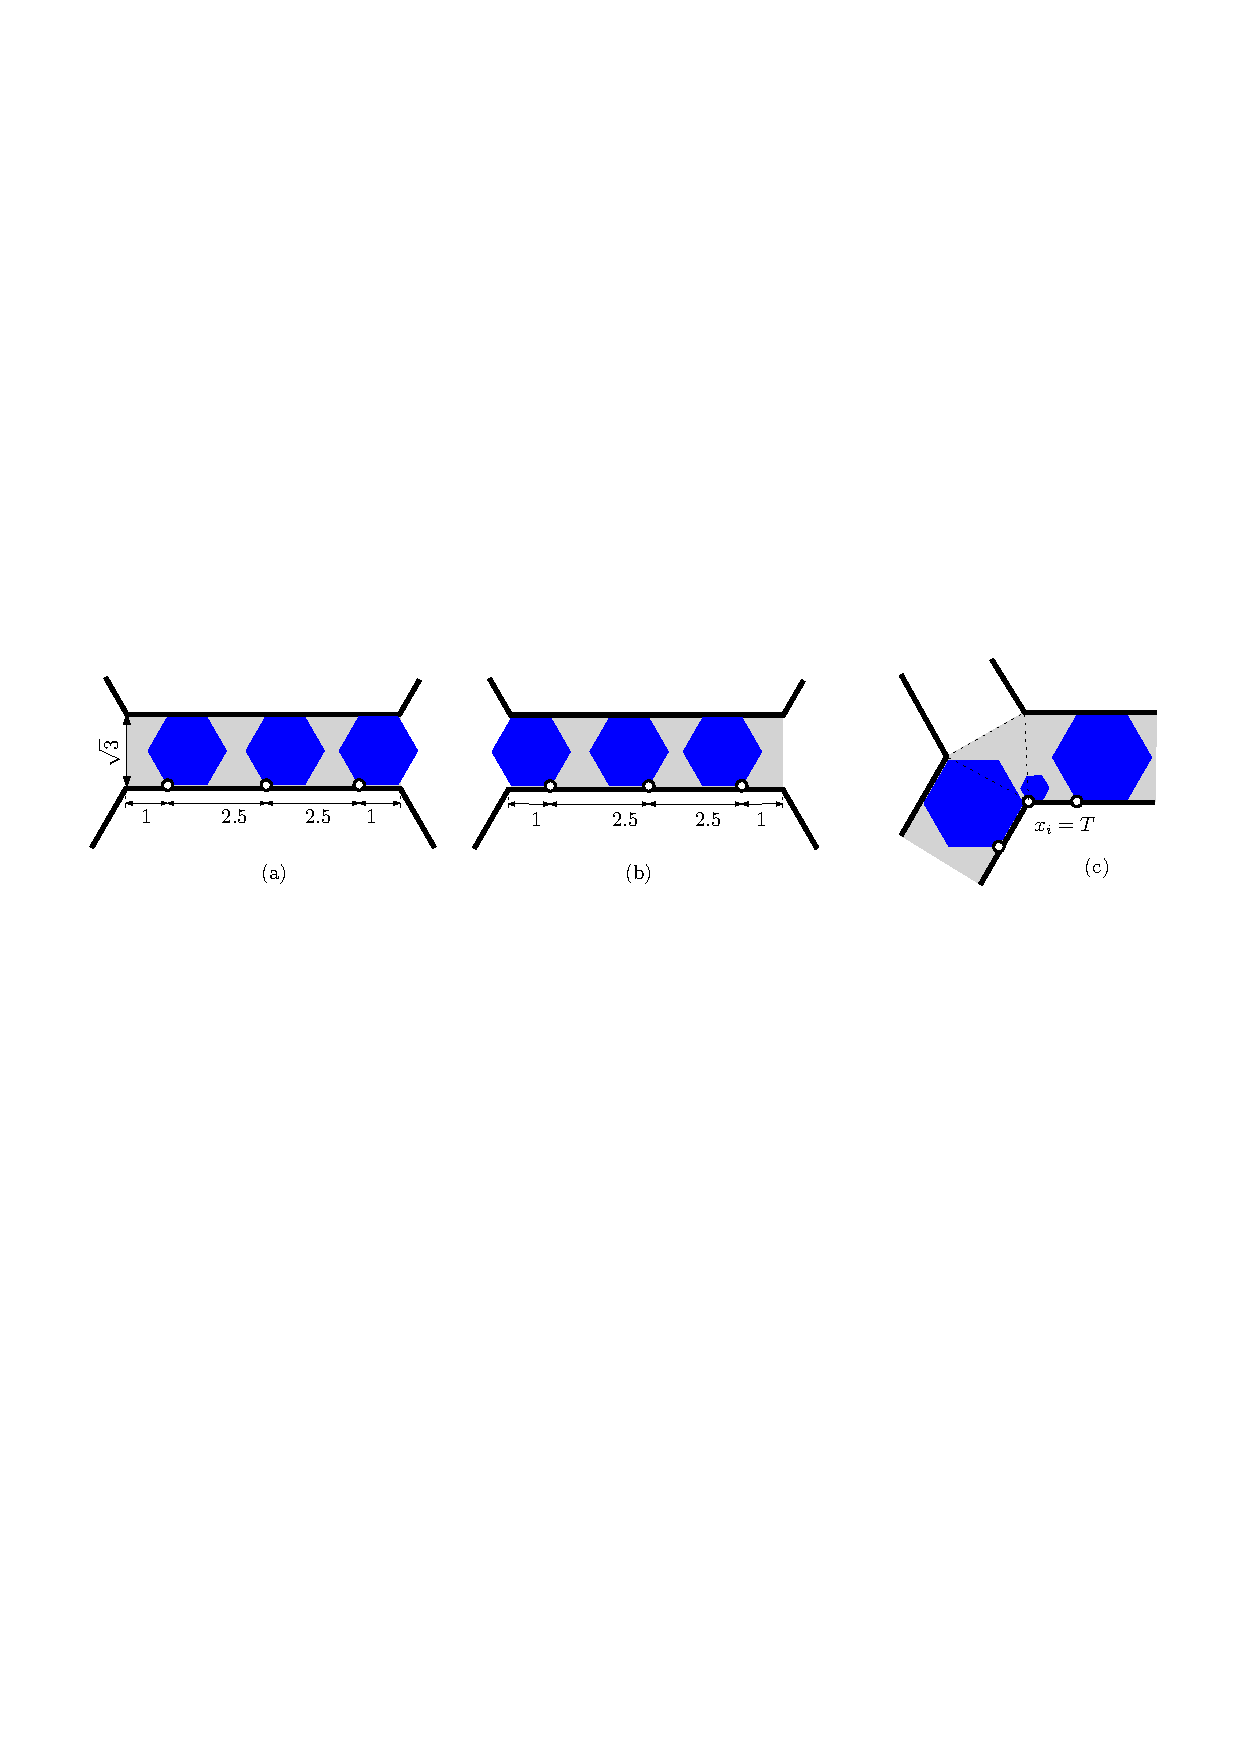
\includegraphics[width=0.9\columnwidth]{graphics/fig-variable-hex+}
\captionof{figure}{
(a) A corridor when all unit hexagons are in state R.
(b) A corridor where all unit hexagons are in state L.
(c) A junction where a small hexagon between two corridors
    ensures that at most one unit hexagon enters the junction from those corridors.}\label{fig:variable}
\end{center}
\end{minipage}

Between two adjacent obstacle hexagons, there is a $\frac{5t-1}{2}\times \sqrt{3}$ rectangular corridor.  %, which we call corridor. 
Three adjacent corridors meet at a regular triangle, which we call a junction. 

We next describe variable, clause, and transmitter gadgets.
The basic building block of both variable and transmitter gadgets consists of $t$ regular hexagons of side length 1 (\emph{unit hexagons}, for short) attached to a wall of a corridor such that the hinges divide the wall into $t+1$ intervals of length $(1,2.5,\ldots ,2.5,1)$ as shown in Fig.~\ref{fig:variable}(a-b). 

\paragraph{Variable Gadget.}
The {\bf variable gadget} for variable $x_i$ is constructed as follows. 
Recall that variable $x_i$ corresponds to a cycle in the associated graph $\tilde{A}(\Phi)$, which has been embedded as a cycle in the hexagonal tiling, with corridors and junctions. 
In each junction along this cycle, attach a small hexagon in the common boundary of the two corridors in the cycle. 
Figure \ref{fig:VariableGadgetSmall.pdf} depicts a \textit{variable gadget} in the hexagonal grid.

\begin{minipage}{\linewidth}
\begin{center}
\includegraphics[width=0.45\columnwidth]{graphics/VariableGadgetSmall.pdf}
\captionof{figure}{This depicts a variable gadget with $x_1 = T$.  Carefully note that the flags around $x_1$ are in the state $R$. Corridors adjacent to two obstacles of a variable in the honeycomb do not have $t$ flags; these corridors simply have the flags at the junctions.}\label{fig:VariableGadgetSmall.pdf}
\end{center}
\end{minipage}

For each junction in the transmitter gadget, we attach a small hexagon in the junction as shown in Figure \ref{fig:transmitter} except at the clause junction.
 A {\bf transmitter gadget} is constructed for each edge $\left\lbrace x_i,C_j\right\rbrace$ of the graph $A(\Phi)$; it consists of a sequence of junctions and corridors from a variable gadget's junction to a clause junction.  
Choosing the location of the small hexagon depends on whether the non-negated or negated literal is found in the clause.
\begin{itemize}
\item[(a)]  For an edge $(x_i,C_j)$ of the graph $A(\Phi)$, if the non-negated literal of $x_i$ exists in $C_j$, attach the small hexagon to the left side of the junction (see Figure \ref{fig:VariableJunctionTransmitterSelection.pdf}(a)).
\item[(b)]  For an edge $(x_i,C_j)$ of the graph $A(\Phi)$, if the negated literal of $x_i$ exists in $C_j$, attach the small hexagon to the right side of the junction (see Figure \ref{fig:VariableJunctionTransmitterSelection.pdf}(b)).
\end{itemize}
\paragraph{Clause Gadget.}
Recall that a clause from a Boolean formula $\Phi$ in 3-CNF has three literals.  If $\Phi$ is a  'yes' instance, then at least one literal in every clause of $\Phi$ is true.  We construct the clause gadget to model this fact about Boolean formulas in 3-CNF.

The {\bf clause gadget} lies at a junction adjacent to three transmitter gadgets (see Fig.~\ref{fig:clause} and Section \ref{transmitterGadget}). 
At such a junction, we attach a unit line segment to an arbitrary vertex of the junction, and a small hexagon of side length $\frac{1}{3}$ to the other end of the segment. 
If unit hexagons enter the junction from all three corridors (i.e., all three literals are false), then there is no space left for the small hexagon (see Lemma \ref{lem:aux-1}).

\begin{minipage}{\linewidth}
\begin{center}
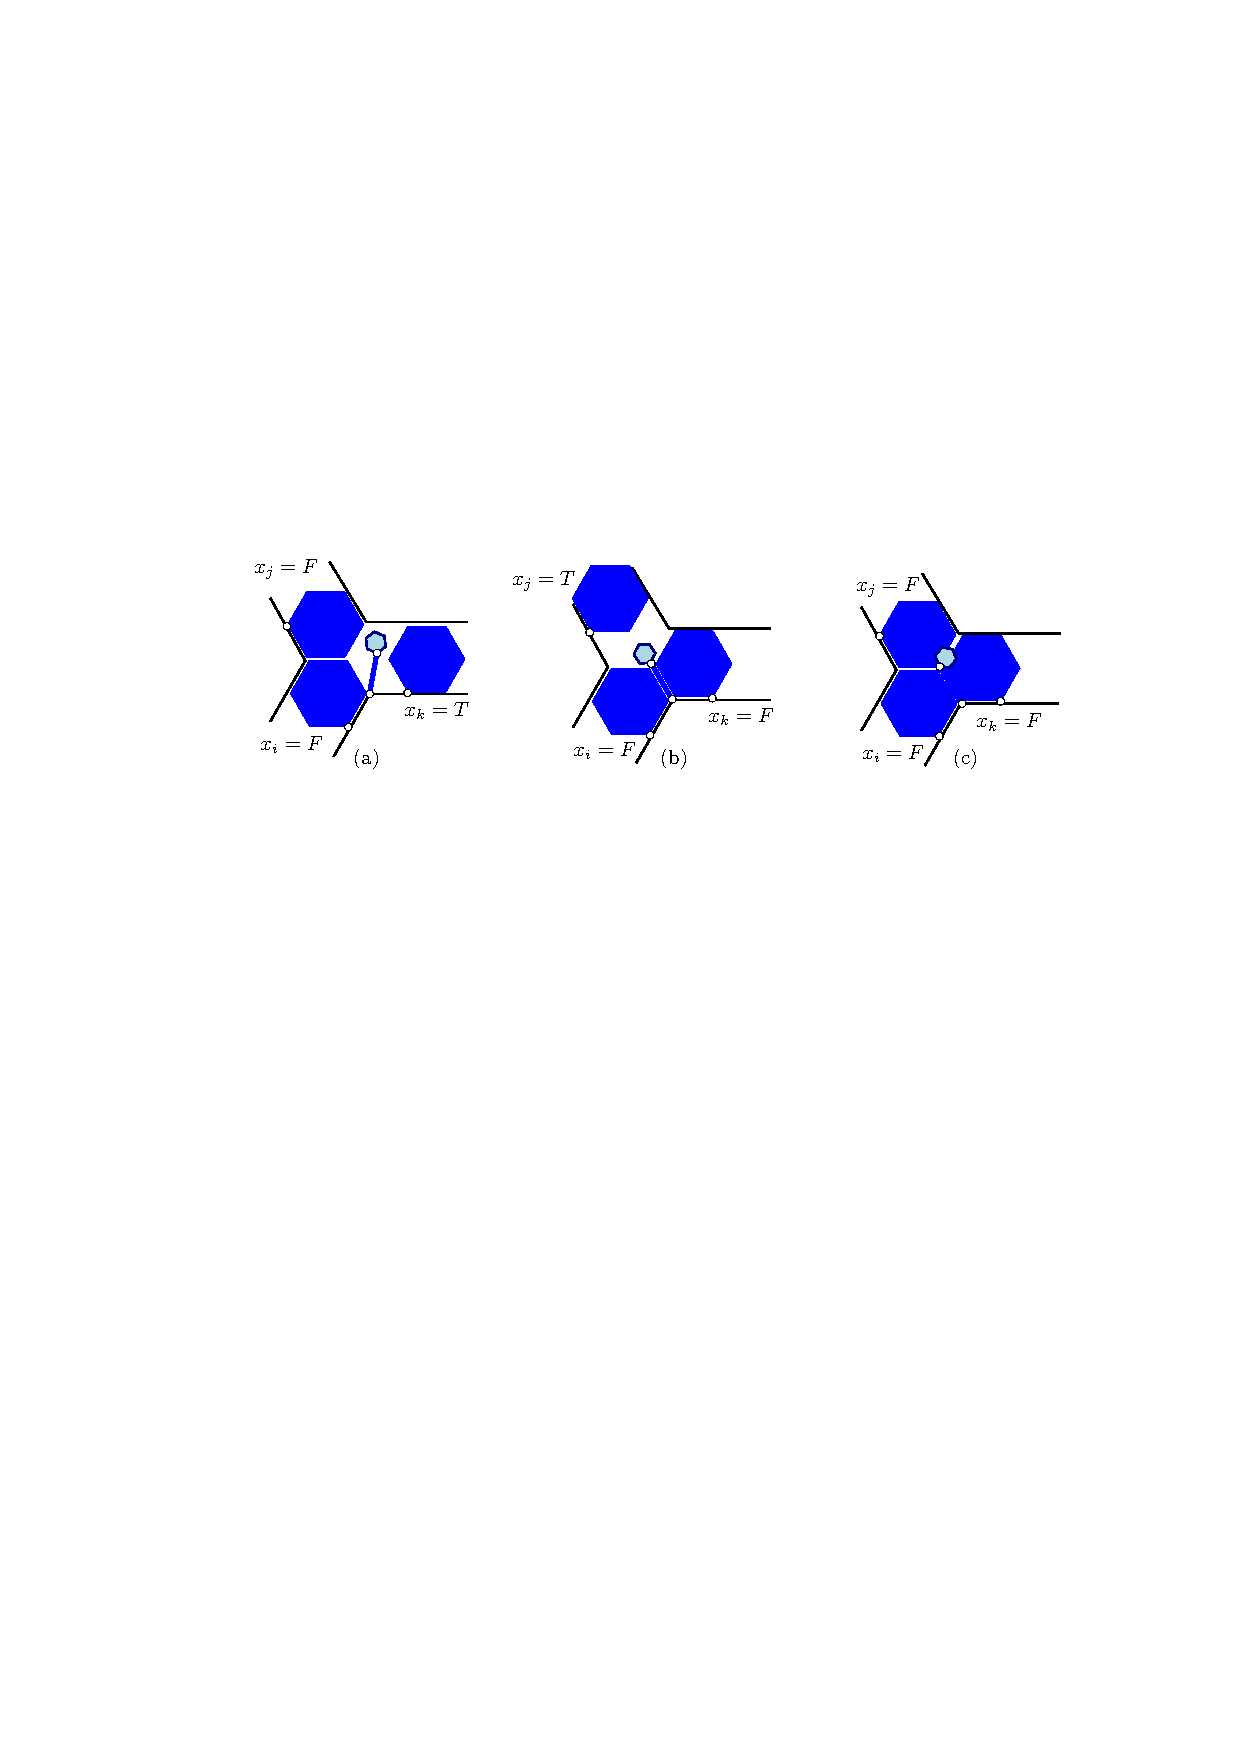
\includegraphics[width=0.7\columnwidth]{graphics/fig-clause-hex}
\captionof{figure}{(a-b) A clause gadget $(x_i\vee x_j\vee x_k)$ is
    realizable when at least one of the literals is {\sc True}.
    (c) The clause gadget cannot be realized when all three literals are {\sc False}.}\label{fig:clause}
\end{center}
\end{minipage}

\paragraph{Transmitter Gadget.\newline }\label{transmitterGadget}

\begin{minipage}{\linewidth}
\begin{center}
\includegraphics[width=0.7\columnwidth]{graphics/fig-assoc-hex}
\captionof{figure}{Left: the associated graph $A(\Phi)$ for a Boolean formula $\Phi$.
Right: the schematic layout of the variable, clause, and transmitter gadgets in the auxiliary construction showing in Section \ref{sec:auxiliaryConstruction}}\label{fig:assoc2}
\end{center}
\end{minipage}

In the associated planar 3-SAT graph $A(\Phi)$, every variable vertex has an cyclic order of edges.
Suppose we have a variable vertex $x_i$ with counter-clockwise cyclic order of edges $\left(\left\lbrace x_i,C_1\right\rbrace\right.$, $\left\lbrace x_i,C_2\right\rbrace$, $\ldots$, $\left.\left\lbrace x_i,C_k\right\rbrace\right) $.  
Assign distinct junctions of the variable cycle of $x_i$ to the edges $\left\lbrace x_i,C_j\right\rbrace$ in the same cyclic order (refer to Figure \ref{fig:assoc2} for an example).

\begin{minipage}{\linewidth}
\begin{center}
\includegraphics[width=0.80\columnwidth]{graphics/VariableJunctionTransmitterSelection2.pdf}
\captionof{figure}{These two figures depict an example of placing a transmitter gadget corresponding to edge $\left\lbrace x_i, C_j \right\rbrace$.}
\label{fig:VariableJunctionTransmitterSelection.pdf}
\end{center}
\end{minipage} 

Figure \ref{fig:VariableJunctionTransmitterSelection.pdf} shows an example of each rule on choosing a junction to attach a transmitter gadget.
In this figure, both variable gadgets are in state $R$, i.e. variable $x_i = T$.  
Figure \ref{fig:VariableJunctionTransmitterSelection.pdf}(a) we have a transmission of ``true'' between the variable and clause gadget.

\begin{minipage}{\linewidth}
\begin{center}
	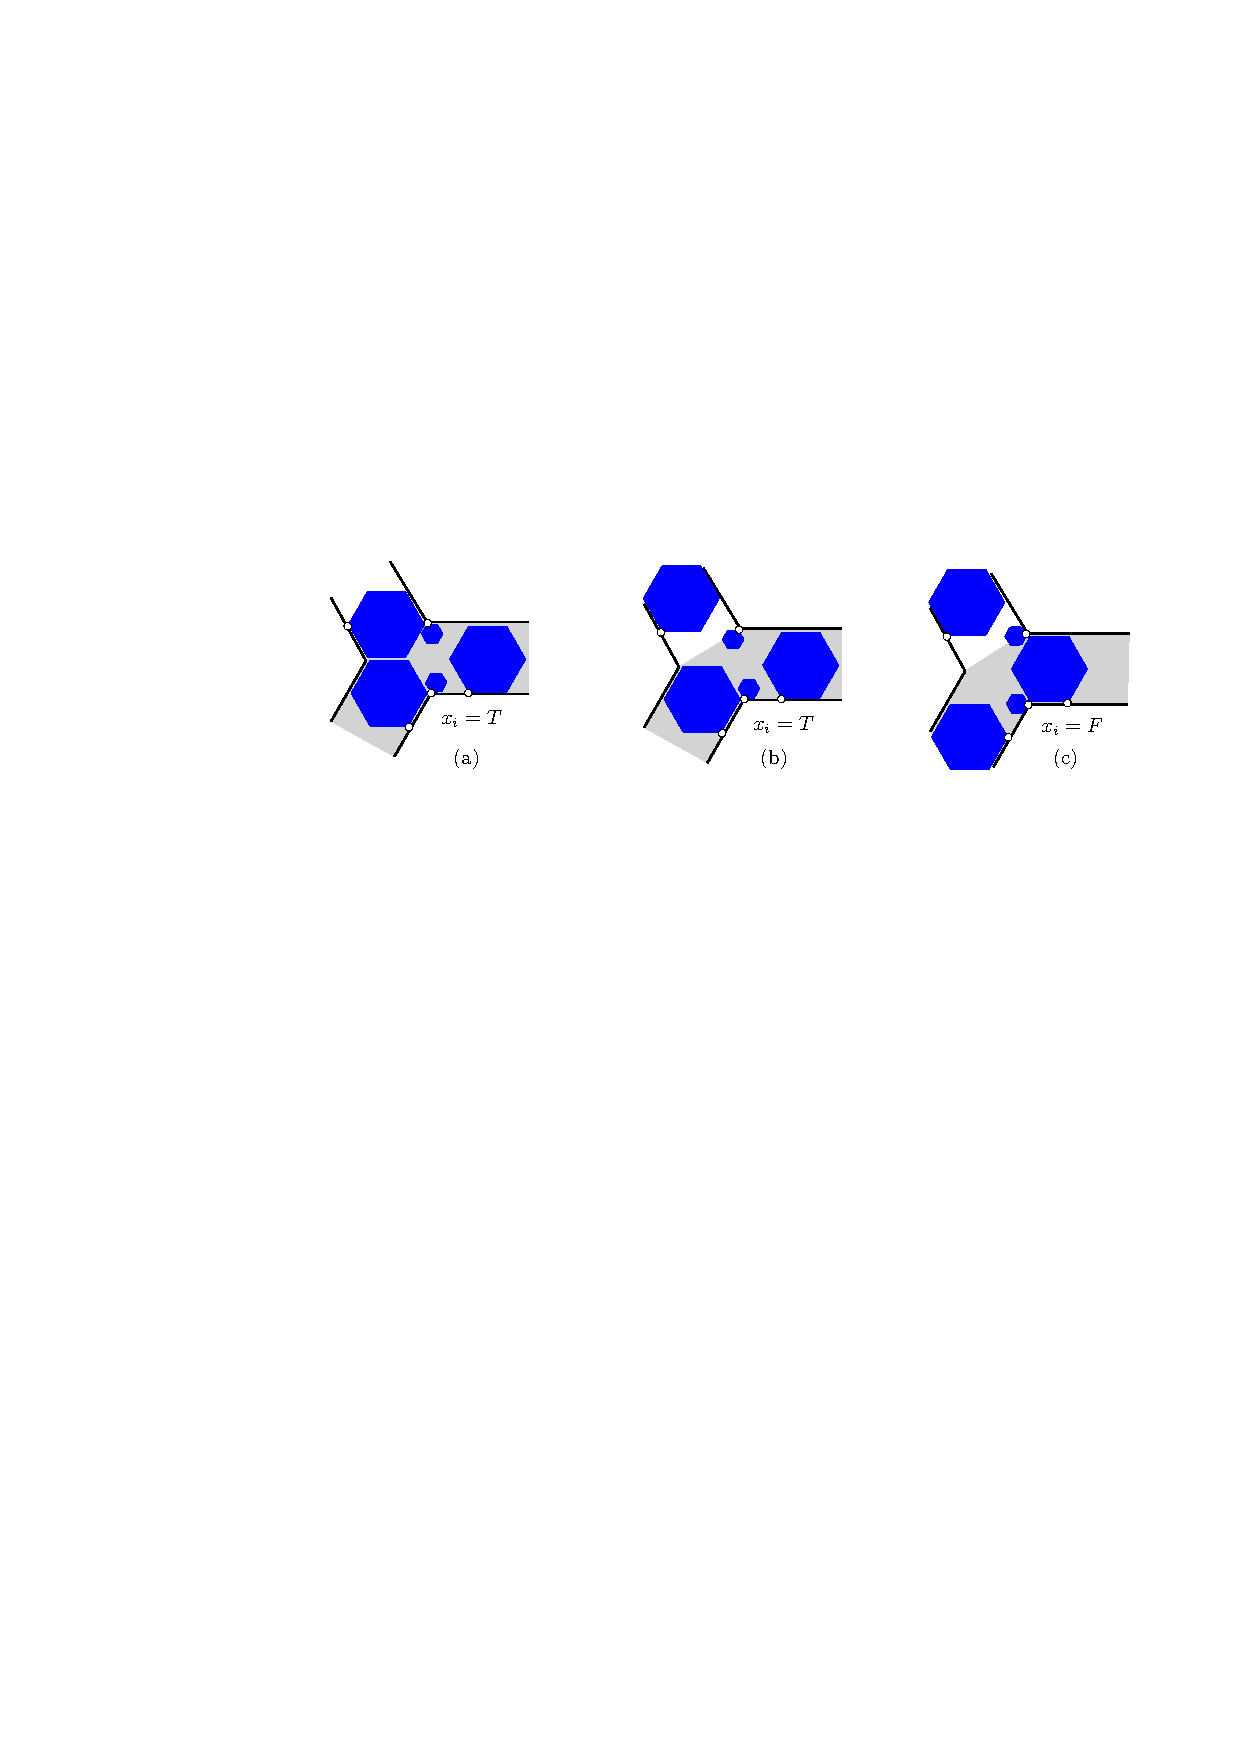
\includegraphics[width=0.7\columnwidth]{graphics/fig-transmitter-hex}
	\captionof{figure}{The common junction of a variable gadget and a transmitter gadget.
(a) When $x_i=T$, a hexagon of the transmitter may enter the junction of the variable gadget.
(b) When $x_i=T$, the transmitter gadget has several possible realizations.
(c) When $x_i=F$, no hexagon from the transmitter enters a junction of the variable gadget.}
	\label{fig:transmitter}
\end{center}
\end{minipage} 

This completes the description of the auxiliary construction.

\section{Functionality of the Auxiliary Construction and Gadgets}

For each corridor, there are two junctions adjacent to it; of these two junctions, we denote the junction from which a flag in the corridor enters into as the \textit{active junction} (see Figure \ref{fig:ActiveChannel.pdf}).  

\begin{minipage}{\linewidth}
\begin{center}
\includegraphics[width=0.9\columnwidth]{graphics/ActiveChannel.pdf}
\captionof{figure}{The active junction in (a) is the junction on the left and in (b) the active junction is on the right.  The active junction is the junction in which a flag enters from a corridor.}\label{fig:ActiveChannel.pdf}
\end{center}
\end{minipage}

Section \ref{sec:auxiliaryConstruction} is a formal description of the auxiliary construction and its gadgets.
This subsection covers the underlying assumptions and proofs about the functionality of the auxiliary construction.
Throughout this section we assume that the polygonal linkage is realizable, i.e. no two polygons overlap.  
The first observations about the functionality of the auxiliary construction are about the flags.  
For $t$ flags in a corridor, the following holds:
\begin{observation}\label{obs:corridor}

\begin{itemize}

\item[(1)] If the leftmost flag is in state R, then all $t$ flags are in state R, and the rightmost flag enters the junction on the right of the corridor.
\item[(2)] Similarly, if the rightmost flag is in state L, then all $t$ flags are in state L, and the leftmost flag enters the junction on the left of the corridor.
\end{itemize}
\end{observation}

Observation~\ref{obs:corridor} and the small hexagons ensure that the state of any flag along the cycle determines the state of all other unit hexagons in the cycle. 
This property defines the binary variable $x_i$: if all flags in the top horizontal corridors are in state R and $x_i=F$, then $x_i=T$ and all hexagons are all in state L.

When a binary variable $x_i = T$, we will say that the variable in state $R$ and that the cycle of small hexagons around the variable gadget are in a ``clockwise direction''.
When a binary variable $x_i = F$, we will say that the variable is in state $L$ and that the cycle of small hexagons around the variable gadget are in a ``counter-clockwise direction''. 

The proof of the Observation \ref{obs:corridor} is similar to the proof of Lemma \ref{lem:logicEngine1} regarding a row in a logic engine having a collision-free configuration.
\begin{proof}
Suppose the leftmost hexagon, $h_1$, is in state $R$ in a corridor.
Denote the $t$ flags in a corridor as $h_1$, $h_2$, $\ldots$, $h_t$ from leftmost to rightmost respectively.
$h_2$ must be in state $R$ otherwise we result in a collision between $h_1$ and $h_2$.
Without loss of generality, $h_i$ and $h_{i+1}$ must be in a state $R$ in order to prevent an adjacent flag collision. 
This implies that rightmost flag $h_t$ must also be in state $R$; this implies that $h_t$ enters the junction that is on the right of the corridor.

Similarly, suppose the rightmost hexagon, $h_t$, is in state $L$ in a corridor.
Denote the $t$ flags in a corridor as $h_1$, $h_2$, $\ldots$, $h_t$ from leftmost to rightmost respectively.
$h_{t-1}$ must be in state $L$ otherwise we result in a collision between $h_t$ and $h_{t-1}$.
Without loss's of generality, $h_i$ and $h_{i+1}$ must be in a state $L$ in order to prevent an adjacent flag collision. 
This implies that rightmost flag $h_1$ must also be in state $L$; this implies that $h_1$ enters the junction that is on the left of the corridor.
\end{proof}

\begin{observation}\label{obs:junction}
If a small hexagon is attached to a vertex at a junction between two adjacent corridors, then a flag can enter the junction from at most one of those corridors.
\end{observation}
\begin{proof}
Suppose there is a small hexagon attached to a vertex at a junction between two adjacent corridors.
Suppose it is not that case that a flag can enter the junction from at most one of these adjacent corridors.
Then there are two flags entering the junction, one from each adjacent corridor.
The angular sum of the vertex about the adjacent corridors consists of the obstacle hexagon, both flags, and the small unit hexagon.
Each angle of each hexagon is $\frac{2 \pi}{3}$ radians, totalling to an angular sum of $\frac{8 \pi}{3} > 2 \pi$.
This is a contradiction with the total angular sum of a vertex on the plane to be $2 \pi$.
\end{proof}

The flags of the auxiliary construction help communicate the Boolean value of a variable gadget to the rest of the auxiliary construction.
This property of the flags in a corridor is analogous to the flags in a row of a logic engine.

Observations \ref{obs:corridor} and \ref{obs:junction} ensure that the state of any unit hexagon along the cycle determines the state of all other unit hexagons in the cycle. 
This property defines the binary variable $x_i$: If $x_i=T$, then all unit hexagons in the top horizontal corridors are in state R; and if $x_i=F$, they are all in state L.

For a variable gadget $x_i$, we distinguish the upper half and lower half of the gadget in the variable cycle.
Then we have the following lemma:
\begin{lem}\label{lem:aux-2}
If variable $x_i = T$, then all flags in the upper half of the variable gadget are in state $R$ and all flags in the lower half of the variable are in state $L$; if variable $x_i = L$, then all flags in the upper half of the variable gadget are in state $L$ and all flags in the lower half of the variable gadget are in state $R$.    
\end{lem}
This lemma serves to show that the truth or falsity of a variable is consistent throughout the gadget.
\begin{proof}
Suppose we have two adjacent corridors $k_i$ and $k_{i+1}$ sharing junction $J_i$ and without loss of generality, $k_i$ is the left most corridor.
Observation \ref{obs:junction} implies that there can only be one hexagon entering $J_i$ from either $k_i$ or $k_{i+1}$. If the hexagon that enters $J_i$ is from corridor $k_i$, then this hexagon has state $R$ and all flags in corridor $k_i$ are in state $R$ by Observation \ref{obs:corridor}. 
Since the nearest flag of corridor $k_{i+1}$ cannot enter the junction $J_i$, it must also have state $R$.  
All flags in corridor $k_{i+1}$ are in state $R$ by Observation \ref{obs:corridor}. 

The argument is similar if the hexagon entering $J_i$ is from corridor $k_{i+1}$ and all flags in both corridors $k_i$ and $k_{i+1}$ have state $L$.

Because variable gadgets form a simple cycle of corridors and junctions $\lr{k_1, J_1, k_2, J_2, \ldots, k_n, J_n}$ and the argument above, all flags about a variable gadget have the same state.
\end{proof}

Suppose there is an edge $\left\lbrace x_i, C_j \right\rbrace$ in the graph $A(\Phi)$:
\begin{lem}\label{lem:aux-3}
If $x_i = T$ and its negated literal is in $C_j$, then a flag enters into the clause gadget of $C_j$, otherwise it need not enter; if $x_i = F$ and its non-negated literal is in $C_j$, then a flag enters into the clause gadget of $C_j$, otherwise it need not enter.
\end{lem}
\begin{proof}
The transmitter gadget for each literal is placed on an active junction of the variable gadget. 
This junction is ``activated'' by the variable gadget.  
By Observation \ref{obs:junction}, the flag nearest of the transmitter gadget to the variable gadget does not enter the transmitter-variable junction.
By Observation \ref{obs:corridor} and the state of the flag nearest of the transmitter gadget to the variable gadget implies that the flags in that transmitter corridor activate the junction opposite the transmitter-variable junction.
The subsequent flags in the transmitter gadget corridors have the same state of the flag in the transmitter gadget nearest of the transmitter-variable junction by Observations \ref{obs:corridor} and \ref{obs:junction}.
This activation process continues up to the clause junction and the flag in the transmitter gadget nearest the clause junction enters the clause junction.
\end{proof}

\begin{lem}\label{lem:aux-1}
Hexagons in a clause junction have a non-overlapping placement if and only if at least one of the three literals is true.
\end{lem}
\begin{proof}
Suppose we have a hexagons in a clause junction that have a non-overlapping placement.
To show that there is at least one of the three literals is true,  we do a proof by contradiction.
Suppose all literals of the clause are false.
If all literals of the clause are false, then all flags in each transmitter gadget nearest their clause junction enters the clause junction, as shown in Figure \ref{fig:clause}(c) which show the small hexagon overlapping flags in the clause junction, a contradiction with hexagons in the clause junction have a non-overlapping placement.

If at least one of the three literals is true, then by Lemma \ref{lem:aux-3}, this literal's flag need not enter the transmitter-variable junction.
There allows for the small hexagon in the clause junction to move into the area where this literal's flag could enter the junction and thus allow non-overlapping placement of hexagons in the junction.
\end{proof}



\begin{lem}\label{lem:aux-A}
For every instance $\Phi$ of P3SAT, the above polygonal linkage with flexible and obstacle polygons has the following properties: (1) it has polynomial size; (2) its hinge graph is a forest;
(3) it admits a realization such that the obstacle polygons remain fixed if and only if $\Phi$ is satisfiable.
\end{lem}
\begin{proof}

We can bound the number of obstacle hexagons to represent a variable gadget by $2 D$, where $D = \lr{ \max_{v \in V} \deg (v)}$.  
The number of clause junctions is $n$.
To give an upper bound on the number of flags in the auxiliary construction, we have to account for the flags in the transmitter gadgets, the extra hexagons found in junctions, and the flags around the variable gadgets.

Recall that that the number of flags in a corridor are $ t = 2N(m,n)^3 + 1 $ where $N(m,n)$ is a polynomial. 
Recall that the drawing of $A(\Phi)$ have edges drawn in vertically and horizontally and can join at some ``elbow''.  
The distance can be measured in the $\ell_1$ norm.
Similarly in the honeycomb construction, the flexible hexagons zig-zig vertically and horizontally through out honeycomb.  
The number of corridors about an obstacle hexagon is $6$.
A generous upper bound on the number of flags in a transmitter gadget, is $6 \cdot t \cdot \ell_1\lr{v_i,C_j}$, assuming each obstacle hexagon is of unit height.

The number of junctions in the auxiliary construction is the number of junctions to form all variable gadgets, transmitter gadgets, and clause gadgets. 
We know there are at most $2 \cdot D$ obstacle hexagons to form each variable gadget and $6$ junctions for each obstacle hexagon.  
Therefore an upper bound for the number of flags around variable gadgets is $m \cdot 6 \cdot t \cdot 2 \cdot D$.
An upper bound for the number of junctions in a transmitter gadget is $6 \ell_1 \lr{v_i, C_j}$.  
Thus, an upper bound of all junctions in all transmitter gadgets is $$6 \cdot \sum_{\left\lbrace v_i, C_j \right\rbrace \in E} \ell_1 \lr{v_i, C_j}.$$
It is further upper bounded by  $J_d$:
$$6 \cdot \sum_{\left\lbrace v_i, C_j \right\rbrace \in E} \ell_1 \lr{v_i, C_j} \leq 12 (m+n) J_d(n,m)$$
where $2 (m+n)$ is the maximum number of edges in a planar bipartite graph with $(m+n)$ vertices.  
An upper bound on the total number of flags is
$$m \cdot 6 \cdot t \cdot 2 \cdot D + 12 (m+n) J_d(n,m).$$

\noindent (2) Recall that a forest is a disjoint union of trees. 
By construction, each flag is hinged to exactly one obstacle hexagon.  
There are no hinges between obstacle hexagons.
Consequently, each component of the hinge graph is a star, where the center corresponds to an obstacle hexagon and the leafs corresponds to the flexible hexagons attached to it.

\noindent (3) The final statement is to show an if and only if statement: it admits a realization such that the obstacle polygons remain fixed if and only if $\Phi$ is satisfiable.

Suppose $\Phi$ is satisfiable.  % and has $m$ variables $x_1$ through $x_m$ and $n$ clauses $C_1$ through $C_n$.
Each variable has a Boolean value and we can encode the corresponding auxiliary construction accordingly.  
For each variable, we encode the Boolean value by the state of the flags surrounding the variable gadget to $R$ or $L$.  
Lemma \ref{lem:aux-2} shows that the corridors and junctions around the variable gadget are realizable.
Lemma \ref{lem:aux-3} also show that for each transmitter gadget, every corridor and junction are also realizable. 
Lemma \ref{lem:aux-1} shows that there is at least one hexagon in the clause junction and that the clause is realizable.
Thus all parts of the auxiliary construction realizable and thus we have a realization.

Suppose the construction admits a realization such that the obstacle polygons remain fixed.
Each variable gadget's flags are configured to state $L$ or $R$. 
The variable's corresponding state correspond to the variable's truth value, i.e. $R$ for true and $L$ for false.
Using Lemma \ref{lem:aux-2}, the Boolean state of the variable gadget is transmitted to all transmitter gadgets associated to it.
Each clause is realizable and so for every clause, there exists one true literal in the clause corresponding to a variable by Lemma \ref{lem:aux-1}. 
If every clause has some true literal, then the corresponding 3-CNF Boolean formula is satisfiable.
\end{proof}
\section{Modified Auxiliary Construction.}

Recall that in Theorem \ref{thm:hinge3} we want to show that it is strongly NP-hard to decide whether a polygonal linkage whose hinge graph is a tree can be realized with fixed orientation.
We modify the auxiliary construction allowing all polygons to move freely, and by adding extra polygons and hinges so that the hinge graph becomes a \emph{tree}, and the size of the construction remains polynomial. 
The auxiliary construction is based on a polynomial sized area of the hexagonal grid, using obstacle hexagons of side lengths $N(n,m)$, unit hexagons (of side length 1), and small hexagons of side length $\frac{1}{3}$. 
We modify it in five steps as follows:

\begin{enumerate}
\item Move the obstacle hexagons apart such that the width of each corridor increases from $\sqrt{3}$ to $\sqrt{3}+1/(100N)$.
\item Replace the unit segment in each clause gadget by a skinny rhombus of diameter $\sqrt{1 + \lr{100N}^{-2}}$ and width $1/(200N)$.
\item Enclose the regular hexagon region $J$ containing all gadgets by a \emph{frame} of 6 congruent regular hexagons, as shown in Fig.~\ref{fig:frame}(a), hinged together in a path. Hinge adjacent frame hexagons at the midpoint of the common side.
\item Connect the frame and the obstacles in $J$ into a simply connected polygonal linkage: in each obstacle
hexagon, the bottom side is adjacent to the frame or to a corridor.
Introduce a hinge at the midpoint of one such side in each obstacle hexagon.
\begin{itemize}
	\item[(a)] If this side is adjacent to the frame, then attach the hinge to the frame. 
	\item[(b)] The hinge is attached to a new \emph{connector} polygon: a skinny rhombus of diameter 1 and width $\frac{1}{200N}$.
	\item[(c)] The far corner of each rhombus is hinged to the unit hexagon in the middle of the corridor at shown in Figure \ref{fig:frame}(b).
\end{itemize} 
\item The construction so far contains rows and columns of obstacle hexagons.
Every other column of obstacle hexagons is hinged to the bottom side of the perimeter of $J$.

\begin{minipage}{\linewidth}
\begin{center}
\includegraphics[width=.9\columnwidth]{graphics/modifiedAuxilaryConstructionAsTree.pdf}
\captionof{figure}{(a) illustrates a tree corresponding to the modified auxiliary construction in (b).  On the left half of the tree, we have the bottom most frame hexagons and the the hexagons in the interior of $J$ as children of the the bottom frame hexagons.  The top most frame hexagons only have the half sized hexagons attached to them. (b) is the corresponding modified auxiliary construction.}\label{fig:modifiedAuxilaryConstructionAsTree.pdf}
\end{center}
\end{minipage}

These bottom most obstacle hexagons have a hinge point on its side.
The columns that do not have an obstacle hexagon hinged to the perimeter of $J$ has a half-sized hexagon hinged to the perimeter of $J$ and a locked flag with no state to the first obstacle hexagon above it (See Figure \ref{fig:HalfSizeHexagon.pdf}).  
The half-sized hexagon serve to attach free obstacle hexagons to the bottom side of the frame.

\begin{minipage}{\linewidth}
\begin{center}
\includegraphics[width=.33\columnwidth]{graphics/HalfSizeHexagon.pdf}
\captionof{figure}{In this figure we illustrate the bottom of the perimeter of $J$ with three obstacle hexagons, a half sized hexagon, and a locked flag whose hinge points lock the flag's state (becoming stateless).}\label{fig:HalfSizeHexagon.pdf}
\end{center}
\end{minipage}
\end{enumerate}

We obtain a simply connected polygonal linkage. 
We now allow the obstacle hexagons to move freely, and call their original fixed position \emph{canonical}. 
This completes the description of the modified auxiliary construction.  

We may assume without loss of generality that the frame is at its original position. 
It is enough to show that the obstacle hexagons are still confined to an $\frac{1}{s^\kappa}$-neighborhood of their canonical position, then it follows that the polygonal linkage is realizable if and only if $\Phi$ is satisfiable.

\begin{minipage}{\linewidth}
	\begin{center}
	\includegraphics[width=0.95\columnwidth]{graphics/fig-frame-hex}
	\captionof{figure}{(a) A frame (built of 6 hinged regular hexagons) encloses a hexagonal tiling, and
    vertical paths connect all obstacle hexagons to the frame.
    (b) A corridor is widened to $\sqrt{3}+\frac{1}{N^2}$. A connection between
    two adjacent obstacle hexagons is established via a skinny rhombus.}
	\label{fig:frame}
	\end{center}
\end{minipage}

For the remainder of this chapter, suppose there exists a realization, the position of each hexagon can be defined by the isometry from its canonical position; an isometry is given by the triple $\lr{\alpha, \beta, \delta}$ where $\alpha$ is a counter clockwise rotation about the center of the hexagon and $\lr{\beta,\delta}$ is a translation vector.  
Canonical position would have each obstacle hexagon's position as $(0,0,0)$.
\begin{lem}\label{lem:aux-C}
Let P be a polygonal linkage obtained from the modified auxiliary construction.  
In every realization of $P$, the obstacle polygons are close to canonical position.
\end{lem}

Lemma \ref{lem:aux-C} serves as assurance that once a Boolean formula of P3SAT is encoded into an arbitrary realization of the modified auxiliary construction, the information of the Boolean formula is preserved regardless of the positioning of the gadgets and components in the construction.
This quality shows that the information is stable and preserved in an arbitrary realization of the modified auxiliary construction.
For example, in Figure \ref{fig:tiltedObstaclesInFrame.pdf}, we have a column of obstacle hexagons veering off $\ell$.

\begin{minipage}{\linewidth}
\begin{center}
\includegraphics[width=.3\columnwidth]{graphics/tiltedObstaclesInFrame.pdf}
\captionof{figure}{This figure depicts a column of obstacle hexagons rotated such that the obstacle hexagons veer of the vertical line $\ell$.}\label{fig:tiltedObstaclesInFrame.pdf}
\end{center}
\end{minipage}

This is an example of extreme angular rotation that should not occur over a vertical stack of hexagons. 
If a P3SAT Boolean formula were encoded into such a realization, the information encoded could be lost by the extreme angular rotation of the obstacle hexagons.

\begin{proof}
We need to show that the modified auxiliary construction could not deform in such a way that any information the construction encodes is lost or modified and the functionality of the gadgets within the construction behave as stated in the description.  
Using the central flag and rhombus, we can identify a column of obstacle hexagons if there is a horizontal corridor between hexagons in canonical position.

\begin{minipage}{\linewidth}
\begin{center}
\includegraphics[width=.5\columnwidth]{graphics/dualSmallHexagonalGrid.pdf}
\captionof{figure}{(a) depicts a column of obstacle hexagons $O_1$, $\ldots$, $O_{10}$ along the vertical line $\ell$; (b) identifies obstacle hexagons $O_1$, $\ldots$, $O_{10}$ in (a).}\label{fig:dualSmallHexagonalGrid.pdf}
\end{center}
\end{minipage}

Without loss of generality, we can identify a column of obstacle hexagons $O_i$ along a vertical line $\ell$ (See Figure \ref{fig:dualSmallHexagonalGrid.pdf}).
In this proof, unless otherwise specified, we assume that the argument refers to a column that starts and ends with an obstacle hexagon.  
In total there will be $u+1$ number of obstacle hexagons and $u$ corridors in a column.
Note that:
$$\begin{array}{rcl}
u&=& \frac{J_h (z)}{2} - \frac{1}{2}\\
&=& \frac{1}{2}\lr{6z + 1 - 1}\\
&=& 3z\\
&=& 12s
\end{array}$$
where $J_h$ is defined in Equation \ref{eqn:Jh}.

The width of a skinny rhombus in canonical position is $\frac{1}{100N}$.
The obstacle hexagon has height of $ 2 N(n,m) \sqrt{3}$, and the flag is of height $\sqrt{3}$. 
The height $H(n,m)$ (and $\ell$ in Figure \ref{fig:dualSmallHexagonalGrid.pdf}(a)) can be expressed as a sum of the heights of the corridors and obstacle polygons:
$$(u+1) 2 N \sqrt{3} + u \lr{\sqrt{3}+ \frac{1}{100N}}$$
which reduces to:
\begin{eqnarray*}
(u+1) 2 N  \sqrt{3} + u \lr{\sqrt{3}+ \frac{1}{100N}}&=&(12s+1) 2 \frac{5t-1}{2}  \sqrt{3} + 12s \lr{\sqrt{3}+ \frac{1}{100\frac{5t-1}{2}}}\\
&=&(12s+1)  (5t-1)  \sqrt{3} + 12s \lr{\sqrt{3}+ \frac{1}{250s^\kappa-50}}
\end{eqnarray*}

\begin{equation}\label{eqn:Hnm}
	H(n,m) = (12s+1)  \lr{5s^\kappa -1}  \sqrt{3} + 12s \lr{\sqrt{3}+ \frac{1}{250s^\kappa -50}}				
\end{equation}\paragraph{Angular Rotation $\alpha$.}
First we show that the angular rotation of the obstacle hexagons with respect to canonical position is small.  
We first look at the relative angular difference between two adjacent obstacle polygons
$$\left\vert \alpha_i - \alpha_{i+1} \right\vert.$$
Given an arbitrary instance of a modified auxiliary construction, consider $O_i$, $O_{i+1}$, and the corridor between $O_i$ and $O_{i+1}$ (see Figure \ref{fig:corridorNonCanonical2.pdf} for illustration).  
For this argument, we assume that $O_i$ is horizontal and consider the relative position of other objects with respect to $O_{i}$.

\begin{minipage}{\linewidth}
\begin{center}
\includegraphics[width=.9\columnwidth]{graphics/corridorNonCanonical2.pdf}
\captionof{figure}{The obstacle hexagon here is in noncanonical position, and showing the side lengths adjacent to $\alpha_i$.}\label{fig:corridorNonCanonical2.pdf}
\end{center}
\end{minipage}

Figure \ref{fig:corridorNonCanonical2.pdf} $O_{i+1}$ is in a non-canonical position.  We describe the parameter's of the figure:
\begin{itemize}[leftmargin=.75in, rightmargin=.75in]
	\item[$\xi$:] the half length of the corridor,
	\item[$\omega_i$:] the angle between the rhombus and central flag, 
	\item[$\gamma_i$:] the angle formed between the horizontal plane that is $\sqrt{3}$ above $O_i$ and $O_{i+1}$ when rotated to the maximal possible extent before causing possible collision with other flags. 
	\item[$\zeta_i$:]  is the length from the hinge point of $O_{i+1}$ and the rhombus to the point that vertical to corner of $O_i$ that is to the right over the central flag on the horizontal plane that is $\sqrt{3}$ above $O_i$.
	\item[$\phi_i$:] is the angle formed between the central flag and $O_i$.
\end{itemize}

In Figure \ref{fig:dualSmallHexagonalGrid.pdf}(a) we see $\ell$ in the center of the column of obstacle hexagons.  
Our goal is to show that the column of hexagons cannot tilt in the manner shown in Figure \ref{fig:tiltedObstaclesInFrame.pdf} where the column veers greatly into the space occupied by other corridors and obstacle hexagons.
The cross section of an arbitrary corridor must have a height of at least $\sqrt{3}$ everywhere. 
%noncanonical corridor must be at least 
Otherwise, a flag would overlap with an obstacle hexagon; it would no longer remain a realization since the height of a flag is $\sqrt{3}$.
In Figure \ref{fig:corridorNonCanonical2.pdf}, we illustrate an obstacle hexagon, its upper corridor with the central flag rotated counterclockwise $\frac{\pi}{6}$ radians that has a hinge to the skinny rhombus in a vertical position.  
The skinny rhombus has length $\sqrt{1 + \lr{100N}^{-2}}$.
The rhombus is hinged at the midpoint of the upper side of the corridor.
The length from a corridor's midpoint to one end of the corridor is $\frac{5t-1}{4}$.
$\gamma_i$ is the angle between $\zeta_i$ and the horizontal axis at the height of the flag ($i = 1,2,\ldots, u$).
The bound of $\gamma_i$ is:
\begin{equation}\label{eqn:alphaBound}
\begin{array}{rcl}
\gamma_i & \leq & \tan^{-1} \lr{
								\frac{\lr{2 - \sqrt{3}} + \sqrt{1 + \lr{\frac{1}{100N}}^2}	}
									 {	\frac{5t -1}{4}	}
								}\\
& \leq & \frac{
				4 \lr{2 - \sqrt{3}} + 4\sqrt{1 + \lr{\frac{1}{100N}}^2}	}
			  {	
			  	5t -1	
			  }\\
& \leq & \frac{
				\frac{4}{3} + \sqrt{16 + 9}	}
			  {	
			  	5t -1	
			  } \\

& \leq & \frac{\frac{19}{3}}{5t -1} \\
& \leq & \frac{\frac{24}{3}}{4s^\kappa} \\
&\leq& \frac{2}{s^\kappa}
\end{array} 
\end{equation}
Inequality \ref{eqn:alphaBound} uses the first term Maclaurin series of $\tan^{-1}$ (for reference, see table of Maclaurin series equations at the beginning of this chapter) and holds for sufficiently large $s$ and $\kappa$.  
Thus the relative rotational difference between adjacent obstacle hexagons is:
\begin{equation}\label{eqn:angularBound}
\left\vert \alpha_i - \alpha_{i+1} \right\vert \leq\frac{2}{s^\kappa}
\end{equation}
The relative difference between $\alpha_i$ and $\alpha_{i+1}$ is small.
The bottom most obstacle hexagon is hinged to the frame (see Figure \ref{fig:HalfSizeHexagon.pdf} for illustration). 
This implies that $\alpha_1 = 0$ and
$$\vlr{\alpha_1 - \alpha_2}=\vlr{\alpha_2}\leq \frac{2}{s^\kappa}.$$
There are a total of $u$ obstacle hexagons in a column with possibly up to $u-1$ nonzero obstacle hexagons rotations.
We can derive 1) a bounded sum of rotational displacement over a column of obstacle hexagons:
\begin{equation}\label{eqn:angularSumBound}
\sum_{i=1}^{u-1} \vert \alpha_i - \alpha_{i+1} \vert \leq \frac{2(12s-1)}{s^\kappa} \leq \frac{24}{s^{\kappa-1}}
\end{equation}
and 2) derive the maximum rotational displacement at the $\ith$ obstacle hexagon:
\begin{eqnarray*}
\alpha_i &\leq& \frac{2}{s^\kappa} \sum_{j=1}^i j\\
		 &\leq& \frac{2}{s^\kappa}  \frac{i^2+i}{2}\\
		 &\leq& \frac{2}{s^\kappa}  i^2\\
		 &\leq& \frac{2u^2}{s^\kappa}\\
		 &\leq& \frac{288s^2}{s^{\kappa}}\\
		 &\leq& \frac{288}{s^{\kappa-2}} \\
\end{eqnarray*}
For any $i$, the bound for $\alpha_i$:
\begin{equation}\label{eqn:angularMaxBound}
\alpha_i \leq \frac{288}{s^{\kappa-2}}
\end{equation}

\paragraph{Vertical Displacement $\delta$.}

When an obstacle hexagon is rotated by $\alpha_i$, the height of the obstacle hexagon becomes $h \sec \alpha_i$ where $h$ is the canonical height of the obstacle hexagon (see Figure \ref{fig:hexagonNonCanonical.pdf} for reference).
Figure \ref{fig:hexagonNonCanonical.pdf} shows the geometry of a rotated obstacle hexagon.

\begin{minipage}{\linewidth}
\begin{center}
\includegraphics[width=.33\columnwidth]{graphics/hexagonNonCanonical2.pdf}
\captionof{figure}{
This figure shows a right triangle with angle $\alpha_i$ and sides of length $h$ and $\frac{h}{\cos \alpha_i}$.
}\label{fig:hexagonNonCanonical.pdf}
\end{center}
\end{minipage}

To show that the vertical displacement from canonical position is small, we first consider a column of obstacle hexagons in canonical position (see Figure \ref{fig:dualSmallHexagonalGrid.pdf} for illustration).  
For canonical position, the $\jth$ obstacle has $\delta_j = 0$.

\begin{minipage}{\linewidth}
\begin{center}
\includegraphics[width=.33\columnwidth]{graphics/verticalDisplacementArgument.pdf}
\captionof{figure}{This illustration is of a column of obstacle hexagons in canonical position along a vertical line segment $\ell$.}\label{fig:verticalDisplacementArgument.pdf}
\end{center}
\end{minipage}

From Equation \ref{eqn:Hnm}, we know the exact height of $\ell$ in terms of the heights of the corridors and obstacle hexagons in canonical position.
In Figure \ref{fig:verticalDisplacementArgument.pdf}, line segment $\ell$ is a vertical line segment passing through  the midpoint hinge of the lowest obstacle hexagon  because the rotational displacement is sufficiently small such that $\ell$ intersects \textit{all} obstacle hexagons in a column.  
Consider the entire column of obstacle hexagons and corridors for an arbitrary construction with angular rotation and vertical displacement for \textit{one} obstacle hexagon $\vert \delta_v \vert > 0$, where $j=2$, $\cdots$, $u+1$ and $1 < v \leq u+1$.

\begin{eqnarray*}
\sum_{i=1}^{u+1} \left[ \lr{2 \sqrt{3} N \sec \lr{ \alpha_i}} + \vlr{\delta_i - \delta_{i+1}} \right] + u \lr{\frac{1}{100N}+\sqrt{3}} &\leq& (u+1) 2 N \sqrt{3} + u  \lr{\frac{1}{100N}+\sqrt{3}}\\
2 \sqrt{3} N \sum_{i=1}^{u+1} \sec \lr{ \alpha_i} + \sum_{i=1}^{u+1} \vlr{\delta_i - \delta_{i+1}} &\leq& (u+1) 2 \sqrt{3} N \\
\vlr{\delta_i - \delta_{i+1}}\leq \sum_{i=1}^{u+1}\vlr{\delta_i - \delta_{i+1}} &\leq&  2 \sqrt{3} N \lr{(u+1) - \sum_{i=1}^{u+1} \sec \lr{ \alpha_i}}\\
&\leq& 2 \sqrt{3} N \sum_{i=1}^{u+1} \frac{\alpha_i^2}{2}\\
&\leq&  \sqrt{3} \frac{5s^\kappa - 1}{2} \lr{\frac{288}{s^{2-\kappa}}}^2 (u+1)\\ 
&\leq& \frac{6 \cdot 288^2 \cdot 13}{s^{-4+2\kappa + \lr{\kappa + 1}}}\\
&\leq&\frac{6469632}{s^{\kappa-3}}
\end{eqnarray*}
For when $1< j\leq u$, we have the following result:
\begin{eqnarray*}
\delta_j &=& \sum_{i=1}^{j} \lr{\delta_i - \delta_{i+1}}\\
&\leq&\sum_{i=1}^{j} \vlr{\delta_i - \delta_{i+1}}\\
&\leq& \sum_{i=1}^{u} \vlr{\delta_i - \delta_{i+1}}\\
&\leq&  \frac{84105216}{s^{\kappa-4}}
\end{eqnarray*}
Thus we finally say that the bound for $\delta_j$:

\begin{equation}\label{eqn:verticalBound}
\delta_j \leq \frac{84105216}{s^{\kappa-4}}
\end{equation}


\paragraph{\textit{A Refinement of the Angular Rotation Bound on $\alpha$}}
An obstacle hexagon can have at most a vertical displacement of $\delta_i$.  
A corridor's height can grow by $\vlr{\delta_i} + \vlr{\delta_{i+1}}$ should the obstacle below the corridor shift down by $-\delta_i$ and the obstacle above the corridor shift up $\delta_{i+1}$.  
We infer that the largest vertical displacement in any corridor from our vertical bound Inequality \ref{eqn:verticalBound} is:
$$\vlr{\delta_i} + \vlr{\delta_{i+1}} \leq \frac{168210432}{s^{\kappa-4}}$$
By incorporating the new vertical bound, we extend the height of the corridor in Inequality \ref{eqn:alphaBound} to refine the bound on $\gamma_i$ and therefore $\alpha$ as such:
\begin{equation}\label{eqn:alphaBoundRefined}
\begin{array}{rcl}
\gamma_i & \leq & \tan^{-1} \lr{\frac{\vlr{\delta_i - \delta_{i+1}}}
									 {	\frac{5t -1}{4}	}
								}\\
&\leq& \frac{4 \frac{\frac{6469632}{s^{\kappa-3}}}{s^{2\kappa-1}}	}
			  {	5s^\kappa -1}\\
&\leq& \frac{ 25878528 }
			  {	4s^\kappa	s^{\kappa-3}} \\
&\leq& \frac{6469632}{s^{2\kappa-3}}\\
\end{array} 
\end{equation}

\paragraph{Horizontal Displacement $\beta$}

We show that the relative horizontal displacement between two vertically adjacent obstacle hexagons is small and polynomial size.
We first identify where horizontal displacement can occur in the modified auxiliary construction.  

\begin{minipage}{\linewidth}
\begin{center}
\includegraphics[width=.99\columnwidth]{graphics/someRangeSkinny.pdf}
\captionof{figure}{(a) A pair of vertically adjacent obstacle hexagons and their corresponding corridor in canonical position.  (b) shows the same obstacle hexagons and corridors with the exception that the skinny rhombus is not in canonical position. (c) is the same as (b) with the exception that the obstacle hexagon $O_{i+1}$ has rotation displacement.  (d) shows the rotation that is between the central flag and $O_i$.}\label{fig:someRangeSkinny.pdf}
\end{center}
\end{minipage}

Refer to the illustrations in Figure \ref{fig:someRangeSkinny.pdf}.  
Without loss of generality, the horizontal argument does not consider prior displacements with respect to the $\ith$ obstacle hexagon and focuses on the relative displacement between $O_{i}$ and $O_{i+1}$.  
If $O_i$ is fixed, then $O_{i+1}$ has three degrees of freedom.  
Together, the central flag and the skinny rhombus below $O_{i+1}$ have three hinges upon which these elements can move and ultimately move $O_{i+1}$:
\begin{enumerate}
\item The hinge that connects the central flag and $O_i$.
\item The hinge that connects the central flag and the skinny rhombus.
\item The hing that connects the skinny rhombus and $O_{i+1}$
\end{enumerate}
Recall that flags have two states, $R$ and $L$.  
The central flag would be realized in some sense as ``right'' or ``left''.   
Similarly, the skinny rhombus has in some sense a ``right'' or ``left'' realization.  
For the skinny rhombus, these realizations can either be above the central flag  or aside the flag (see Figure \ref{fig:betaOmegaFigure.pdf}).  
\begin{itemize}
\item Figure \ref{fig:someRangeSkinny.pdf}(a) shows the canonical position of all objects.  
\item Figure \ref{fig:someRangeSkinny.pdf}(b) illustrates some range of angular motion $\omega_i$ that a skinny rhombus can rotate on its hinge with a flag.  
\item Figure \ref{fig:someRangeSkinny.pdf}(c) shows a rotational displacement of $O_{i+1}$ with the skinny rhombus' angular displacement.
\item Figure \ref{fig:someRangeSkinny.pdf}(d) is the same as (c) with the exception of an additional rotation $\phi_i$ that is between the central flag and $O_i$.   
\end{itemize}
Each of these rotations can create horizontal displacement.  
We now show that each of these horizontal displacements are small.

\paragraph{\textit{Horizontal Displacement Generated by Rotational Displacement of the Obstacle Hexagon} $\beta_{\alpha_{i+1}}$}
We first show that the horizontal displacement generation by the rotational displacement of obstacle hexagon $O_{i+1}$.  
The obstacle hexagon above a corridor can rotate from canonical position.  
The half diameter of the obstacle hexagon is $ \frac{(5t-1)\sqrt{3}}{2}$.  
The rotation of the hexagon can generate a horizontal distance of travel by:
\begin{equation}
\begin{array}{rcl}
\sqrt{3} \frac{5t-1}{2} \sin \alpha_{i+1} &\leq&\sqrt{3} \frac{5t-1}{2}  \alpha_{i+1} \\
&\leq& \sqrt{3} \frac{5t-1}{2} \frac{6469632}{s^{2\kappa-3}}\\
&\leq& \frac{6469632 \sqrt{3} \lr{5s^\kappa - 1}}{2s^{2\kappa-3}}\\
&\leq& \frac{12939264 \lr{6s^\kappa}}{2s^{2\kappa-3}}\\
&\leq& \frac{38817792}{s^{2\kappa-3}}\\
\end{array}
\end{equation}
Next we show the horizontal displacement generated by the rotation of the central flag.
\paragraph{\textit{Horizontal Displacement Generated by Rotational Displacement of the Central Flag} $\beta_{\phi_{i}}$}
Let $\phi$ be the angular displacement of the central flag.  
This argument assumes the position of $O_i$ is in a relatively fixed  position.  
Thus for any realization, we assume that placement of all other objects are relative to $O_i$.  

The maximum vertical displacement between $O_i$ and $O_{i+1}$ is $\vert \delta_i \vert + \vert \delta_{i+1} \vert$.  
Including the vertical displacement generated by the rotation of $O_{i+1}$, an upper bound on the vertical height of a corridor is:

$$v_\text{max}=\sqrt{3} + \frac{1}{100N} + \vert \delta_i \vert + \vert \delta_{i+1} \vert + \frac{5t-1}{4}  \lr{ \sin \alpha_{i+1} +  \sin \alpha_{i} }$$
The central flag can rotate up to the height of the polygonal diameter of $v_\text{max}$.  
Using the Taylor series of sine and the following substitution $x = \frac{\pi}{3} + \phi_i$:

\begin{eqnarray*}
2 \sin x &\geq&  2 \left( \sin \frac{\pi}{3} + \cos \frac{\pi}{3} \lr{x - \frac{\pi}{3}}\right.\\
&& \left.- \frac{1}{2} \sin \frac{\pi}{3} \lr{x - \frac{\pi}{3}}^2 - \frac{1}{6} \cos \frac{\pi}{3} \lr{x - \frac{\pi}{3}}^3\right)\\
&\geq&2 \sin \frac{\pi}{3} + \cos \frac{\pi}{3} \lr{x - \frac{\pi}{3}}\\
2  \sin \frac{\pi}{3} + \cos \frac{\pi}{3} \lr{x - \frac{\pi}{3}} &=& \sqrt{3} + \frac{\phi_i}{2} 
\end{eqnarray*}
In the inequality above, we bound $2 \sin  \lr{\frac{\pi}{3} + \phi_i}$ from below. 
We bound $\phi_i$ as follows: 
\begin{eqnarray*}
\sqrt{3} + \frac{\phi_i}{2}  &\leq & 2\sin \lr{ \frac{\pi}{3} + \phi_i }\\
&\leq&\sqrt{3} + \frac{1}{100N} + 2 \delta_i + \frac{5t-1}{4}  \lr{ \sin \alpha_{i+1} +  \sin \alpha_{i} }\\
&\leq& \sqrt{3} + \frac{1}{100 \frac{5s^\kappa - 1}{2}} + 2 \frac{24}{s^{2\kappa-1}} + \frac{5s^\kappa-1}{2}  \sin \lr{\frac{48}{s^{3\kappa-1}}}\\
&\iff&\\
\phi_i &\leq& 2 \lr{ \frac{1}{250s^\kappa - 50} +  \frac{48}{s^{2\kappa-1}} + \frac{5s^\kappa-1}{2} \frac{48}{s^{3\kappa-1}} }\\
&\leq& 2 \lr{ \frac{1}{200 s^\kappa} + \frac{48}{s^{2\kappa-1}} + \frac{24\lr{5s^\kappa - 1}}{s^{3\kappa-1}}}\\
 &\leq& 2 \lr{ \frac{s^{2\kappa - 1} + 48s^{\kappa - 1}+ 120 s^\kappa}{s^{3\kappa-1}}}\\
&\leq& \frac{338}{s^{3\kappa - 1}}
\end{eqnarray*}
Lastly, we show that the horizontal displacement generated by the angle formed, $\omega_i$, by the hinge between the skinny rhombus and the central flag is small.
\paragraph{\textit{Horizontal Displacement Generated by Rotational Displacement of $\omega_i$}, $\beta_{\alpha_{i+1}}$}
The maximum vertical displacement between $O_i$ and $O_{i+1}$ is $2 \delta_i$.  
Including the vertical displacement generated by the rotation of $O_{i+1}$, an upper bound on the vertical height of the corridor between $O_{i+1}$ rotated by $\alpha_{i+1}$ and the central flag is:
$$\frac{1}{100N} + 2 \delta_i + \sqrt{3}- 2 \sin \lr{\frac{\pi}{3} - \alpha_{i-1}}.$$
The diameter of the rhombus, $\sqrt{1 + \lr{\frac{1}{100N}}^2}$, is bounded below by 1.

\begin{minipage}{\linewidth}
\begin{center}
\includegraphics[width=.46\columnwidth]{graphics/betaOmegaFigure.pdf}
\captionof{figure}{This figure shows the binary positions of the central flag and skinny rhombus.}\label{fig:betaOmegaFigure.pdf}
\end{center}
\end{minipage}

Figure \ref{fig:betaOmegaFigure.pdf} shows a central flag in the left and right position, each flag hinged with two skinny rhombi; the skinny rhombi depict its left and right position with respect to the central flag.
The skinny rhombus can either be in the position where the central flag is not below it, or where the central flag is below it.  
In the case that the central flag is not beneath the rhombus, the horizontal displacement of $O_{i+1}$ becomes $\approx \pm 2$.  
This cannot be, because the adjacent corridors that is left (or right) of $O_{i+1}$ completely collapse and result in obstacle hexagons overlapping.
For small $\omega_i$, i.e. the case where the central flag \textit{is} beneath the skinny rhombus, we bound $\omega_i$ as follows:
\begin{eqnarray*}
\frac{\omega_i}{2}&\leq& \omega_i - \frac{\omega_i^3}{6} \\
&\leq& \sin \omega_i\\
&\leq& \omega_i \\
&\leq& \frac{1}{100N} + 2 \delta_i + \sqrt{3}- 2 \sin \lr{\frac{\pi}{3} + \alpha_{i+1}}\\
&\leq&+ \frac{1}{5s^\kappa - 1} + \frac{48}{s^{2\kappa - 1}} +\sqrt{3} - 2 \lr{\sin \frac{\pi}{3} + \cos \frac{\pi}{3} \lr{\alpha_{i+1} - \frac{\pi}{3} } }\\
&\leq&  \frac{s^{\kappa-1} + 192}{4 s^{2\kappa-1}} - \alpha_{i+1} - \frac{\pi}{3} + \frac{\pi}{3}\\
&\leq& \frac{48}{s^\kappa}
\end{eqnarray*}

\paragraph{\text{Conclusion of the Horizontal Argument}}  We've indirectly shown that the horizontal displacements are bounded by finding the bounds on the three degrees of freedom that can generate horizontal displacement for $O_{i+1}$: $\alpha_{i+1}$, $\phi_i$, and $\omega_i$.  
For each degree of freedom and corresponding angle, there exists a corresponding radius component.  
The total absolute displacement caused by $\alpha_{i+1}$, $\phi_i$, and $\omega_i$ is:
\begin{eqnarray*}
2\sqrt{3} \frac{5t-1}{2} \sin \frac{\alpha_{i+1}}{2} + 4 \sin \frac{\phi_i}{2} + 2 \sqrt{1 + \frac{1}{100N}} \sin \frac{\omega_i}{2}  \\
&\leq& \sqrt{3} \frac{5t-1}{2} \frac{\alpha_i}{2} + 4 \frac{\phi_i}{2} + 2 \sqrt{1 + \frac{1}{100N}} \frac{\omega_i}{2}  \\  
&\leq&  5s^\kappa \frac{24}{s^{3\kappa-1}} +  \frac{344}{s^{3\kappa - 1}} +  \frac{96}{s^\kappa}\\
&\leq& \frac{120s^\kappa + 344 + 96 s^{2\kappa - 1} }{s^{3\kappa - 1}} \\
&\leq& \frac{560 s^{2\kappa - 1} }{s^{3\kappa - 1}}\\
&\leq& \frac{560  }{s^\kappa }
\end{eqnarray*}\textbf{Lemma \ref{lem:aux-C} Conclusion.} 
Reviewing the bounds in the proof of Lemma \ref{lem:aux-C}, the proof suffices by letting $\kappa = 5$.  
We have thus shown that the triple $(\alpha, \beta, \delta)$ for any obstacle hexagon is small and bounded.  
Therefore the entire modified auxiliary construction in any realization is canonical or close to canonical where the encoded P3SAT information is stable.
\end{proof}\begin{lem}\label{lem:lePieceDuResistance}
Lemma 3. For every instance $\Phi$ of P3SAT, the corresponding modified auxiliary construction
has the following properties: (1) it has polynomial size; (2) the hinge graph of the modified auxiliary con-
struction is a tree; (3) it admits a realization such that the obstacle polygons remain fixed if and only if $\Phi$ is
satisfiable.
\end{lem}
\begin{proof}
\noindent (1) We can bound the number of obstacle hexagons to represent a variable gadget by $2 D$, where $D = \lr{ \max_{v \in V} \deg (v)}$.  
The number of clause junctions is $n$.
To give an upper bound on the number of flags in the auxiliary construction, we have to account for the flags in the transmitter gadgets, the extra hexagons found in junctions, and the flags around the variable gadgets.

Recall that that the number of flags in a corridor are $ t = 2N(m,n)^3 + 1 $ where $N(m,n)$ is a polynomial. 
Recall that the drawing of $A(\Phi)$ have edges drawn in vertically and horizontally and can join at some ``elbow''.  
The distance can be measured in the $\ell_1$ norm.
Similarly in the honeycomb construction, the flexible hexagons zig-zig vertically and horizontally through out honeycomb.  
The number of corridors about an obstacle hexagon is $6$.
To give a generous upper bound on the number of flags in a transmitter gadget, is $6 \cdot t \cdot \ell_1\lr{v_i,C_j}$, assuming each obstacle hexagon is of unit height.

The number of junctions in the auxiliary construction is the number of junctions to form all variable gadgets, transmitter gadgets, and clause gadgets. 
We know there are at most $2 \cdot D$ obstacle hexagons to form each variable gadget and $6$ junctions for each obstacle hexagon.  
Therefore an upper bound for the number of flags around variable gadgets is $m \cdot 6 \cdot t \cdot 2 \cdot D$.
The upper bound for the number of junctions in a transmitter gadget is $6 \ell_1 \lr{v_i, C_j}$.  
Thus, the upper bound of all junctions in all transmitter gadgets is $$6 \cdot \sum_{\left\lbrace v_i, C_j \right\rbrace \in E} \ell_1 \lr{v_i, C_j}.$$
The upper bound on the total number of flags is
$$m \cdot 6 \cdot t \cdot 2 \cdot D + 6 \cdot \sum_{\left\lbrace v_i, C_j \right\rbrace \in E} \ell_1 \lr{v_i, C_j}.$$

For each corridor, there is one skinny rhombus attached to one flag in the corridor.  If the number of corridors is bounded polynomially, then the number of skinny rhombi is bounded by the same bound of the corridor.

\noindent (2) Recall that in the original auxiliary construction is a forest.
each obstacle hexagon with hinged flags (and small hexagons) is disjoint from the remainder of the the construction. 
The skinny rhombi in the modified auxiliary construction connect the disjointed trees to form one tree.

\noindent (3) The final statement is to show an if and only if statement: the modified auxiliary construction admits a realization such that the obstacle polygons remain fixed if and only if $\Phi$ is satisfiable.

Suppose $\Phi$ is satisfiable.  
Each variable has a Boolean value and we can encode a corresponding auxiliary construction and then modify it as a modified auxiliary construction.
For each variable, we encode the Boolean value by the state of the flags surrounding the variable gadget to $R$ or $L$.  
Lemma \ref{lem:aux-2} shows that the corridors and junctions around the variable gadget are realizable.
Lemma \ref{lem:aux-3} also show that for each transmitter gadget, every corridor and junction are also realizable. 
Lemma \ref{lem:aux-1} shows that there is at least one hexagon in the clause junction and that the clause is realizable.
Thus all parts of the auxiliary construction realizable.  
Transforming it into a modified auxiliary construction and by Lemma \ref{lem:aux-C}, the modified auxiliary construction is realizable.

Suppose the construction admits a realization such that the obstacle polygons remain fixed.
Each variable gadget's flags are configured to state $L$ or $R$. 
The variable's corresponding state correspond to the variable's truth value, i.e. $R$ for true and $L$ for false.
Using Lemma \ref{lem:aux-2}, the Boolean state of the variable gadget is transmitted to all transmitter gadgets associated to it.
Each clause is realizable and so for every clause, there exists one true literal in the clause corresponding to a variable by Lemma \ref{lem:aux-1}. 
If every clause has some true literal, then the corresponding 3-CNF Boolean formula is satisfiable.
\end{proof}

At the beginning of this chapter, we stated Theorem \ref{thm:hinge3}: It is strongly NP-hard to decide whether a polygonal linkage whose hinge graph is a tree can be realized with fixed orientation.  
We know the P3SAT is NP-hard \cite{lichtenstein1982planar} and by Lemma \ref{lem:lePieceDuResistance}, we can conclude that deciding whether modified auxiliary construction (a tree) of a given P3SAT Boolean formula is NP-Hard.

\chapter{Realizability Problems for Weighted Trees}\label{chp:disk}

In this chapter our goal is to prove Theorem \ref{thm:disk}: It is NP-Hard to decide whether a given tree with positive vertex weights is the contact graph of a disk arrangements with specified radii.   
This chapter's approach to proving Theorem \ref{thm:disk} introduces an ordered weighted tree $T$, perturbed ordered weight tree $T$, the Hausdorff distance, and then prove a lemma which shows that hexagons can be approximated by an ordered disk contact graph corresponding to the weighted tree $T$.
\section{Hausdorff Distance}  
Let $A$ and $B$ be sets in the plane. The \textit{directed Hausdorff distance} is: 
\begin{equation}\label{eqn:ContactGraphV3-1}
d\lr{A,B} = \sup_{a \in A} \inf_{b \in B} \left\vert\left\vert a-b \right\vert \right\vert
\end{equation}
$d\lr{A,B}$ finds the furthest point $a \in A$ from any point in $B$.  \textit{Hausdorff distance} is
\begin{equation}\label{eqn:ContactGraphV3-2}
D\lr{A,B} = \max \left\lbrace d\lr{A,B}, d\lr{B,A} \right\rbrace
\end{equation}

In Figure \ref{fig:HausdorffDistanceExample1.pdf}, we have two sets $X$ and $Y$ and illustrate $d(X,Y)$ and $d(Y,X)$.  
From this, it is possible to calculate the Hausdorff distance between $X$ and $Y$.

\begin{minipage}{\linewidth}
\begin{center}
\includegraphics[width=.33\columnwidth]{graphics/HausdorffDistanceExample1.pdf}
\captionof{figure}{An illustrative example of $d(X,Y)$ and $d(Y,X)$ where $X$ is the inner curve, and $Y$ is the outer curve.}\label{fig:HausdorffDistanceExample1.pdf}
\end{center}
\end{minipage}

\paragraph{$\epsilon$-approximation}
The weighted graph, $G$, is an \textit{$\epsilon$-approximation} of a polygon $P$ if the Hausdorff distance between every realization of $G$ as a contact graph of disks and a congruent copy of $P$ is at most $\epsilon$.  
A weighted graph $G$ is said to be a \textit{$\BigOh{f(x)}$-approximation} of a polygon P if there is a positive constant $M$ such that for all sufficiently large values of $x$ the Hausdorff distance between every realization such realization of $G$ as a contact graph of disks and a congruent copy of $P$ is at $M \cdot \vert f(x)\vert$. 
A weighted graph $G$ is said to be a \textit{stable} if it has the property that for every two such realizations of $G$, the distance between the centers of the corresponding disks is at most $\epsilon$ after a suitable rigid transformation.

Suppose we have a unit disk $U$ and we have a grid overlayed on the disk with side length $\delta$.  
Let $S_1(\delta)$ be the union of grid squares completely in the interior of $U$.  
Let $S_2(\delta)$ be the union of squares that intersect $U$.  
The Hausdorff distance of $U$ and $S_1(\delta)$ is at most $H\lr{S_1(\delta), U}\leq\sqrt{2}\delta$.  
Similarly, the Hausdorff distance of $U$ and $S_2(\delta)$ is at most $H\lr{S_2(\delta), U}\leq\sqrt{2}\delta$.
For any $\epsilon>0$, choose a $\delta$ such that $\sqrt{2}\delta \leq \epsilon$. Then the Hausdorff distance between $U$ and $S_1(\delta)$, $U$ and $S_2(\delta)$ is: 
$$
\begin{array}{rcl}
H\lr{S_1(\delta), U}&\leq&\sqrt{2}\delta\\
H\lr{S_2(\delta), U}&\leq&\sqrt{2}\delta
\end{array}
$$  
Similarly, the Hausdorff distance of $U$ and $S_2(\delta)$ is at most $H\lr{S_2(\delta), U}=\sqrt{2}\delta$.

\begin{lem}\label{lem:ch4IntroLemma}
For every $\epsilon > 0$ and $x>0$, there exists an ordered weighted tree $T$ and regular hexagon $h$ of side length $x$ such that:
\begin{enumerate}
\item Every realization $\sigma_i$ of $T$ as an ordered disk contact graph where the radii of the disks equal the vertex weights, approximates the hexagon in the sense that:
$$H\lr{h,\sigma}\leq\epsilon$$
\item The number of nodes in $T$ and the weights are polynomial in $\epsilon$ and $x$, the weights $\frac{\epsilon}{10}$ and $\frac{\epsilon}{10} + \zeta$ are polynomial.
\end{enumerate}
\end{lem} 


Lemma \ref{lem:ch4IntroLemma} is rather restrictive; it begs the question of whether it can be generalized. Some ways this lemma could be generalized are: (1) if all weights are equal, (2) order does not matter, and (3) if we replace the regular hexagon to an arbitrary polygon. \section{Weighted Trees $T_i$}
In this section we describe a particular family of unit weight trees and corresponding ordered weight contact graphs called \textit{snowflakes}.  
The disks of a snowflake have weight $r$.  
For $i \in \bbN$, the construction of the snowflake tree, $T_i$, is as follows:
\begin{itemize}
\item Let $v_0$ be a vertex that has six paths attached to it: $p_1$, $p_2$, $\ldots$, $p_6$.  
Each path has $i$ vertices. 
These paths are called \textit{stems}.
\item In botany, the stalk that attaches to a stem of a plant is called a \textit{petiole}; petioles usually have leaves attached to their ends.  
Our snowflake will borrow the nomenclature from botany as the snowflake structure is analogous to a plant-like structure.  
Petioles will be paths that extend off the stems.  
\textit{Leaves} will be paths of one vertex that extend off the petioles and stems.  
We will now attach paths (petioles) onto every other stem $p_1$, $p_3$, and $p_5$: 
	\begin{itemize}
		\item 	Every third vertex on that path has two petioles attached, one petiole on each side of $p_k$; otherwise the vertex on $p_k$ will have two leaves, one on either side.  The last node has no petioles.
		\item	The number of vertices that lie on a petiole attached to the $\jth$ vertex of  $p_k$ is $i-j$.
		\item The first and last vertices of the $i-j$ vertices has one leaf attached; the remaining $i-j-2$ vertices has two leaves. %Each of these paths has only one vertex.  These paths are called \textit{leaves}. 
	\end{itemize}
\item Attach leaves to the vertices on paths $p_2$, $p_4$, and $p_6$.
\end{itemize}
A drawing example of this snowflake description is shown in Figure \ref{fig:hexagonPetiolesLeafs9Layers.pdf}

\begin{minipage}{\linewidth}
\begin{center}
\includegraphics[width=.4\columnwidth]{graphics/hexagonPetiolesLeafs9Layers.pdf}
\captionof{figure}{A contact graph that resembles the shape of concentric hexagons.}\label{fig:hexagonPetiolesLeafs9Layers.pdf}
\end{center}
\end{minipage}

A \textit{perfectly weighted snowflake tree} is a snowflake tree with all vertices having weight $r$.   
A \textit{perturbed snowflake tree} is a snowflake tree with all vertices having weight of $r$ with the exception of $v_0$;  in a perturbed snowflake tree, $v_0$ will have a weight of $r + \zeta$.  
The value of $\zeta $ will be determined later on in the proof of the Lemma \ref{lem:ch4IntroLemma}.  
For our analysis, all realizations of any snowflake, perfect or perturbed, shall have the disk corresponding to $v_0$ centered at the origin.  
We can assume that a neighbor of $v_0$ is on the positive x-axis.     
For the remainder of the thesis, denote $S_i$ as the canonical realization of $T_i$ and $\sigma_i$ as an arbitrary realization of $T_i$. 

\paragraph{Perfectly Weighted Snowflake Tree.}

Consider the graph of the triangular lattice with unit distant edges:
\begin{eqnarray*}
V &=& \left\lbrace a \cdot (1,0) + b \cdot \left(\frac{1}{2},\frac{\sqrt{3}}{2}\right) : a,b \in \bbZ \right\rbrace\\
E &=& \left\lbrace \left\lbrace u,v \right\rbrace : \vert\vert u-v \vert\vert = 1 \text{ and } u,v \in V\right\rbrace
\end{eqnarray*}
The graph, $G=(V,E)$ is said to be the \textit{unit distance graph} of the triangular lattice.  
We can show that no two distinct edges cross.  
First suppose that there were two distinct edges that crossed, $\left\lbrace u_1,v_1 \right\rbrace $ and $\left\lbrace u_2,v_2 \right\rbrace$. 
By strict triangle inequality of the sides and diagonals of the convex quadrilateral $\lr{u_1, u_2, v_1, v_2}$, we have the following result:
$$\vlr{u_1,u_2} + \vlr{u_2,v_1} + \vlr{v_1,v_2} + \vlr{u_1,v_2} < 2 \lr{\vlr{u_1,u_2} + \vlr{u_1,u_2 }}=4.$$ 
On the left hand side, one of the four terms is less than 1.  
No two points of the triangular lattice is less than 1 which is a contradiction.

The perfectly weighted snowflake tree that is a subgraph over the \textit{unit distance graph}, $G=(V,E)$, of the triangular lattice.  
For the remainder of the thesis, a \textit{snowflake}, the ordered contact graph of $S_i$ contains the tree $T_i$.  
To show this, for any $S_i$, fix $v_0 = 0 \cdot (1,0) + 0 \cdot \left(\frac{1}{2},\frac{\sqrt{3}}{2}\right)=\lr{0,0} \in V$ at origin.  
Next consider the six paths attached from origin.  
Fix each consecutive path $\frac{\pi}{3}$ radians away from the next such that the following points like on the corresponding paths: $\lr{1,0} \in p_1, \lr{\frac{1}{2} ,\frac{\sqrt{2}}{3}} \in p_2,\lr{-\frac{1}{2}\p_4,\frac{\sqrt{3}}{2}} \in p_3, \lr{-1,0} \in p4, \lr{-\frac{1}{2},-\frac{\sqrt{3}}{2}}\in p_5,\lr{\frac{1}{2},-\frac{\sqrt{3}}{2}}\in p_6$.  
For $S_i$, there are $i$ vertices on each path.  

We define the six paths from origin as follows:      
\begin{eqnarray*}
p_1 &=& \set{r\cdot\lr{1,0}}{r = 1,2,\ldots, i}\\
p_2 &=& \set{r\cdot\lr{\frac{1}{2},\frac{\sqrt{3}}{2}}}{r = 1,2,\ldots, i}\\
p_3 &=& \set{r\lr{-\frac{1}{2},\frac{\sqrt{3}}{2}}}{r = 1,2,\ldots, i}\\
p_4 &=& \set{r \cdot \lr{-1,0}}{r = 1,2,\ldots, i}\\
p_5 &=& \set{r \cdot \lr{-\frac{1}{2},-\frac{\sqrt{3}}{2}}}{r = 1,2,\ldots, i}\\
p_6 &=& \set{r \cdot \lr{\frac{1}{2}, -\frac{\sqrt{3}}{2}}}{r = 1,2,\ldots, i}
\end{eqnarray*}
For $S_i$ there exists $i$ vertices on each path.  We shall denote the $\ith$ vertex on the $\jth$ path as $v_{j,i}$.  
For each path defined above, the paths are defined as a set of vectors, $\vec{v} = r \cdot \vec{p}$  for some $r \in \bbN$ and $\vec{p} \in \bbR^2$.  
By setting $a = 1,2,\ldots, i$, we obtain points that are contained in $V$.  
For $j = 1$, $3$, $5$ and $\ell = 3 b \leq i$ where $b \in \bbN$,  there exists two paths attached to each vertex $v_{j,\ell}$.  
% We borrow the term \textit{petiole} from botany to describe the two paths attached to $v_{j,l}$.  
% In botany, the stalk that attaches to a stem of a plant is called a petiole; petioles usually have leaves attached to their ends.  
For $S_i$, each petiole attached to the $\ell^\text{th}$ vertex of $p_j$, there are $i-\ell$ vertices. 
For each vertex $v$ on a petiole, which is not in the paths $p_1$, $p_3$, or $p_5$, there are two \textit{leaves} on either side of the vertex; each leaf is a vertex that has an edge with $v$.  
The exceptions to the two leaves rule is on the first and last vertices of the petiole off of $p_1$, $p_3$, or $p_5$.  
In these exception, attach one leaf to the side of the vertex that is closest to center vertex $v_0$.

The triangular lattice is symmetric under rotation about $v_0$ by $\frac{\pi}{3}$ radians.  
For each vertex $v_{1,l}$ and $l = 3 b \leq i$ where $b \in \bbN$, we place two petioles from it; the first petiole $\frac{\pi}{3}$ above $p_1$ at $v_{1,l}$ and $\frac{-\pi}{3}$ below $p_1$ at $v_{1,l}$ and call these petioles $p_{1,l}^+$ and $p_{1,l}^-$ respectively.  
With respect to $v_{1,l}$, one unit along $p_{1,l}^+$ is a point on the triangular lattice and similarly so on $p_{1,l}^-$.  
Without loss of generality, for each vertex $v$ of the petiole which are not in $p_1$ has two associated leaf nodes $v^+$ and $v^-$; $v^+$ is placed $\frac{\pi}{3}$ and one unit above $v$ and $v^-$ is placed $\frac{-\pi}{3}$ and one unit below $v$.  
Thus all leaf nodes are in the triangular lattice.
This shows that each of the $i-k$ vertices on $p_{1,l}^-$, $p_{1,l}^+$, and leaves are in $V$.
By rotating all of the paths along $p_1$ by $\frac{2\pi}{3}$ and $\frac{4\pi}{3}$, we obtain the paths $p_3$ and $p_5$ respectively, completing the construction.

In Figure \ref{fig:hexagonPetiolesLeafs9Layers.pdf}, we have a set of unit radii disks arranged in a manner that outlines the perfectly weighted snowflake description above.

\paragraph{Modification of $\sigma_1$.}
We show that for any realization of the ordered tree $T$
 the placement of vertices is close to canonical position.  
In order to show this, we show the components of a perturbed snowflake in arbitrary position  are close to canonical position.  
The argument comprises of three parts: (1) Showing that the perturbation of the central disk and the six neighboring disks is small, (2) show that the displacement along the stems for all $S_i$ is small, and (3) show that the displacement along the petioles is small.  
Given a instance of a perturbed snowflake with $v_0$ having weight $\epsilon + \zeta$ where $\epsilon > 0$, vertices neighboring $v_0$ each have a range of placement on the plane when realized as a disk arrangement. 

\paragraph{Displacement on $\sigma_1$ is small.}
Note that (1) the adjacent disks in a perfect snowflake cannot be adjacent in a given perturbed snowflake of $S_1$ and (2) $S_1 \subseteq S_i$ for any $i \in \bbN$ because every contact is encoded in the tree.  
Given a snowflake in arbitrary position with $i$ nodes per stem; the edge length of each segment is $2r$ except the edges having node $v_0$, these edges are length $2r+ \zeta$.  
The stem has a length of at most $2ri+\zeta$.
Figure \ref{fig:LineSegmentDelta.pdf} shows an stem of a tree in arbitrary position corresponds to a compression and shift of vertices.  
The stem realized in arbitrary position in Figure \ref{fig:LineSegmentDelta.pdf} is analogous to a tree realized in arbitrary position where vertices are in a different position than canonical.  
Our goal is to show that for any $\epsilon >0$ and $x >0$, the position of the center $v$ of any disk in the disk arrangement in any arbitrary realization corresponding to $T$ has a small displacement, i.e. $v$ is found in an open ball referenced at the canonical position of $v$, $v_c$: $$v \in b_{\psi_1}(v_c).$$ 
The definition of $\psi_1$ is shown later on.

\begin{minipage}{\linewidth}
\begin{center}
\includegraphics[width=.95\columnwidth]{graphics/LineSegmentDelta.pdf}
\captionof{figure}{The polyline at the bottom represents a snowflake stem in canonical position.  The polyline above represents a snowflake stem in non-canonical position.}\label{fig:LineSegmentDelta.pdf}
\end{center}
\end{minipage}
 
In $S_1$ the six disks around the central disk kiss.  
The angle formed from the center of the central disk to the centers of any two adjacent disks is $\frac{\pi}{3}$.  
The side lengths of the equilateral triangle formed by the centers of three adjacent disks, one of which is the central disk, is $\frac{\epsilon}{5}$.  
For a perturbed $S_1$, the the central disk is weighted $\frac{\epsilon}{10} + \zeta$.  
This can yield a change of angular displacement $\frac{\pi}{3}$ to $\frac{\pi}{3} \pm 2\chi$.  
To find the bounds of how large or small $\chi$ can be, we show a trigonometric relation of the half angle of the triangle corresponding to three adjacent disks (See Figure \ref{fig:part1ch4.pdf}).

\begin{minipage}{\linewidth}
\begin{center}
\includegraphics[width=.20\columnwidth]{graphics/part1ch4.pdf}
\captionof{figure}{This figure depicts a triangle corresponding to the center of the central disk and two adjacent disks.}\label{fig:part1ch4.pdf}
\end{center}
\end{minipage}

\begin{eqnarray*}
\sin \lr{\frac{\pi}{6} - \chi} &=& \frac{\frac{\epsilon}{10}}{\frac{\epsilon}{5}+\zeta}\\
\frac{1}{2}\cos \chi = \sin \frac{\pi}{6} \cos \chi &=& \frac{\frac{\epsilon}{10}}{\frac{\epsilon}{5}+\zeta} + \cos \frac{\pi}{6} \sin \chi = \frac{\frac{\epsilon}{10}}{\frac{\epsilon}{5}+\zeta} +\frac{\sqrt{3}}{2} \sin \chi \\
&\Rightarrow&\\
\frac{\frac{\epsilon}{10}}{\frac{\epsilon}{5}+\zeta}+ \frac{\sqrt{3}}{2} \lr{ \chi - \frac{\chi^3}{6}} &\leq& \frac{\frac{\epsilon}{10}}{\frac{\epsilon}{5}+\zeta} + \frac{\sqrt{3}}{2} \sin \chi =\frac{1}{2} \cos \chi\\
&\Rightarrow&\\
\frac{\sqrt{3}}{2} \lr{ \chi - \frac{\chi^3}{6}}&\leq& \frac{1}{2}-\frac{\frac{\epsilon}{10}}{\frac{\epsilon}{5}+\zeta}  \qquad \text{if }\chi < 1 \\
\frac{5\sqrt{3}}{12} \chi &\leq& \frac{  \zeta }{ \frac{2\epsilon}{5} + 2\zeta } \\
\chi&\leq& \frac{12}{5\sqrt{3}}\frac{  \zeta }{ \frac{2\epsilon}{5} + 2\zeta } = \frac{6 \zeta}{\lr{\epsilon + 5 \zeta}\sqrt{3}}
\end{eqnarray*}
For any $\epsilon > 0$, the bounds for angular displacement formed at the center of the central disk and two adjacent disks is:
$$ \frac{\pi}{3} - \frac{12 \zeta}{\lr{\epsilon + 5 \zeta}\sqrt{3}}\leq \frac{\pi}{3} - 2 \chi  \leq 2\chi \leq \frac{\pi}{3} + 2 \chi \leq \frac{\pi}{3} + \frac{12 \zeta}{\lr{\epsilon + 5 \zeta}\sqrt{3}}$$
This shows the bounds of the angular displacement around the central disk.  
To translate this to a coordinate displacement of the centers of the disks around the central disk, we compute a the radius of the ball of radius $\psi$ in which the centers may lie. 
$$\psi = \lr{2 r + \zeta} \sin \chi$$
Using the Maclaurin series of $\sin \chi$:
$$
\begin{array}{rcl}
\psi_i &=& \lr{ \frac{\epsilon}{5} + \zeta} \sin \chi\\
&\leq& \lr{ \frac{\epsilon}{5} + \zeta} \frac{6 \zeta}{\lr{\epsilon + 5 \zeta}\sqrt{3}}\\
&=& \frac{6\zeta}{5 \sqrt{3}}
\end{array}
$$
The coordinates of the centers of the disks are close to canonical position following the angular displacement argument above.  
That is, if $u$ is a center of a disk in a realization to $T$, $u$ lies in a ball $b_{\psi_1}\lr{u_c}$ where $u_c$ is the canonical position of the $u$.  

\paragraph{Displacement on the stems is small.}
Without loss of generality, consider a path of vertices along a distinct stem, petiole, or leaf $\lr{v_1, v_2, \ldots, v_n}$.  
In the case that there are two paths attached to each vertex, four different angles about the vertex are formed.  
For the $\ith$ vertex, the counter clockwise order of the angles are $\lr{\alpha_{i+1}, \gamma_i, \delta_i, \beta_{i+1}}$ (See Figure \ref{fig:ch4Paralellogram.pdf} for reference).  
We want to establish an angular relationship between two consecutive vertices in a path.
\begin{lem}\label{lem:hingedPolygon27}
Let $\lr{a,b,c,d}$ be a polygonal path in the plane such that the unit disks centered at $a$, $b$, $c$, and $d$ are interior-disjoint.  Then the sum of the two angles on each side at the two interior vertices is greater than $\pi$. Then the sum of the two angles on each side at the two interior vertices is greater than $\pi$.
\end{lem}
\begin{proof}
Without loss of generality, consider the two angles on the left side  at the two interior vertices, $\angle abc$ and $\angle bcd$.  We have $\vlr{ab} = \vlr{bc} = \vlr{cd} = 2$, since we have a disk arrangement of unit disks.  If $\lr{a,b,c,d}$ is a rhombus, then $\vlr{ad}=2$ and $\angle abc + \angle bcd = \pi$.  Hence $\vlr{ad}>2$ implies $\angle abc + \angle bcd > \pi$. 
\end{proof}

\begin{minipage}{\linewidth}
\begin{center}
\includegraphics[width=.75\columnwidth]{graphics/lemmaHingedPolygon2.pdf}
\captionof{figure}{(a)Four disks centered along a polygonal path $\lr{a,b,c,d}$ in various drawings.}\label{fig:lemmaHingedPolygon2.pdf}
\end{center}
\end{minipage}

We can now say that for any two consecutive vertices $\lr{v_i, v_{i+1}}$ along a path, the following angular relationship from Lemma \ref{lem:hingedPolygon27}:
$$ 
\begin{array}{rcl}
\pi &<& \alpha_i + \gamma_i \\
\pi &<& \beta_i + \delta_i
\end{array}
$$
This result shows that a perturbed snowflake removes the issue of having unintended contacts that do not reflect a give tree's edge relations that a perfect snowflake has.  

In Figure \ref{fig:ch4Paralellogram.pdf}(a), we have a parallelogram with four unit disks centered, one on each of the vertices of the parallelogram.  
If $\alpha_i + \gamma_{i+1} < \pi$, One of the disks will overlap with another.  
For any arbitrary realization of a perturbed snowflake, any two consecutive angles formed between two adjacent vertices along a path must satisfy the following constraint $$\alpha_i + \gamma_{i+1} \geq \pi.$$

\begin{minipage}{\linewidth}
\begin{center}
\includegraphics[width=.75\columnwidth]{graphics/ch4Paralellogram.pdf}
\captionof{figure}{(a)Four disks of the snowflake shown where the top two disks can either be leaves off petioles or off the stems. (b)An stem depicted at the $\ith$ and $(i+1)^\text{st}$ vertex.}\label{fig:ch4Paralellogram.pdf}
\end{center}
\end{minipage}

To show that the angular displacement along the stem is small, we extend the angular argument on the perturbed $S_1$ and by induction, show that it is small for all $i$.  
Denote the angles on the concave side of the $\ith$ vertex as $\alpha_i$ and $\beta_i$ and the convex side of the $(i+1)^\text{st}$ vertex as $\gamma_i$ and $\delta_i$ respectively (see Figure \ref{fig:ch4Paralellogram.pdf}(b) for reference). 
For any vertex, the sum of angles about the vertex is $2 \pi$, e.g.:
$$\gamma_i + \delta_i + \alpha_{i+1} + \beta_{i+1} = 2 \pi$$ 

Suppose we numbered the disks about the central disk 1 through 6.  
Without loss of generality, the angles $\alpha_0$ and $\beta_0$ correspond to the angles formed between the central angle, disks $i$ and $i+1$ and disks $i+1$ and $i+2$ respectively, for $i = 1,2,3$.  
The bounds for $\alpha_0$ and $\beta_0$ are the same as $2\chi$ in the earlier argument, i.e.:
$$
\begin{array}{rcccl}
\frac{\pi}{3} - \frac{12 \zeta}{\lr{\epsilon + 5 \zeta}\sqrt{3}} \leq \frac{\pi}{3} - 2 \chi &\leq& \alpha_0 &\leq& \frac{\pi}{3} + 2 \chi \leq \frac{\pi}{3} + \frac{12 \zeta}{\lr{\epsilon + 5 \zeta}\sqrt{3}}\\
\frac{\pi}{3} - \frac{12 \zeta}{\lr{\epsilon + 5 \zeta}\sqrt{3}}\leq \frac{\pi}{3} - 2 \chi &\leq& \beta_0  &\leq& \frac{\pi}{3} + 2 \chi \leq \frac{\pi}{3} + \frac{12 \zeta}{\lr{\epsilon + 5 \zeta}\sqrt{3}}\\
\end{array}
$$

For $i=0$ we know that $\alpha_0 + \beta_0 \leq \frac{2\pi}{3} + \frac{48 \zeta}{5\sqrt{3}}.$
For the inductive step, suppose the following:
$$
\begin{array}{rcl}
\alpha_i +\beta_i &\leq& \frac{2 \pi}{3} + \frac{24 \zeta}{\lr{\epsilon + 5 \zeta}\sqrt{3}}\\
\pi &\leq& \alpha_i + \gamma_i \\
\pi &\leq& \beta_i + \delta_i
\end{array}
$$ 

$$
\begin{array}{rcl}
\alpha_i +\beta_i &\leq& \frac{2 \pi}{3} + \frac{24 \zeta}{\lr{\epsilon + 5 \zeta}\sqrt{3}}\\
\pi &\leq& \alpha_i + \gamma_i \\
\pi &\leq& \beta_i + \delta_i
\end{array}
$$

Together, we have the following result:
\begin{eqnarray*}
2\pi &=& \alpha_i + \gamma_i + \beta_i + \delta_i\\
 &=& \alpha_i + \gamma_i + \lr{2\pi - \alpha_{i+1} - \beta_{i+1}}\\
 &\iff&\\
\alpha_{i+1} + \beta_{i+1}&=&\alpha_i + \gamma_i \\
&\leq& \frac{2\pi}{3} + \frac{24 \zeta}{\lr{\epsilon + 5 \zeta}\sqrt{3}}\\
\end{eqnarray*}
And so the error bounds on $\frac{\pi}{3}+2\chi$ hold in general for $\alpha_i$ and $\beta_i$ for all $i$.  
$$\alpha_i + \beta_i \leq \frac{2\pi}{3} + \frac{24 \zeta}{\lr{\epsilon + 5 \zeta}\sqrt{3}}$$

\begin{minipage}{\linewidth}
\begin{center}
\includegraphics[width=.75\columnwidth]{graphics/psiSegmentChange.pdf}
\captionof{figure}{This figure illustrates the change of position of the centers of a disk in an arbitrary position and in a straight, canonical position. }\label{fig:psiSegmentChange.pdf}
\end{center}
\end{minipage}

A perturbed snowflake $\sigma_i$ is a realization of $T$.  
Let $v$ be a vertex in $T$.  
There exists a unique path consisting of $j$ edges from $v_0$ to $v$.  
We can compute a bound of coordinate displacement $\psi_i$.  
We want to establish a bound of coordinate displacement for every vertex in $T$.  
We establish a bound for the path from $v_0$ to $v$ by induction on $j$, the number of edges on the path from $v_0$ to $v$.  
The base case is $v_0$ which the displacement is zero suppose $\psi_j$ is true.  
$$\psi_j = (2j-2) \lr{\frac{\epsilon}{10} + \zeta} \sin \chi$$
Let $\zeta \leq \epsilon$.  
Using the Maclaurin series of $\sin \chi$:
$$
\begin{array}{rcl}
\psi_j &=& (2j-2) \lr{\frac{\epsilon}{10} + \zeta} \sin \chi\\
&\leq& (2j-2) \lr{\frac{\epsilon}{10} + \zeta}  \frac{6 \zeta}{\lr{\epsilon + 5 \zeta}\sqrt{3}}\\
&\leq& \lr{\frac{(j-1)\epsilon}{5} + \epsilon} \frac{6 \zeta}{\epsilon\sqrt{3}}\\
&\leq& \frac{6(i-1)\zeta + 30\zeta}{5\sqrt{3}}= \frac{\zeta(6i-29)}{5 \sqrt{3}}
\end{array}
$$

$\phi_i$ bound is true for almost all vertices but the outermost leaves of the petioles with additional freedom of movement (see Figure \ref{fig:hexagonPetiolesLeafs9LayersRotatedOutward.pdf} for reference).  
By choosing $\zeta = \frac{5\epsilon  \sqrt{3}}{2(6i-29)}$, we have that $\zeta$ is polynomial in $x$ and $\epsilon$ since $i$ is polynomial in $x$ and $\epsilon$.
\paragraph{Displacement on the petioles is small.}
Note that the petioles have the same geometric structure as the stems; the exception is the number of leaves on each side of the petioles. 
Since we've shown that the geometric shape in arbitrary position is already close to canonical position for any $\epsilon>0$, the same argument applies here for the petioles.

We have shown the displacements of all components of the perturbed snowflake are small for any $\epsilon > 0$.  
This shows that the structure has stability in preserving any information encoded with it.% \paragraph{Proof of Lemma \ref{lem:ch4IntroLemma}}

We should note that the last leaves of the petioles have a freedom of motion (see Figure \ref{fig:hexagonPetiolesLeafs9LayersRotatedOutward.pdf}).  

\begin{minipage}{\linewidth}
\begin{center}
\includegraphics[width=.5\columnwidth]{graphics/hexagonPetiolesLeafs9LayersRotatedOutward.pdf}
\captionof{figure}{This illustrates how a perfect snowflake's outermost leaves on the petioles have a degree of freedom to move about the last vertex of the petiole.}\label{fig:hexagonPetiolesLeafs9LayersRotatedOutward.pdf}
\end{center}
\end{minipage}

Recall lemma \ref{lem:ch4IntroLemma} states:\newline
For every $\epsilon > 0$ and $x>0$, there exists an ordered weighted tree $T$ and regular hexagon $h$ of side length $x$ such that:
\begin{enumerate}
\item Every realization $\sigma_i$ of $T$ as an ordered disk contact graph where the radii of the disks equal the vertex weights, approximates the hexagon in the sense that:
$$H\lr{h,\sigma_i}\leq\epsilon$$
\item The number of nodes in $T$ and the weights are polynomial in $\epsilon$ and $x$, the weights $\frac{\epsilon}{10}$ and $\frac{\epsilon}{10} + \zeta$ are polynomial.
\end{enumerate}
We now begin the proof of Lemma \ref{lem:ch4IntroLemma}.

\begin{proof}[Proof of Lemma \ref{lem:ch4IntroLemma}]



Given $\epsilon > 0$ and $x>0$, we construct $T$ in the following manner: define $i$ and the perturbed weight of the central disk for $T$ as:
$$
\begin{array}{rcl}
i &=& \ceil{\frac{10x}{\epsilon}}\\
r &=& \frac{\epsilon}{10}.
\end{array}
$$
For any $\sigma_i$, overlay the hexagon $h$ as the convex hull of the centers of the disks in the canonical arrangement $S_i$ (see Figure \ref{fig:hexagonOutlineLayerSmall.pdf} for reference).  

\begin{minipage}{\linewidth}
\begin{center}
\includegraphics[width=.5\columnwidth]{graphics/hexagonOutlineLayerSmall.pdf}
\captionof{figure}{A regular hexagon of side length $x$ as the convex hull of the centers of a disk arrangement in canonical position.}\label{fig:hexagonOutlineLayerSmall.pdf}
\end{center}
\end{minipage}

We use the triangle inequality to show that every realization $\sigma_i$ of $T$ as an ordered disk contact graph where the radii of the disks equal the vertex approximates the hexagon $h$ such that $H\lr{\sigma_i,h}\leq\epsilon$:
$$\begin{array}{rcl}
H(h, \sigma_i) &\leq& H(h, S_i) + H(S_i, \sigma_i)\\
&=&\text{max} \left\lbrace d\lr{h,S_i}, d\lr{S_i,h} \right\rbrace + \text{max} \left\lbrace d\lr{\sigma_i,S_i}, d\lr{S_i,\sigma_i} \right\rbrace
\end{array}
$$

\begin{minipage}{\linewidth}
\begin{center}
\includegraphics[width=.33\columnwidth]{graphics/dhsi.pdf}
\captionof{figure}{An illustration of the center point in the hexagon $h$ that lies between three adjacent disks of $S_i$.  The distance $d\lr{h,S_i}$ is the length of the line segment from the center point to nearest point of either disk's boundary.}\label{fig:dhsi.pdf}
\end{center}
\end{minipage}

The distance $d\lr{h,S_i} = \frac{\lr{2-\sqrt{3}}r}{\sqrt{3}}$ is from the center point in the hexagon $h$ that lies between three adjacent disks of $S_i$ to the nearest point of either disk's boundary (see Figure \ref{fig:dhsi.pdf}).  
The distance $d\lr{S_i,h} = r$ is the distance from the furthest boundary point of any disk in $S_i$ that lies on the exterior of the hexagon $h$ (see the left illustration in Figure \ref{fig:hexagonPetiolesLeafs9LayersRotatedOutward.pdf}).  
The distance $d\lr{S_i,\sigma_i} \leq \psi_i + 2r$  is the distance from the furthest point on the boundary of an outermost leaf in $\sigma_i$ to the nearest boundary point of $S_i$, a distance of at most $2r$, and the additional coordinate displacement $\psi_i$.  
The distance $d\lr{\sigma_i,S_i}$ is simply the coordinate displacement $\psi_i$.  
We can continue the inequality:
$$\begin{array}{rcl}
H(h,\sigma_i) &\leq&H(h, S_i) + H(S_i, \sigma_i)\\
&=&\text{max} \left\lbrace d\lr{h,S_i}, d\lr{S_i,h} \right\rbrace + \text{max} \left\lbrace d\lr{\sigma_i,S_i}, d\lr{S_i,\sigma_i} \right\rbrace\\
&\leq& \text{max} \left\lbrace \frac{\lr{2-\sqrt{3}}r}{\sqrt{3}}, r \right\rbrace + \text{max} \left\lbrace \psi_i, \psi_i + 2r\right\rbrace\\
&\leq& 3r + \psi_i \\
&=& 3 \frac{\epsilon}{10} + \frac{\zeta(6i-29)}{5 \sqrt{3}}\\
&\leq&\frac{3\epsilon}{10} + \frac{5\epsilon  \sqrt{3}}{2(6i-29)}\frac{\lr{6i-29}}{5 \sqrt{3}}\\
&\leq&\frac{8\epsilon}{10}\\
&<&\epsilon
\end{array}
$$

We now show that the number of nodes in $T$ is polynomial in $\epsilon$ and $x$.  
With $i = \ceil{\frac{10x}{\epsilon}}$, the longest path of nodes on a tree from $v_0$ is to the last leaf of any petiole.  This path contains $i$ edges.  The number of nodes in the diameter and including the last leaf of a petiole of $S_i$ corresponding to $T$ is $2(i+1)$.  By squaring the node count of the diameter, we have a generous upper bound of nodes in $T$, $4(i+1)^2$.  This upper bound is a polynomial in $x$ and $\epsilon$ since $i$ is defined as a polynomial in $x$ and $\epsilon$.
\end{proof}

\begin{proof}[Proof of Theorem \ref{thm:disk}]
We constructed a hinged polygonal linkage that is realizable if and only if the P3SAT Boolean formula is satisbiable.  
The polygons were regular hexagons, a scaled rhombus, and a tiny rectangle (see Figures \ref{fig:VariableJunctionTransmitterSelection.pdf}, \ref{fig:someRangeSkinny.pdf}, and \ref{fig:clause} respectively).  
The polygons can be approximated: hexagons with snowflakes, a hinge as a single disk, the rhombus and rectangle can both be approximated by a chain of disks.

Given an instance of a P3SAT Boolean formula, we can use the snowflake reduction of the modified auxiliary construction.  
Using Lemma \ref{lem:ch4IntroLemma}, we can approximate any hexagon of a given side length with a tree $T$.  
In the modified auxiliary construction in Chapter 3, we had four types of hexagons with different side lengths and the skinny rhombus.  
We can scale the weights (radii) of the corresponding ordered weighted disk contact graph corresponding to $T$ to the rigid frame, obstacle, flag, and half sized hexagons in a modified auxiliary construction accordingly.  
The rhombus can be approximated by a chain of disks.  
The functionality of the gadgets in the modified auxiliary construction remain the same.

By approximating the polygons in the modified auxiliary construction with the snowflake, Theorem \ref{thm:disk} is a corollary of Theorem \ref{thm:hinge2} by applying Lemma \ref{lem:ch4IntroLemma}.  For any instance of a P3SAT Boolean formula, there exists a weighted tree with prescribed radii that is realizable if and only if the formula is realizable.
\end{proof}

\addcontentsline{toc}{chapter}{Bibliography}
\bibliographystyle{plain}
\bibliography{WorkCited}
\end{document}